\documentclass[12pt,italian]{report}
\usepackage{tesi}

\def\myCDL{Corso di Laurea triennale in\\Informatica per la Comunicazione Digitale}

\def\myTitle{Utilizzo delle tecniche di deep learning per la ricostruzione di segnali elettrocardiografici}

\def\myName{Luca Armetta}
\def\myMat{979049}

\def\myRefereeA{Dr. Massimo Walter Rivolta}
\def\myRefereeB{Prof. Roberto Sassi}

\def\myYY{2022-2023}

\usepackage[a4paper]{geometry}
\usepackage{array}
\usepackage{float}
\usepackage{caption}
\usepackage{subcaption}
\usepackage[italian]{babel}
\usepackage[utf8]{inputenc}
\usepackage[a-1b]{pdfx}

\usepackage{graphicx}
\usepackage{hologo}
\usepackage{epsfig}
\usepackage{xcolor}
\usepackage{afterpage}

\newcommand\blankpage{
    \null
    \thispagestyle{empty}
    \addtocounter{page}{-1}
    \newpage}

\usepackage{amssymb,amsmath,amsthm}
\usepackage{listings}
\usepackage{verbatim}

\usepackage{url}
\usepackage[pdfa]{hyperref}

\begin{document}

\afterpage{\blankpage}
\frontespizio
\beforepreface
\afterpreface
\afterpage{\blankpage}

\chapter{Introduzione}
\label{chap:introduzione}

\section{Elettrocardiogramma}
\label{sec:elettrocardiogramma}

L'elettrocardiografia è una procedura diagnostica molto comune e non invasiva che consiste nella registrazione dell'attività elettrica del cuore registrata mediante l'utilizzo di elettrodi, e la cui interpretazione è sempre maggiormente supportata da algoritmi.

Il progresso nell'ambito dell'analisi automatica degli ECG è stato finora ostacolato dalla mancanza di set di dati adeguati per l'addestramento delle reti, nonché la mancanza di precise ed adeguate procedure di valutazione in grado di garantire la similarità di diversi algoritmi~\cite{deeplearning}.

Gli ECG standard sono costituiti da 12 derivazioni interpretate come degli assi mediante i quali ogni ECG registra i potenziali elettrici degli atri e dei ventricoli del cuore. In questa tipologia di ECG, quattro elettrodi vengono posizionati sugli arti del paziente e sei sulla superficie del torace, e dunque il potenziale elettrico complessivo del cuore viene misurato in dodici differenze tra punti, comunemente chiamate ``derivazioni'', e registrato per un periodo di tempo stabilito a priori, solitamente pari a dieci secondi~\cite{ecg}. Entrano dunque in atto due processi fondamentali che prendono il nome di depolarizzazione e di ripolarizzazione, e che rispettivamente indicano il processo attraverso il quale una cellula cardiaca cambia il suo stato elettrico da un potenziale di riposo negativo ad uno positivo, ed il processo opposto, ovvero dopo che una cellula si è depolarizzata, deve tornare al suo stato di riposo negativo per essere pronta per un altro impulso elettrico. In questa maniera, l'ampiezza e la direzione generali della depolarizzazione elettrica del cuore vengono catturate in ogni momento e per tutto il ciclo cardiaco. Al termine della ripolarizzazione invece, vi è un periodo di inattività elettrica per cui la traccia dell'ECG rimane isoelettrica fino a che non prende origine l'impulso elettrico successivo. Dunque la corretta interpretazione dell'ECG è possibile con un tracciato a 12 derivazioni di ottima qualità ed è consigliabile seguire un approccio sistematico che consenta di procedere secondo un ordine prestabilito.

L'elettrocardiografia inoltre permette la rilevazione di moltissime condizioni cardiache, tra le quali aritmie, infarti del miocardio, anomalie di un atrio o un ventricolo cardiaco, sofferenze coronarie... ma anche per monitorare in maniera continuativa i pazienti cardiaci registrando l'attività elettrica del cuore nel corso di un'intera giornata e consentendo una valutazione dettagliata delle variazioni del ritmo cardiaco e la rilevazione di eventi come le pause, le tachicardie o le bradicardie~\cite{classification}.

I segnali di Frank rappresentano una metodologia di acquisizione elettrocardiografica che fornisce informazioni dettagliate sulla distribuzione spaziale dell'attività elettrica del cuore. L'acquisizione dei segnali di Frank non è invasiva e può essere effettuata in maniera relativamente semplice utilizzando un set di elettrodi posizionati sulla superficie del torace del paziente, in modo da coprire diverse regioni del cuore. A differenza degli ECG standard a 12 derivazioni, i segnali di Frank permettono di acquisire una mappa più completa dell'attività elettrica cardiaca. Ciò consente una diversa valutazione della morfologia degli impulsi elettrici, nonché delle anomalie e dei disturbi cardiaci.

Durante la ricerca, i segnali di Frank sono stati implementati per via della loro importante correlazione con i \textit{lead} tridimensionali X, Y e Z. Visto che rivestono un ruolo significativo nell'analisi dell'attività elettrica cardiaca e poiché forniscono una rappresentazione spaziale dell'attività elettrica del cuore, i segnali di Frank possono essere associati ai segnali registrati dai \textit{lead} X, Y e Z che invece forniscono una visione tridimensionale dell'attività elettrica. Questa correlazione consente di ottenere informazioni dettagliate sulla morfologia degli impulsi elettrici e sulla distribuzione dell'attività elettrica nel cuore.

Data l'alta correlazione spaziale tra le attività elettriche misurate in posizioni vicine, è possibile utilizzare una trasformazione lineare che, a partire dall'ECG a 12 derivazioni, stimi l'ECG con le derivazioni di Frank. Perciò è stato necessario innanzitutto ottenere i pesi della matrice inversa di Dower, in maniera tale da calcolare successivamente il segnale ponderato rispetto ai pesi stessi, ottenuto tramite una moltiplicazione matriciale tra i due vettori bidimensionali.

Dalla figura \ref{fig:ecg} riportata di seguito si può notare la forte correlazione tra i \textit{lead} bidimensionali di un singolo battito, e l'ECG a cui questi stessi \textit{lead} si riferiscono, rappresentato in modo tridimensionale rispetto ai tre assi X, Y e Z:

\begin{figure}[H]
    \begin{subfigure}{0.4\textwidth}
        \centering
        \begin{subfigure}{\textwidth}
            \centering
            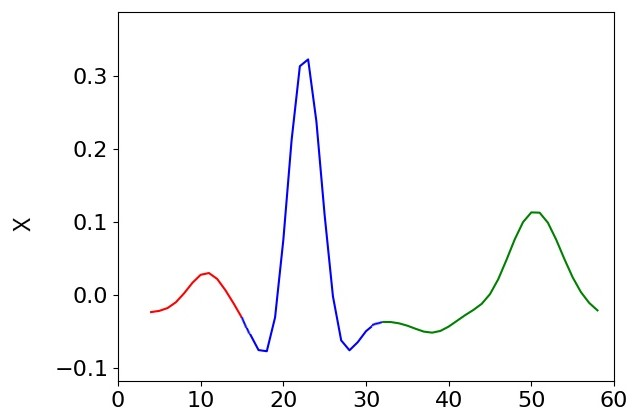
\includegraphics[width=1\textwidth]{immagini/lead_x.png}
            \captionsetup{justification=centering}
            \caption{}
            \label{fig:lead_x}
        \end{subfigure}
        \begin{subfigure}{\textwidth}
            \centering
            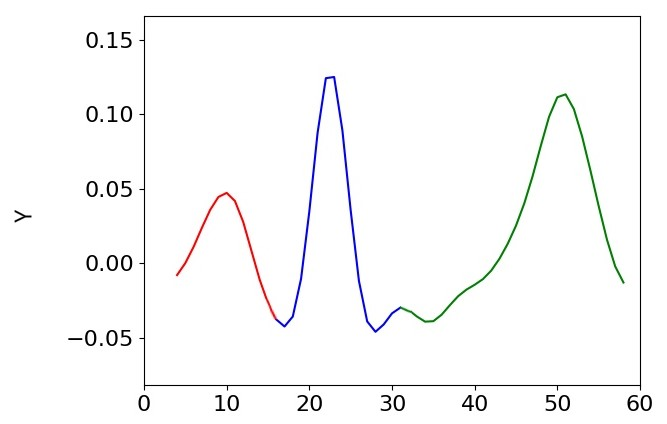
\includegraphics[width=1\textwidth]{immagini/lead_y.png}
            \captionsetup{justification=centering}
            \caption{}
            \label{fig:lead_y}
        \end{subfigure}
        \begin{subfigure}{\textwidth}
            \centering
            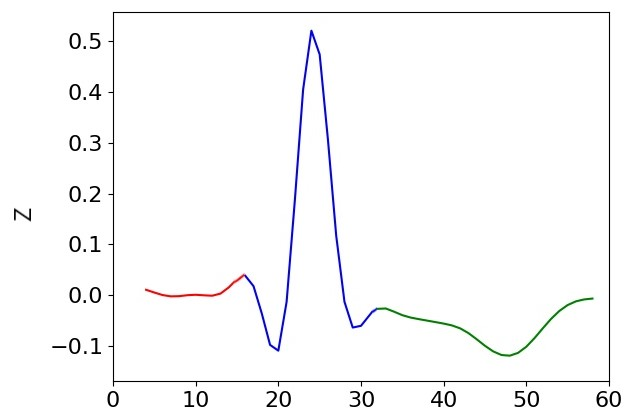
\includegraphics[width=1\textwidth]{immagini/lead_z.png}
            \caption{}
            \label{fig:lead_z}
        \end{subfigure}
    \end{subfigure}
    \begin{subfigure}{0.55\textwidth}
        \centering
        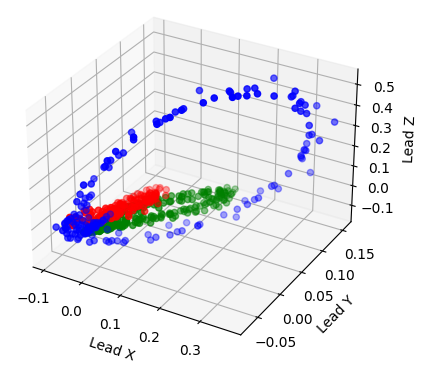
\includegraphics[width=1\linewidth]{immagini/frank3d.png}
        \captionsetup{justification=centering}
        \caption{}
        \label{fig:frank3d}
    \end{subfigure}
    \captionsetup{justification=centering}
    \caption{Le figure \ref{fig:lead_x}, \ref{fig:lead_y} e \ref{fig:lead_z} rappresentano rispettivamente i \textit{lead} X, Y e Z di un singolo battito di un ECG, mentre la figura \ref{fig:frank3d} rappresenta in modo tridimensionale un singolo ECG rispetto ai tre assi X, Y e Z.}
    \label{fig:ecg}
\end{figure}

\section{Deep Learning}
\label{sec:deep}

Il campo dell'analisi dell'ECG ha subito una trasformazione significativa grazie all'applicazione delle tecniche di \textit{deep learning}. Queste metodologie avanzate di intelligenza artificiale (IA) si sono dimostrate estremamente promettenti nel migliorare la precisione e l'efficienza nella diagnosi e nella classificazione delle condizioni cardiache. Nel corso degli anni, i ricercatori hanno sviluppato e raffinato una serie di architetture neurali, tra cui le reti neurali convoluzionali e le reti neurali ricorrenti per analizzare in modo automatico ed efficiente gli ECG.

In particolare le reti neurali convoluzionali, grazie alla loro capacità di apprendere automaticamente le caratteristiche rilevanti dai dati, si sono dimostrate specificatamente adatte per la classificazione delle aritmie cardiache. Sono infatti in grado di catturare pattern complessi ed identificare segnali di interesse, consentendo ai medici di ottenere risultati più accurati e tempestivi nella diagnosi di malattie cardiache. Le reti neurali ricorrenti, d'altra parte, sono in grado di modellare le dipendenze temporali presenti negli ECG e sono utilizzate per compiti come la rilevazione di anomalie e la predizione di eventi cardiaci.

Un aspetto chiave nell'applicazione del \textit{deep learning} all'analisi degli ECG è la disponibilità di dataset di addestramento ampi e di alta qualità. Questi dataset contengono migliaia di registrazioni ECG annotate da esperti, consentendo alle reti neurali di apprendere dai casi precedenti e di generare predizioni accurate su nuovi dati. Tuttavia, la raccolta e l'annotazione di questi dataset rappresentano ancora una sfida significativa che richiede un notevole sforzo umano e una collaborazione tra i medici ed i ricercatori.

L'applicazione del \textit{deep learning} all'analisi dell'ECG offre molte opportunità, ma presenta anche alcune sfide da affrontare. La robustezza della rete alle variazioni del segnale, la spiegabilità delle decisioni prese dalla rete stessa e la necessità di personalizzazione per adattarsi a diversi contesti clinici, sono solo alcune delle questioni da considerare. Inoltre, l'integrazione delle tecnologie di \textit{deep learning} nella pratica clinica richiede un'attenta valutazione dei rischi, della sicurezza e dell'etica.

Una delle principali sfide nell'applicazione del \textit{deep learning} agli ECG è la scarsità di dati etichettati a disposizione. L'etichettatura accurata dei dati richiede la competenza di medici esperti per identificare ed annotare le anomalie cardiache. Questo processo può essere oneroso e può richiedere molto tempo. Di conseguenza, spesso si dispone di un numero limitato di dati etichettati, il che può influire sulle capacità delle reti neurali di generalizzare ed ottenere risultati accurati. Poiché gli ECG possono variare notevolmente tra i pazienti, anche in presenza della stessa condizione cardiaca, la variabilità può essere dovuta a numerosi fattori come l'età, il sesso, la posizione degli elettrodi e le condizioni fisiologiche individuali. Questa variabilità rappresenta una sfida per le reti neurali in quanto devono essere in grado di riconoscere ed adattarsi a queste differenze individuali al fine di ottenere risultati accurati ed affidabili.

Tuttavia, prima di poter applicare algoritmi di analisi e modelli di IA, è necessario effettuare un adeguato \textit{pre-processing} degli ECG. Il \textit{pre-processing} svolge un ruolo cruciale nel miglioramento della qualità dei segnali, eliminando il rumore indesiderato e preparando i dati per una corretta analisi. Gli ECG sono spesso affetti da rumore, come interferenze elettriche o movimenti muscolari, che possono compromettere la precisione delle analisi successive. Il \textit{pre-processing} degli ECG prevede l'applicazione di tecniche di filtraggio per rimuovere il rumore indesiderato ed isolare il segnale cardiaco puro. Ciò consente di ottenere una rappresentazione più pulita del segnale e facilita l'identificazione di pattern ed anomalie significative. Ad esempio, \textit{l'artefatto di linea di base} è un fenomeno comune negli ECG, causato da movimenti del paziente o dalla posizione degli elettrodi, e dunque questo tipo di rumore può interferire con la corretta interpretazione dei segnali da parte delle reti neurali. Attraverso queste tecniche di \textit{pre-processing} è quindi possibile ridurre l'artefatto di linea di base ed ottenere un segnale più stabile ed accurato~\cite{use}.

Nonostante queste sfide, i risultati ottenuti finora sono estremamente promettenti: la combinazione di competenze mediche e conoscenze di \textit{deep learning} sta aprendo nuove prospettive nell'analisi degli ECG, consentendo diagnosi più accurate, tempestive e personalizzate per i pazienti. L'utilizzo del \textit{deep learning} nell'analisi degli ECG rappresenta un campo di ricerca in rapida evoluzione e sicuramente continuerà a fornire contributi significativi alla pratica clinica cardiologica.

Per concludere, il potenziale del \textit{deep learning} nell'analisi degli ECG è enorme: l'insieme dei modelli avanzati di IA e dell'esperienza clinica dei medici offre un'opportunità senza precedenti per migliorare la diagnosi, la prognosi e la gestione delle malattie cardiache. La ricerca continua e la collaborazione tra medici e ricercatori saranno fondamentali per sfruttare totalmente il potenziale di queste tecnologie e portare benefici tangibili ai pazienti affetti da patologie cardiache.

\section{Obiettivo della ricerca}
\label{sec:obiettivo}

L'obiettivo della ricerca è stato quello di ricostruire, a partire da un elettrocardiogramma (ECG), il segnale che idealmente lo precederebbe e susseguirebbe nel tempo. Ciò ha richiesto l'analisi preliminare degli ECG presi in esame, in modo tale da poter successivamente definire ed addestrare la \textit{convolutional neural network} (CNN) tramite l'utilizzo del \textit{deep learning} per far sì che si riuscisse a prevedere l'evoluzione dell'ECG stesso.

Poiché le cliniche utilizzano ancora moltissimo gli ECG cartacei che hanno una durata di dieci secondi, dei quali i primi cinque mostrano i primi 6 \textit{lead} dell'ECG mentre i restanti cinque mostrano i restanti 6 \textit{lead} dell'ECG, l'obiettivo è stato quello di ricostruire i \textit{lead} che non vengono osservati, e cioè i primi 6 nei secondi cinque secondi, ed i secondi 6 nei primi cinque secondi, partendo dall'informazione iniziale in possesso.

Per condurre l'intero processo si è ricorso all'utilizzo del linguaggio \textit{Python}.

\chapter{Materiali e metodi utilizzati}
\label{chap:materiali}

\section{Dataset}
\label{sec:dataset}

Il dataset da utilizzare per effettuare la ricerca è stato individuato in \textit{PTB-XL}, un dataset esteso di ECG sviluppato in Germania e contenente registrazioni di segnali ad alta risoluzione provenienti da pazienti con una vasta varietà di condizioni cardiache. Questo dataset è stato creato per scopi di ricerca e fornisce un'ampia gamma di segnali, tra cui dati a 12 derivazioni ed a 15 derivazioni. Il dataset contiene sia ECG di pazienti sani che ECG di pazienti affetti da anomalie cardiache, consentendo agli utenti di esplorare ed analizzare diversi casi clinici. Per questi motivi è diventato una risorsa preziosa per gli esperti di \textit{deep learning} ed IA nel campo della cardiologia, poiché fornisce un ampio set di dati per addestrare e valutare le reti neurali per la diagnosi e la classificazione delle patologie cardiache~\cite{datasetdistro}.

\textit{PTB-XL} è un ampio dataset di 21799 ECG a 12 derivazioni provenienti da 18869 pazienti, con una durata di 10 secondi ciascuno. I dati delle forme d'onda grezze sono stati annotati da uno o due cardiologi che hanno assegnato potenzialmente più dichiarazioni ECG a ciascun record. Tutte le 71 diverse dichiarazioni ECG sono conformi allo standard \textit{SCP-ECG} ed includono dichiarazioni diagnostiche, di forma e di ritmo. Inoltre, il dataset è integrato da metadati dettagliati sulla demografia, sulle caratteristiche di infarto, sulla probabilità delle dichiarazioni diagnostiche e sulle proprietà segnalate. I dati delle forme d'onda sono stati raccolti nel corso di quasi sette anni, tra l'ottobre 1989 ed il giugno 1996. Durante il processo di pubblicazione nel 2019, il dataset preesistente è stato ottimizzato con particolare attenzione all'usabilità ed all'accessibilità per la comunità di \textit{deep learning}, difatti le forme d'onda ed i metadati sono stati convertiti in formati di dati che possono essere facilmente elaborati da software standard~\cite{dataset}~\cite{datasetref}.

Inoltre, il dataset contiene due versioni per ogni ECG, una con frequenza di campionamento pari a \texttt{100 Hz}, ed una con frequenza di campionamento pari a \texttt{500 Hz}. Per questa ricerca, sono stati selezionati gli ECG con frequenza di campionamento pari a \texttt{100 Hz}.

\section{Selezione dei segnali e loro filtraggio}
\label{sec:filtraggio}

Poiché il dataset considerato include anche ECG di pazienti affetti da anomalie cardiache, è stato dapprima necessario effettuare un filtraggio dei segnali in maniera tale da considerare esclusivamente gli ECG di pazienti sani.

Dalla tabella \ref{tab:dataset} riportata di seguito si può evincere il numero di ECG utilizzati durante la ricerca:

\begin{table}[H]
    \centering
    \begin{tabular}{|>{\centering\arraybackslash}m{3.5cm}|c|c|}
	\hline Numero di record & Superclasse & Breve descrizione \\ \hline
	9514 & NORM & ECG normali \\
	5469 & MI & Infarto del miocardio \\
	5235 & STTC & Anomalia dell'onda ST/T \\
    4898 & CD & Disturbo di conduzione \\
    2649 & HYP & Ipertrofia \\ \hline
    \end{tabular}
    \captionsetup{justification=centering}
    \caption{Distribuzione delle dichiarazioni diagnostiche aggregate in superclassi. Nota: La somma delle dichiarazioni supera il numero dei record presenti nel dataset a causa della possibile presenza di più etichette per record.}
    \label{tab:dataset}
\end{table}

Il filtraggio è stato eseguito per mezzo di due frequenze minima e massima rispettivamente pari a \texttt{0.5 Hz} e \texttt{15 Hz} ed utilizzate per calcolare le due frequenze di taglio bassa ed alta. A loro volta queste sono state impiegate nel \textit{filtro Butterworth} implementato, con lo scopo di mantenere il più piatto possibile il modulo della risposta in frequenza nella banda passante, per poi applicare successivamente ad ogni ECG il cosiddetto \textit{filtraggio di Gustafson}, che ha permesso di migliorare la qualità degli ECG, riducendo il rumore ed altre interferenze indesiderate, specialmente ai bordi del segnale. La tecnica utilizzata è nota come \texttt{filtfilt} o \textit{filtraggio a fase zero}, nel quale un segnale viene elaborato in modo da attenuare le componenti indesiderate mentre viene mantenuto invariato il ritardo temporale tra le diverse frequenze del segnale stesso. In altre parole, il \textit{filtraggio a fase zero} è una tecnica che rimuove il ritardo nel segnale filtrato, consentendo di ottenere una rappresentazione più accurata del segnale originale. Questo è particolarmente importante nei casi in cui la conservazione del ritardo tra le diverse frequenze del segnale è cruciale per l'analisi, come in questo contesto di ricerca.

Dalla figura \ref{fig:filtraggio} riportata di seguito si possono notare le differenze tra il segnale originale ed il segnale filtrato:

\begin{figure}[H]
    \centering
    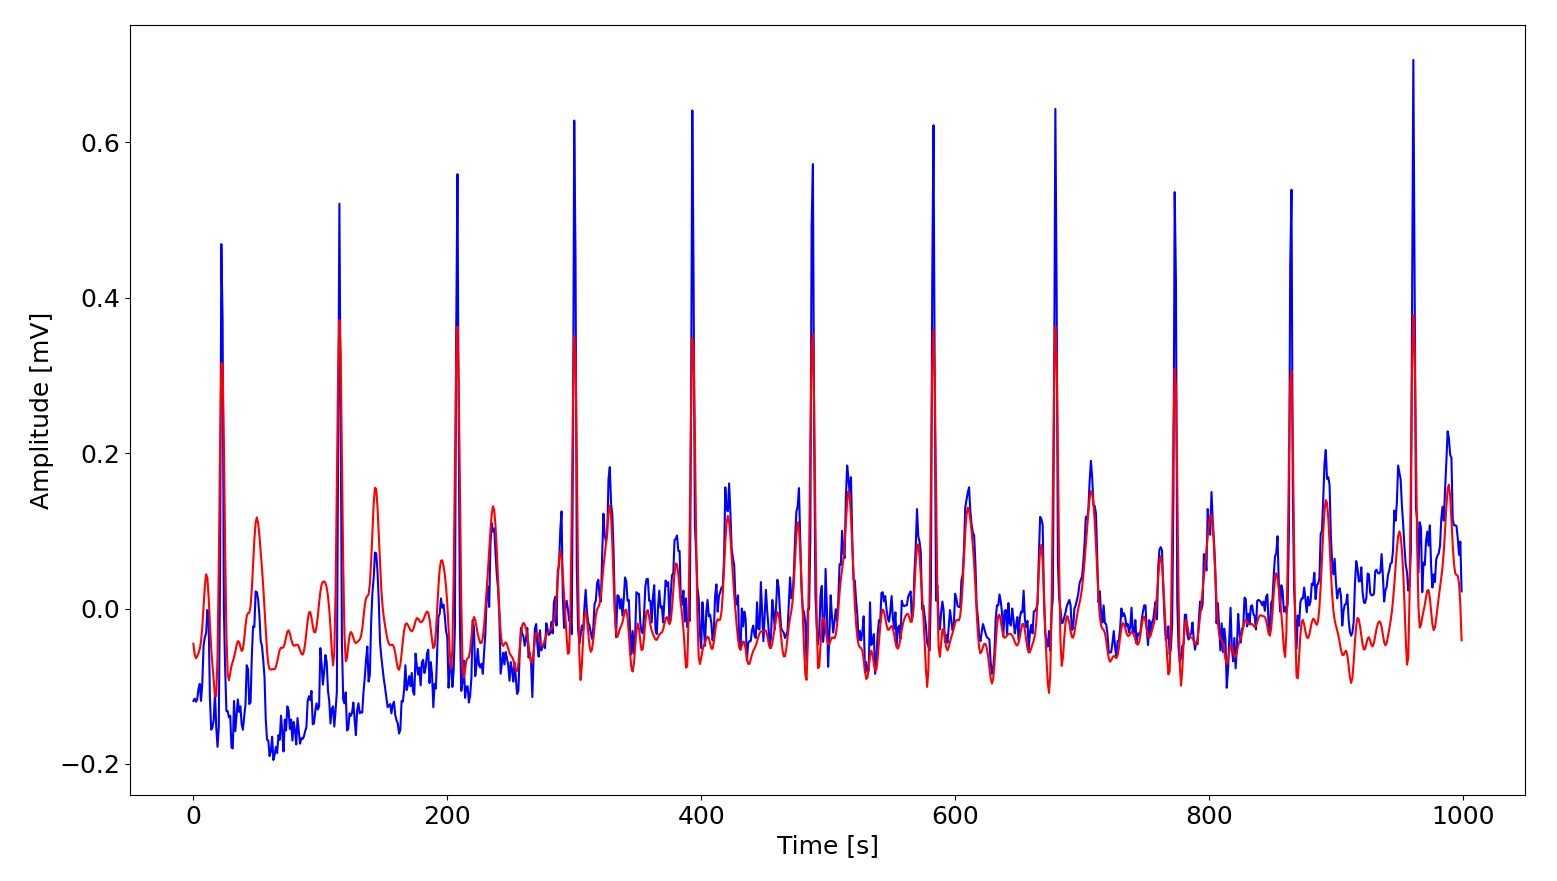
\includegraphics[width=1\textwidth]{immagini/filtraggio.png}
    \captionsetup{justification=centering}
    \caption{Differenze tra il segnale originale (in blu) ed il segnale filtrato (in rosso) in seguito all'applicazione del filtraggio di Gustafson.}
    \label{fig:filtraggio}
\end{figure}

Infine lo snippet \ref{snippet:filtraggio} riportato di seguito illustra il codice della funzione utilizzata per effettuare le operazioni sopra citate:

\lstset{language=Python}
\begin{lstlisting}[aboveskip=15pt, belowskip=15pt, basicstyle=\fontsize{8}{10}\selectfont, keywordstyle=\color{blue}, breaklines=true, label=snippet:filtraggio]
def FilterSignals(signal, fs = 100, do_plot = False):
    f_low = 0.5
    f_high = 15
    order = 3
    nyquist_freq = 0.5 * fs
    lowcut = f_low / nyquist_freq
    highcut = f_high / nyquist_freq
    b, a = butter(order, [lowcut, highcut], btype = 'band')
    filtered_signal = filtfilt(b, a, signal, axis = 1, method = 'gust')
    if do_plot:
        plt.figure(figsize = (10, 4))
        plt.plot(signal, 'b-', label = 'Original ecg')
        plt.plot(filtered_signal, 'r-', label = 'Filtered ecg')
        plt.xlabel('Time [s]')
        plt.ylabel('Amplitude [mV]')
        plt.legend()
        plt.grid(True)
        plt.show()
    return filtered_signal
\end{lstlisting}

\section{Matrice inversa di Dower}
\label{sec:matrice}

La trasformazione inversa di Dower si riferisce a un processo utilizzato nell'analisi degli ECG per ottenere una rappresentazione spaziale dei segnali cardiaci. Durante la trasformazione di Dower, gli ECG vengono proiettati su un insieme di assi ortogonali definiti come \textit{lead} di Frank, che rappresentano le direzioni del flusso elettrico che passano attraverso il cuore. La trasformazione inversa di Dower è quindi il processo che consente di ottenere nuovamente i segnali dalla loro rappresentazione spaziale secondo i \textit{lead} di Frank.

Attraverso questa trasformazione inversa, è possibile ottenere una rappresentazione dei segnali nel dominio temporale e di ampiezza, tornando alla visualizzazione dei segnali come tracciati temporali delle variazioni di tensione nel tempo~\cite{dower}.

La tabella \ref{tab:dower} riportata di seguito indica i pesi ottenuti a partire dalla matrice inversa di Dower~\cite{dowerecg}:

\begin{table}[H]
	\centering
    \begin{tabular}{|*{4}{>{\centering\arraybackslash}m{2.5cm}|}}
    \hline \textit{Lead} & X & Y & Z \\
    \hline
	V1 & -0.17245 & 0.057224 & -0.22891 \\
	V2 & -0.07377 & -0.018954 & -0.31001 \\
	V3 & 0.12222 & -0.10637 & -0.24588 \\
	V4 & 0.23103 & -0.021986 & -0.063351 \\
    V5 & 0.23931 & 0.040947 & 0.054782 \\
    V6 & 0.19358 & 0.048257 & 0.10849 \\
    I & 0.15608 & -0.22739 & 0.021654 \\ 
    II & -0.0099152 & 0.88653 & 0.10207 \\ \hline
    \end{tabular}
    \captionsetup{justification=centering}
    \caption{Pesi ottenuti a partire dalla matrice inversa di Dower, in questo caso trasposta rispetto alla matrice originale.}
    \label{tab:dower}
\end{table}

Dalla figura \ref{fig:frank2d} riportata di seguito invece, si può notare la rappresentazione bidimensionale dei tre \textit{lead} X, Y e Z di un singolo ECG:

\begin{figure}[H]
    \centering
    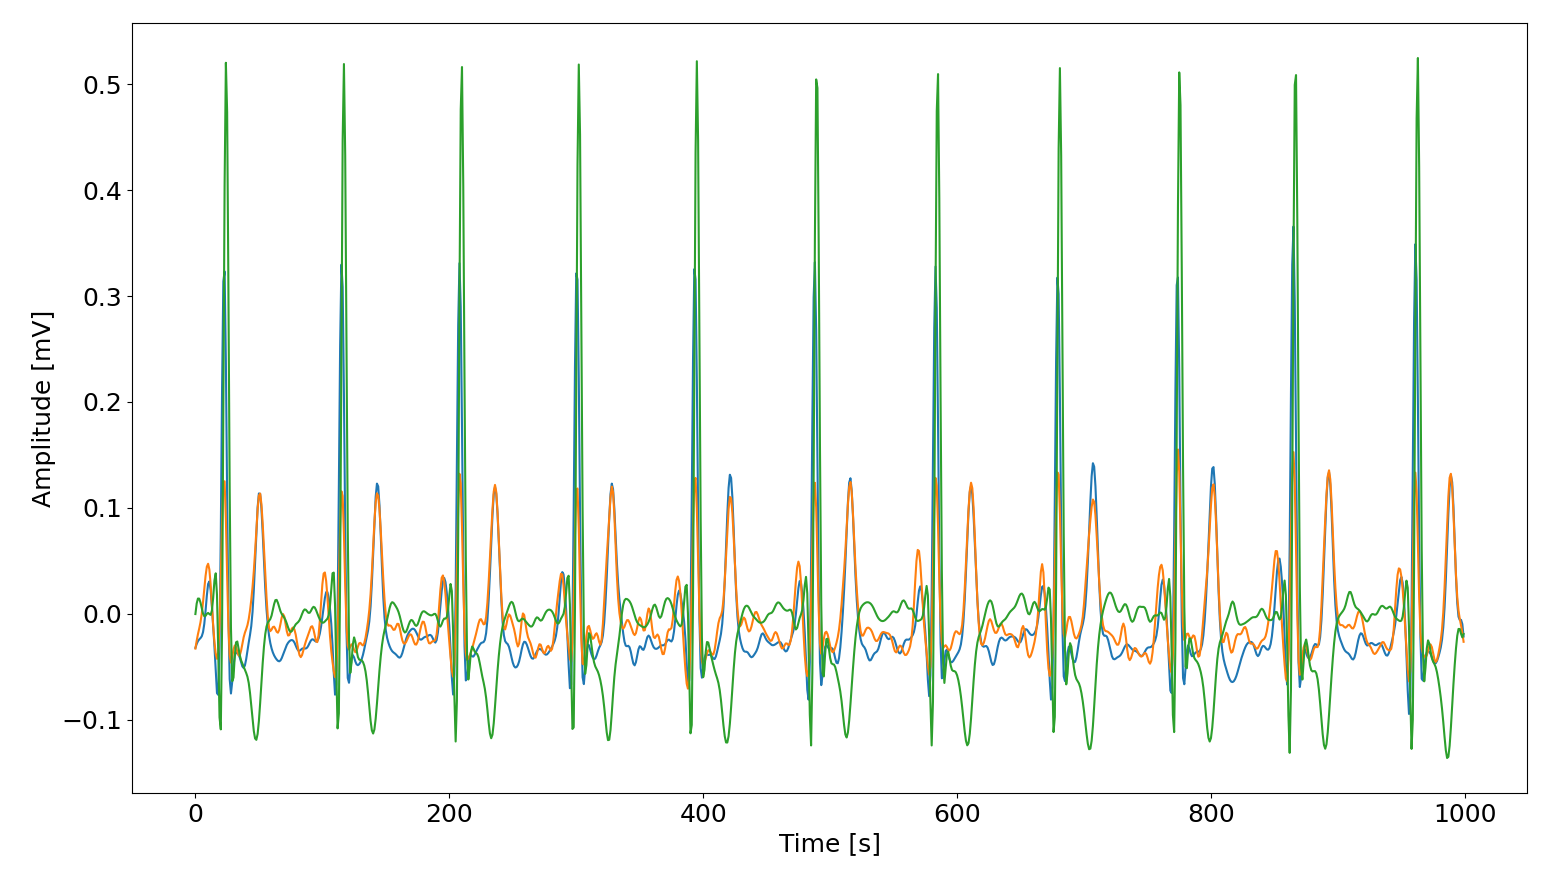
\includegraphics[width=1\textwidth]{immagini/frank2d.png}
    \captionsetup{justification=centering}
    \caption{Rappresentazione bidimensionale dei tre \textit{lead} X, Y e Z di un singolo ECG.}
    \label{fig:frank2d}
\end{figure}

Infine lo snippet \ref{snippet:dower} riportato di seguito illustra il codice della funzione utilizzata per l'applicazione della trasformazione inversa di Dower:

\lstset{language=Python}
\begin{lstlisting}[aboveskip=15pt, belowskip=15pt, basicstyle=\fontsize{8}{10}\selectfont, keywordstyle=\color{blue}, breaklines=true, label=snippet:dower]
def ApplyInverseMatrix(signal, do_plot = False):
    matrix = pd.read_csv('inverse_dower.csv', header = None)
    weights = torch.tensor(matrix.values, dtype = torch.float64)
    ponderate_ecg = torch.matmul(weights, signal)
    if do_plot:
        plt.figure(figsize = (10, 6))
        plt.plot(ponderate_ecg.T)
        plt.xlabel('Time [s]')
        plt.ylabel('Amplitude [mV]')
        plt.title('ECG Leads: X, Y, Z')
        plt.show()
    return ponderate_ecg
\end{lstlisting}

\section{Entropia}
\label{sec:entropia}

Per entropia di una matrice si intende una misura della sua complessità o della sua incertezza. In generale, l’entropia di una distribuzione uniforme ha entropia massima possibile, mentre l'entropia di una costante ha sempre entropia uguale a zero. Dunque maggiore è l’entropia, maggiore è la diversità tra i dati.

L'obiettivo è stato quello di ricostruire i sei segnali [$ V_{1}, V_{2}, V_{3}, V_{4}, V_{5}, V_{6} $] a partire dagli altri sei segnali [$ I, II, III, aV_{R}, aV_{L}, aV_{F} $]. I primi stanno principalmente sul piano orizzontale mentre i secondi sul piano frontale. Questo significa che in realtà non sarebbe possibile determinare ognuno dei primi segnali [$ V_{1}, V_{2}, V_{3}, V_{4}, V_{5}, V_{6} $] a partire dai secondi segnali [$ I, II, III, aV_{R}, aV_{L}, aV_{F} $], poiché non vale la formula (\ref{eq:lead}):

\begin{equation}
    V_{n} = f_{n}(I, II, III, aV_{R}, aV_{L}, aV_{F})
    \label{eq:lead}
\end{equation}

Tuttavia ciò in realtà dipende da quanto è probabile $ V_{n} $ dati i valori degli altri \textit{lead}. Ad esempio se $ V_{n} $ fosse sempre pari ad \texttt{1 mV} sarebbe possibile scrivere la funzione $ f_{n} $, ed in tal caso sarebbe pari a $ f_{n} = 1 $. Per avere però $ f = 0 $ bisognerebbe avere che il \textit{lead} $ V_{1} $ punti sempre ad \texttt{1 mV} sul piano orizzontale ottenendo dunque un impulso come istogramma, ed ottenendo un valore di entropia minima.

Detto ciò, è possibile proiettare le derivazioni di Frank X, Y e Z sul piano bidimensionale in modo tale da calcolarne l'istogramma; ed usandolo come stima della densità di probabilità è possibile calcolarne l'entropia per comprendere quanto sia predicibile.

Il passo immediatamente successivo è stato calcolare le distribuzioni bidimensionali relative ad ogni istogramma, relativo, a sua volta, ad ogni ECG.

Grazie ad ognuna di queste distribuzioni, è stato dunque possibile calcolarne totalmente la somma per rappresentarne un'unica ripartizione totale nel tempo. Tale ripartizione, rappresentata sugli assi tridimensionali X, Y e Z, individua le celle delle distribuzioni nelle quali si trovano i punti di cui ogni ECG è costituito, ed è di fondamentale importanza per il calcolo dell'entropia.

Dalla figura \ref{fig:hist} riportata di seguito si può evincere la rappresentazione bidimensionale dell'istogramma di un singolo battito di un certo ECG:

\begin{figure}[H]
    \centering
    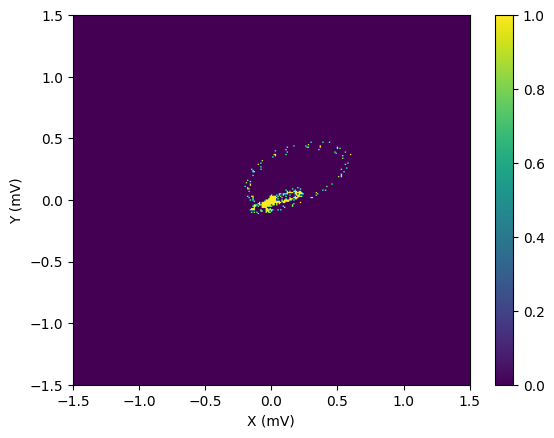
\includegraphics[width=0.65\textwidth]{immagini/hist.png}
    \captionsetup{justification=centering}
    \caption{Rappresentazione bidimensionale dell'istogramma della distribuzione bidimensionale di un singolo battito di un ECG.}
    \label{fig:hist}
\end{figure}

La figura \ref{fig:hists} riportata di seguito invece, illustra la rappresentazione della matrice contenente la somma delle distribuzioni bidimensionali relative ad ogni battito di tutti gli ECG di tutti i pazienti considerati:

\begin{figure}[H]
    \centering
    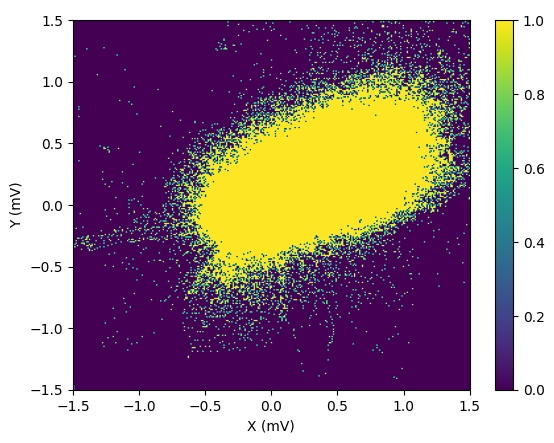
\includegraphics[width=0.65\textwidth]{immagini/hists.png}
    \captionsetup{justification=centering}
    \caption{Rappresentazione della matrice contenente la somma delle distribuzioni bidimensionali relative ad ogni battito di tutti gli ECG.}
    \label{fig:hists}
\end{figure}

L’entropia può essere calcolata utilizzando diverse formule, a seconda del contesto specifico. Ad esempio, per una matrice di probabilità, l’entropia può essere calcolata utilizzando una generalizzazione della formula (\ref{eq:shannon}) dell’entropia di Shannon, riportata di seguito:

\begin{equation}
    H = - \sum_{x,y} p(x,y) \log_2(p(x,y))
    \label{eq:shannon}
\end{equation}

La formula rappresenta l'entropia di Shannon congiunta $ H $ di due variabili discrete $ x $ ed $ y $, ovvero una generalizzazione a due o più variabili della formula di Shannon. In particolare, il simbolo $ \sum_{x,y} $ indica una sommatoria su tutte le possibili combinazioni di valori di $ x $ ed $ y $, $ p(x,y) $ rappresenta la probabilità congiunta che le variabili $ x $ ed $ y $ assumano determinati valori contemporaneamente, mentre $ \log_2(p(x,y)) $ è il logaritmo binario della probabilità congiunta di $ x $ ed $ y $, ovvero la probabilità che entrambe le variabili assumano determinati valori contemporaneamente.

Lo snippet \ref{snippet:entropia} riportato di seguito mostra il codice della funzione utilizzata per il calcolo dell'entropia, sulla base della formula illustrata sopra:

\lstset{language=Python}
\begin{lstlisting}[aboveskip=15pt, belowskip=15pt, basicstyle=\fontsize{8}{10}\selectfont, keywordstyle=\color{blue}, breaklines=true, label=snippet:entropia]
def CalculateEntropy(hists_matrix):
    probabilities = hists_matrix / np.sum(hists_matrix)
    entropy = -np.sum(probabilities * np.log2(probabilities + np.finfo(float).eps))
    max_entropy = np.log2(hists_matrix.shape[0] * hists_matrix.shape[1])
    print(entropy / max_entropy)
\end{lstlisting}

Infine, è stata utilizzata un'ulteriore formula (\ref{eq:entropia}) durante la ricerca, riportata di seguito, che restituisce un indice numerico chiamato \textit{indice di predicibilità} compreso tra \texttt{0} ed \texttt{1}, per cui \texttt{0} significa che si tratta di una distribuzione uniforme poiché $ H = H_{u} $, dove $ H_{u} $ è l'entropia di una distribuzione uniforme, e dunque è \textit{completamente non predicibile}, mentre \texttt{1} significa che non si tratta di una distribuzione uniforme poiché $ H = 0 $ e dunque è \textit{completamente predicibile} e cioè \textit{costante}:

\begin{equation}
    h = \frac{H_{u} - H}{H_{u}}
    \label{eq:entropia}
\end{equation}

\section{Modellazione del problema}
\label{sec:modellazione}

Il modello che è stato costruito è basato su una CNN, per via dei risultati estramemente promettenti ottenuti dal loro utilizzo in altri studi, e poiché sono molto efficienti in termini di risorse computazionali, rendendole adatte per l'addestramento su grandi set di dati, come nel caso di questa ricerca~\cite{ribeiro}~\cite{hannun}.

Il modello, indipendentemente dalla complessità delle varie CNN implementate, riceve come dati in input 12 \textit{lead} divisi in due blocchi da 6, ognuno dei quali della durata di cinque secondi. L'informazione iniziale in possesso è dunque doppia, e cioè i primi 6 \textit{lead} nei primi cinque secondi, ed i secondi 6 \textit{lead} nei secondi cinque secondi. L'output del modello stesso, invece, sono i \textit{lead} che non vengono osservati, e cioè i primi 6 nei secondi cinque secondi, ed i secondi 6 nei primi cinque secondi.

Il modello che è stato costruito si può riassumere matematicamente con l'equazione (\ref{eq:modello}) riportata di seguito, dove $ x $ indica gli ECG che costituiscono l'input, mentre $ y $ indica gli ECG che costituiscono l'output:

\begin{equation}
    y = f(x)
    \label{eq:modello}
\end{equation}

Tuttavia, il problema in questione non è banale poiché ogni ECG è un segnale complesso e multi-dimensionale, inoltre è composto da diverse componenti, tra cui l'onda P, l'onda Q, l'onda R, l'onda S e l'onda T, ed ogni componente ha una propria forma ed una propria durata, e la loro relazione reciproca è importante per l'interpretazione di ognuno degli ECG.

\section{Rete neurale convoluzionale}
\label{sec:network}

\subsection{Descrizione formale}
\label{subsec:descrizione}

Durante la ricerca sono state implementate e testate numerose CNN, tutte molto diverse tra loro, in modo tale da poter ottenere molti e differenti risultati riguardo la ricostruzione degli ECG.

Ogni CNN è stata implementata come una classe, ognuna delle quali definita da due funzioni \texttt{init()} e \texttt{forward()}, rispettivamente utilizzate per creare un'istanza della classe che rappresenta la CNN e per definire il flusso di dati attraverso la rete, dove i dati in input vengono propagati attraverso i vari strati per generare l'output finale.

Durante la fase di inizializzazione, vengono definiti i vari strati della CNN, come i layer convoluzionali, i layer di \textit{pooling}, i layer completamente connessi e le funzioni di attivazione. All'interno della funzione \texttt{init()}, vengono impostati anche i parametri fondamentali della rete, come ad esempio le dimensioni dei filtri convoluzionali, il numero di \textit{feature maps}, le dimensioni delle funzioni di \textit{pooling}, le dimensioni di input ed output, e molti altri parametri che ne influenzano le prestazioni. Inoltre, in questa fase possono essere create altre variabili necessarie per la gestione dei dati e dei pesi dei layer.

All'interno della funzione \texttt{forward()} invece, vengono eseguite le operazioni di convoluzione, di \textit{pooling} e di attivazione, consentendo alla rete di apprendere rappresentazioni complesse dai dati in input. Durante l'esecuzione della funzione \texttt{forward()}, i dati in input passano attraverso i vari strati, ed i pesi vengono applicati alle \textit{feature maps} per produrre l'output finale. Ogni strato dispone dei propri pesi e dei propri \textit{bias} che vengono aggiornati durante la fase di addestramento della rete, in modo che la CNN possa apprendere come riconoscere pattern e caratteristiche rilevanti presenti nei dati. È importante sottolineare che la funzione \texttt{forward()} viene eseguita successivamente, e cioè durante la fase di valutazione della rete, quando questa viene utilizzata per fare previsioni sui nuovi dati in input. Questo processo di propagazione successivo consente alla CNN di produrre l'output desiderato in base ai pesi acquisiti durante la fase di addestramento.

\subsection{Prima CNN}
\label{subsec:prima}

Lo snippet \ref{snippet:prima} riportato di seguito rappresenta il codice di una delle prime CNN implementate e testate, la quale, però, non ha restituito i risultati sperati inizialmente:

\lstset{language=Python}
\begin{lstlisting}[aboveskip=15pt, belowskip=15pt, basicstyle=\fontsize{8}{10}\selectfont, keywordstyle=\color{blue}, breaklines=true, label=snippet:prima]
class ConvNet(nn.Module):
    def __init__(self, input_shape):
        super(ConvNet, self).__init__()
        self.input_shape = input_shape
        self.conv1 = nn.Conv1d(in_channels = self.input_shape[0], out_channels = 32, kernel_size = 8)
        self.conv2 = nn.Conv1d(in_channels = 32, out_channels = 64, kernel_size = 8)
        self.maxpool = nn.MaxPool1d(kernel_size = 2)
        self.flatten = nn.Flatten()
        self.fc1 = nn.Linear(7616, 128)
        self.relu = nn.ReLU()
        self.output = nn.Linear(128, self.input_shape[0] * self.input_shape[1])
    def forward(self, x):
        with open(f'{OUTPUTS_DIRECTORY}/model_settings.txt', 'w') as file:
            file.write(f'conv_kernel_size = {self.conv1.kernel_size[0]}, maxpool_kernel_size = {self.maxpool.kernel_size}')
        x = x.to(device)
        x = x.type(torch.DoubleTensor)
        x = x.to(device)
        x = self.conv1(x)
        x = self.relu(x)
        x = self.maxpool(x)
        x = self.conv2(x)
        x = self.relu(x)
        x = self.maxpool(x)
        x = self.relu(x)
        x = self.flatten(x)
        x = self.fc1(x)
        x = self.relu(x)
        x = self.output(x)
        x = torch.reshape(x, (-1, self.input_shape[0], self.input_shape[1]))
        return x
\end{lstlisting}

La figura \ref{fig:prima} riportata di seguito rappresenta, sotto forma di diagramma di flusso, i layer che costituiscono il codice \ref{snippet:prima} della prima CNN, riportato immediatamente sopra:

\begin{figure}[H]
    \centering
    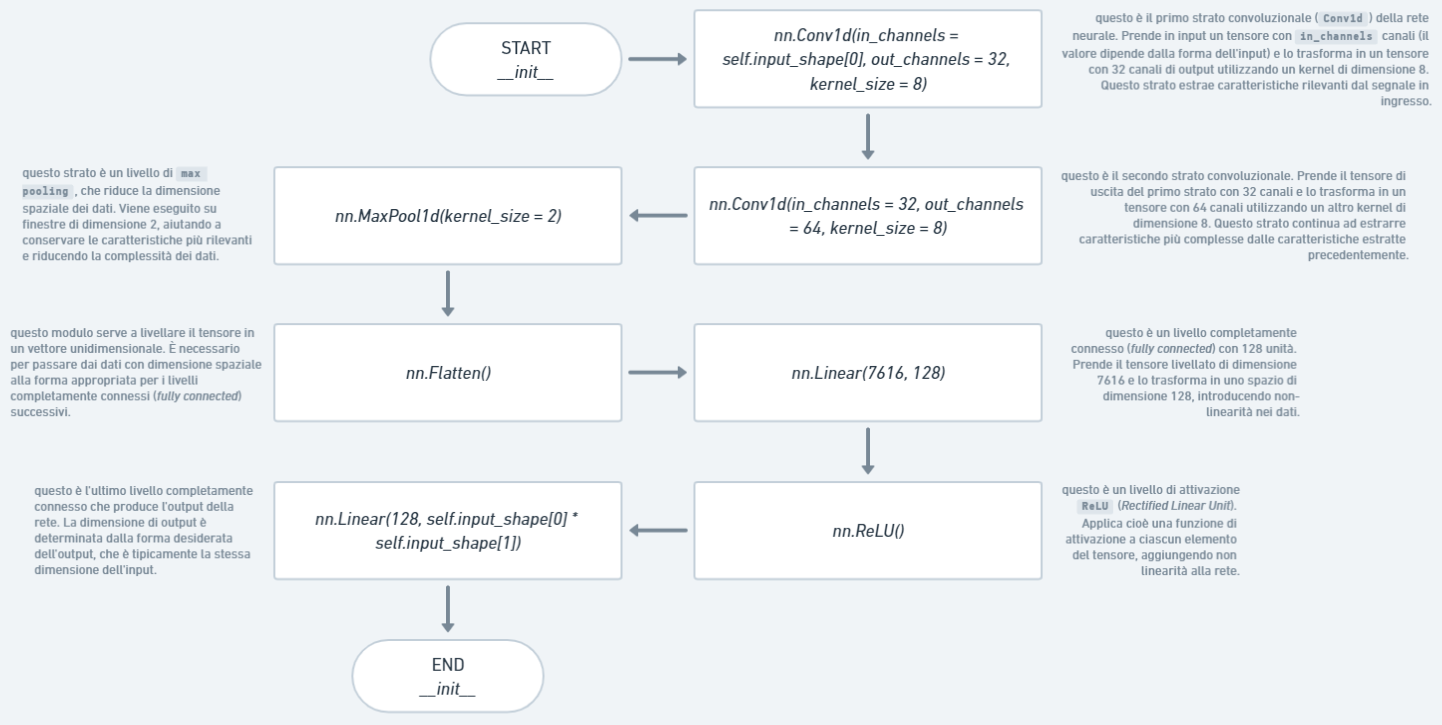
\includegraphics[width=1\textwidth]{immagini/prima.png}
    \captionsetup{justification=centering}
    \caption{Rappresentazione del codice della prima CNN come diagramma di flusso.}
    \label{fig:prima}
\end{figure}

Questa prima CNN include solamente una \textit{ConvNet} il cui codice è formato da un insieme di layer convoluzionali che si ripetono diverse volte nella funzione \texttt{forward()} agendo sui parametri in input.

\subsection{Seconda CNN}
\label{subsec:seconda}

Lo snippet \ref{snippet:seconda} riportato di seguito rappresenta invece il codice di un'altra CNN definibile come ``intermedia'' in quanto a difficoltà considerando tutte le CNN utilizzate durante la ricerca, anche se, tuttavia, anch'essa non ha restituito i risultati sperati:

\lstset{language=Python}
\begin{lstlisting}[aboveskip=15pt, belowskip=15pt, basicstyle=\fontsize{8}{10}\selectfont, keywordstyle=\color{blue}, breaklines=true, label=snippet:seconda]
class ResidualBlock(nn.Module):
    def __init__(self, in_channels, out_channels, kernel_size):
        super(ResidualBlock, self).__init__()
        self.conv = nn.Conv1d(in_channels, out_channels, kernel_size, padding = 'same')
        self.relu = nn.ReLU()
    def forward(self, x):
        x = x.to(device)
        x = x.type(torch.DoubleTensor)
        out = self.conv(x)
        out = self.relu(out)
        return x + out
class ConvNet(nn.Module):
    def __init__(self, input_shape):
        super(ConvNet, self).__init__()
        self.input_shape = input_shape
        self.conv1 = ResidualBlock(in_channels = self.input_shape[0], out_channels = self.input_shape[0], kernel_size = 32)
        self.conv2 = nn.Conv1d(in_channels = self.input_shape[0], out_channels = 32, kernel_size = 16)
        self.conv3 = ResidualBlock(in_channels = 32, out_channels = 32, kernel_size = 16)
        self.conv4 = nn.Conv1d(in_channels = 32, out_channels = 16, kernel_size = 5)
        self.conv5 = ResidualBlock(in_channels = 16, out_channels = 16, kernel_size = 5)
        self.conv6 = nn.Conv1d(in_channels = 16, out_channels = 128, kernel_size = 3)
        self.maxpool = nn.MaxPool1d(kernel_size = 2)
        self.flatten = nn.Flatten()
        self.fc1 = nn.Linear(6656, 128)
        self.relu = nn.ReLU()
        self.output = nn.Linear(128, self.input_shape[0] * self.input_shape[1])
    def forward(self, x):
        x = self.conv1(x)
        x = self.relu(x)
        x = self.maxpool(x)
        x = self.conv2(x)
        x = self.relu(x)
        x = self.maxpool(x)
        x = self.conv3(x)
        x = self.relu(x)
        x = self.maxpool(x)
        x = self.conv4(x)
        x = self.relu(x)
        x = self.conv5(x)
        x = self.relu(x)
        x = self.conv6(x)
        x = self.flatten(x)
        x = self.fc1(x)
        x = self.relu(x)
        x = self.output(x)
        x = torch.reshape(x, (-1, self.input_shape[0], self.input_shape[1]))
        return x
\end{lstlisting}

La figura \ref{fig:seconda} riportata di seguito rappresenta, sotto forma di diagramma di flusso, i layer che costituiscono il codice \ref{snippet:seconda} della seconda CNN, riportato immediatamente sopra:

\begin{figure}[H]
    \centering
    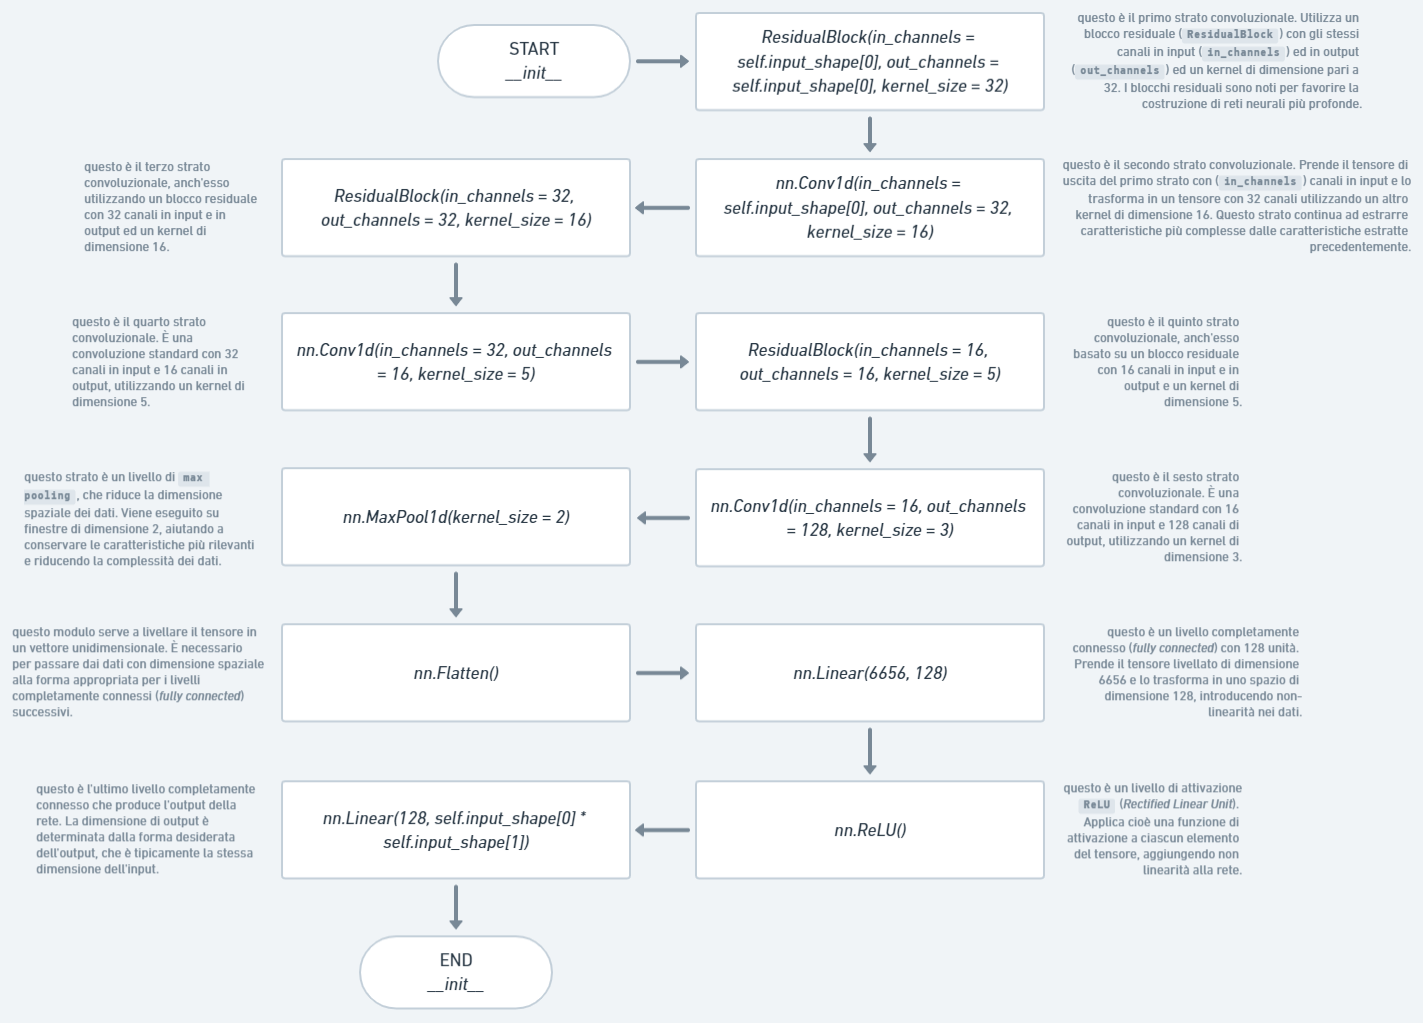
\includegraphics[width=1\textwidth]{immagini/seconda.png}
    \captionsetup{justification=centering}
    \caption{Rappresentazione del codice della seconda CNN come diagramma di flusso.}
    \label{fig:seconda}
\end{figure}

Questa CNN ``intermedia'', include solamente una \textit{ConvNet} il cui codice è formato da un insieme di layer convoluzionali uniti ad una componente esterna chiamata \textit{Residual Block}, introdotta per affrontare il problema del degrado delle performance quando le reti diventano più profonde, ed implementata come una classe che rappresenta un modulo autonomo della CNN, progettato per apprendere le caratteristiche più raffinate dai dati. L'idea di fondo è quella di consentire al flusso di dati di bypassare uno o più strati di convoluzione, in modo tale che, ogni flusso bypassato, venga poi aggiunto alle uscite dei successivi layer convoluzionali. In questo modo l'aggiunta del flusso bypassato migliora la propagazione dei gradienti a ritroso durante l'addestramento, facilitando l'apprendimento di rappresentazioni più efficaci. Implementando il \textit{Residual Block} come classe, è stato così creato un modulo riusabile che può essere facilmente incorporato in diverse architetture di CNN permettendo di semplificare la struttura del codice e rendendo l'intera CNN più modulare, per facilitare ulteriori esperimenti e modifiche.

\subsection{Terza CNN}
\label{subsec:terza}

Infine, lo snippet \ref{snippet:terza} riportato di seguito rappresenta il codice dell'ultima CNN, in ordine cronologico di test, implementata e testata:

\lstset{language=Python}
\begin{lstlisting}[aboveskip=15pt, belowskip=15pt, basicstyle=\fontsize{8}{10}\selectfont, keywordstyle=\color{blue}, breaklines=true, label=snippet:terza]
class ResidualBlock(nn.Module):
    def __init__(self, in_channels, out_channels, kernel_size):
        super(ResidualBlock, self).__init__()
        self.conv = nn.Conv1d(in_channels, out_channels, kernel_size, padding = 'same')
        self.relu = nn.ReLU()
    def forward(self, x):
        out = self.conv(x)
        out = self.relu(out)
        return x + out
class ConvNet(nn.Module):
    def __init__(self, input_shape):
        super(ConvNet, self).__init__()
        self.input_shape = input_shape
        self.conv1 = ResidualBlock(in_channels = self.input_shape[0], out_channels = self.input_shape[0], kernel_size = 5)
        self.conv2 = nn.Conv1d(in_channels = self.input_shape[0], out_channels = 32, kernel_size = 5)
        self.conv3 = ResidualBlock(in_channels = 32, out_channels = 32, kernel_size = 5)
        self.conv4 = nn.Conv1d(in_channels = 32, out_channels = 64, kernel_size = 5)
        self.conv5 = ResidualBlock(in_channels = 64, out_channels = 64, kernel_size = 5)
        self.conv6 = nn.Conv1d(in_channels = 64, out_channels = 128, kernel_size = 5)
        self.maxpool = nn.MaxPool1d(kernel_size = 2)
        self.flatten = nn.Flatten()
        self.fc1 = nn.Linear(6784, 128)
        self.relu = nn.ReLU()
        self.output = nn.Linear(128, self.input_shape[0] * self.input_shape[1])
    def forward(self, x):
        with open(f'{OUTPUTS_DIRECTORY}/model_settings.txt', 'w') as file:
            file.write(f'conv_kernel_size = 5, maxpool_kernel_size = 2')
        x = self.conv1(x)
        x = self.relu(x)
        x = self.maxpool(x)
        x = self.conv2(x)
        x = self.relu(x)
        x = self.maxpool(x)
        x = self.conv3(x)
        x = self.relu(x)
        x = self.maxpool(x)
        x = self.conv4(x)
        x = self.relu(x)
        x = self.conv5(x)
        x = self.relu(x)
        x = self.conv6(x)
        x = self.flatten(x)
        x = self.fc1(x)
        x = self.relu(x)
        x = self.output(x)
        x = torch.reshape(x, (-1, self.input_shape[0], self.input_shape[1]))
        return x

class CustomLayer(torch.nn.Module):
    def __init__(self, d = 25, r = 45):
        super(CustomLayer, self).__init__()
        self.d = d
        self.r = r
        self.b1 = np.array([0.0008, 0.0026, 0.0055, 0.0092, 0.0119, 0.0100, -0.0000, -0.0194, -0.0449, -0.0685, -0.0794, -0.0688, -0.0340, 0.0189, 0.0758, 0.1195, 0.1359, 0.1195, 0.0758, 0.0189, -0.0340, -0.0688, -0.0794, -0.0685, -0.0449, -0.0194, -0.0000, 0.0100, 0.0119, 0.0092, 0.0055, 0.0026, 0.0008])
        self.filter_order = len(self.b1)
        self.conv1d_1 = nn.Conv1d(in_channels = 6, out_channels = 1, kernel_size = self.filter_order, padding = 'same', bias = False)
        p = self.conv1d_1.state_dict()
        for i in range(len(self.b1)):
            for f in range(6):
                p['weight'][0][f][i] = self.b1[i]
        self.mv_avg_order = 10
        self.b2 = np.array([1.0/self.mv_avg_order] * self.mv_avg_order)
        self.conv1d_2 = nn.Conv1d(in_channels = 1, out_channels = 1, kernel_size = self.mv_avg_order, padding = 'same', bias = False)
        p = self.conv1d_2.state_dict()
        for i in range(len(self.b2)):
            p['weight'][0][0][i] = self.b2[i]
    def pan_tompkins(self, ecg):        
        pt = self.conv1d_1(ecg)
        pt = torch.diff(pt, dim = 2, append = torch.zeros(pt.shape[0], 1, 1).to(device))
        pt = pt ** 2
        pt = self.conv1d_2(pt)
        B, _, _ = pt.shape
        for b in range(B):
            pt[b, 0, :] = torch.tanh(3.0 * pt[b, 0, :].clone()/torch.max(pt[b, 0, :].clone()))
        return pt
    def avg_beat(self, ecg, pt):
        B, L, N = ecg.shape
        d = self.d
        r = self.r
        t = torch.zeros(B, L, (d + r)).to(device)
        n_beats = pt[0, 0, d : (N - r)].sum()
        for b in range(B):
            for n in range(0, (d + r)):          
                s = ecg[b, :, n : (N - r + n - d)] @ pt[0, 0, d : (N - r)].to(device)
                t[b, :, n] = s
        return t / n_beats
    def spread(self, t, pt):
        B, L, _ = t.shape
        N = pt.shape[2]
        d = self.d
        r = self.r
        y = torch.zeros(B, L, N)
        y = y.to(device)
        for b in range(B):
            for n in range(r, N - d):
                s = t[b, :, :].float() @ torch.flip(pt[0, 0, (n - r) : (n + d)].float(), tuple([0]))
                y[b, :, n].add_(s)
        return y
    def forward(self, x):
        ecg1 = x[:, :6, :]
        ecg2 = x[:, 6:, :]
        pt1 = self.pan_tompkins(ecg1)
        pt2 = self.pan_tompkins(ecg2)
        t1 = self.avg_beat(ecg1, pt1)
        t2 = self.avg_beat(ecg2, pt2)
        y1 = self.spread(t1, pt2)
        y2 = self.spread(t2, pt1)
        return torch.concatenate((y1, y2), dim = 1)
    
class FinalCustomLayer(nn.Module):
    def __init__(self, input_shape):
        super(FinalCustomLayer, self).__init__()
        self.convnet1 = ConvNet(input_shape)
        self.convnet2 = CustomLayer()
    def forward(self, x):
        output1 = self.convnet1(x)
        output2 = self.convnet2(x)
        output = output1 + output2
        return output
\end{lstlisting}

La figura \ref{fig:terza} riportata di seguito rappresenta, sotto forma di diagramma di flusso, i layer che costituiscono il codice \ref{snippet:terza} della terza ed ultima CNN, riportato immediatamente sopra:

\begin{figure}[H]
    \centering
    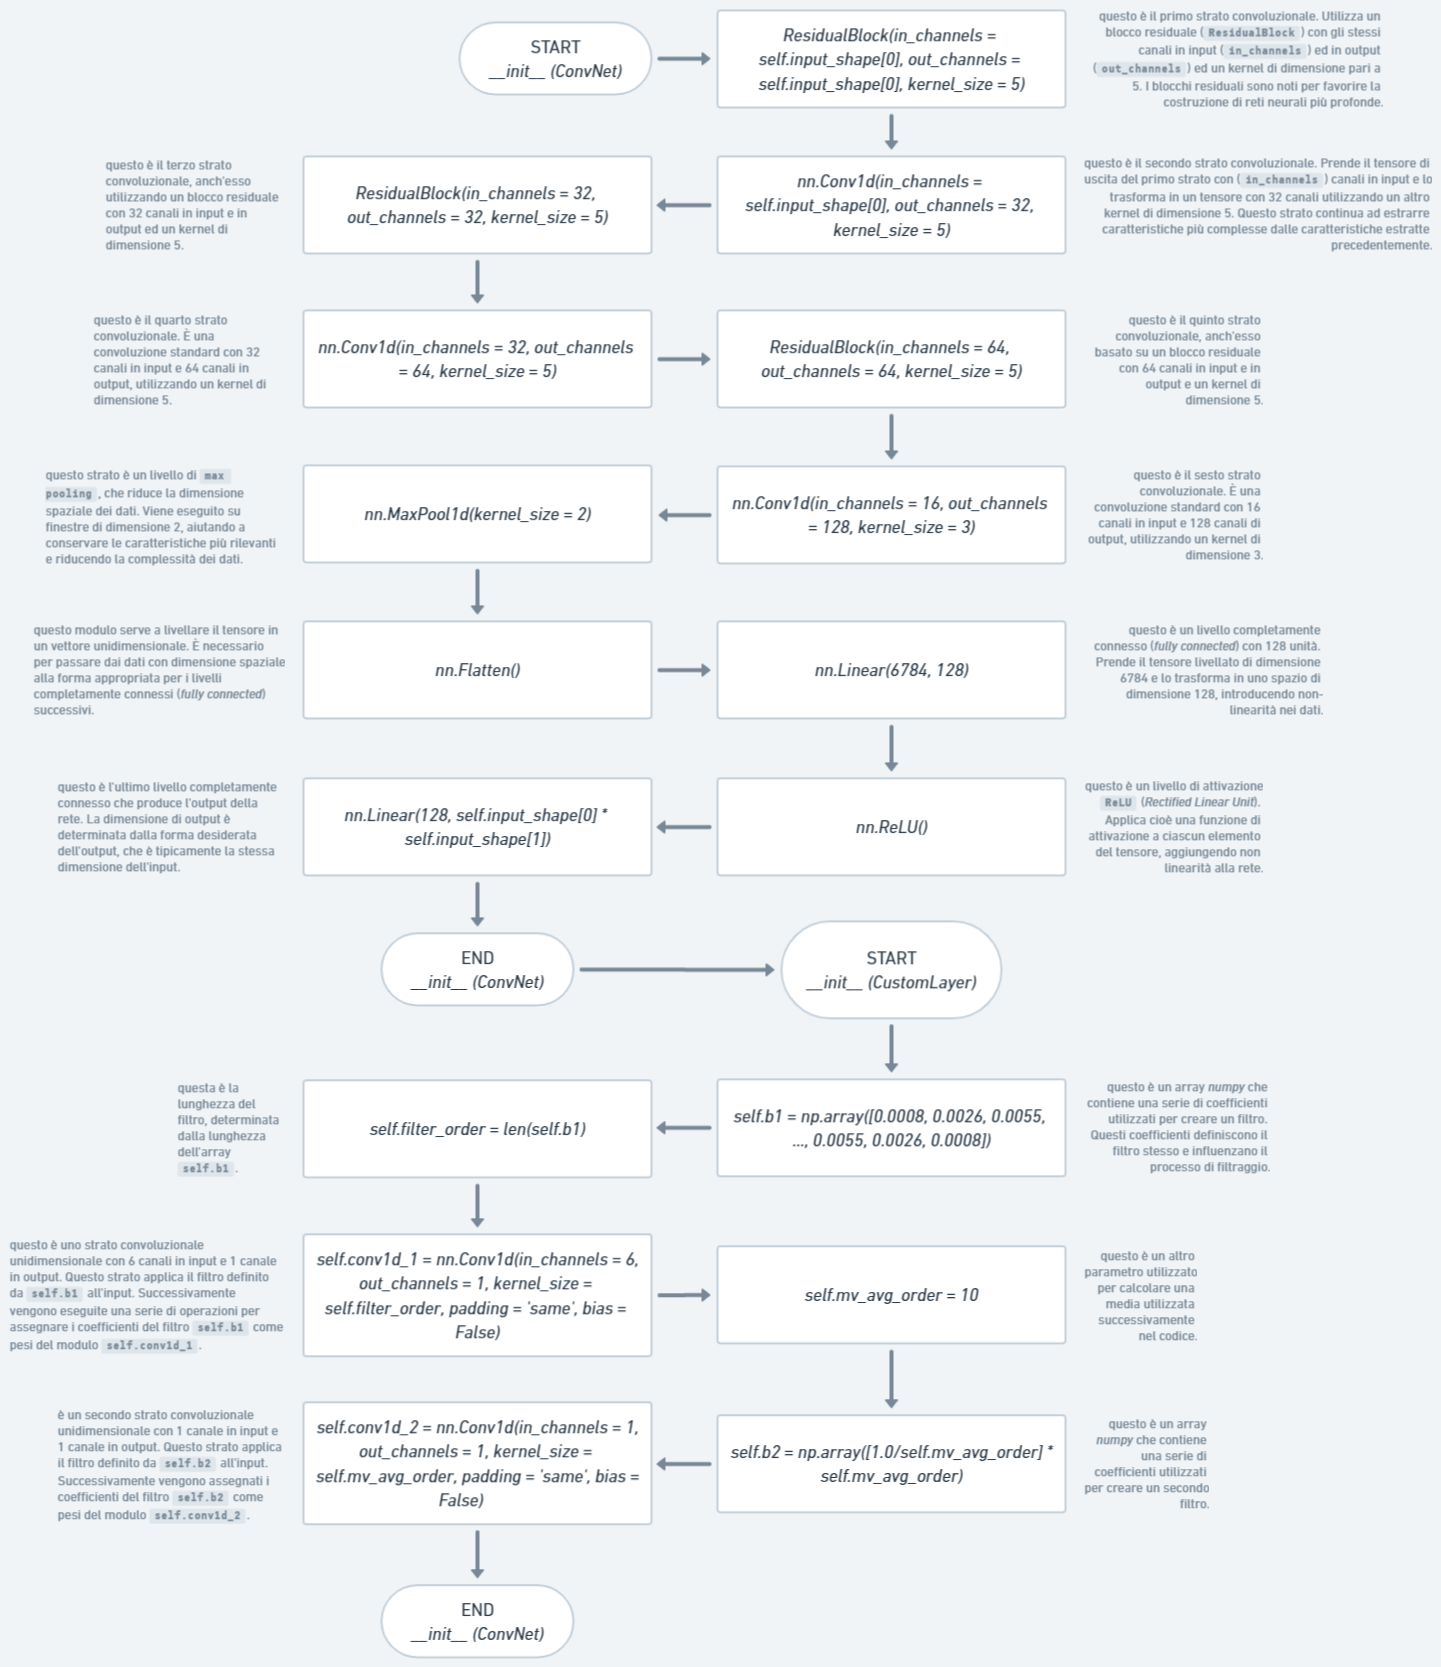
\includegraphics[width=1\textwidth]{immagini/terza.png}
    \captionsetup{justification=centering}
    \caption{Rappresentazione del codice della terza CNN come diagramma di flusso.}
    \label{fig:terza}
\end{figure}

Questa particolare CNN implementa un \textit{Custom Layer} denominato \textit{Final Custom Layer} che include una \textit{ConvNet} ed un ulteriore \textit{Custom Layer}. Il codice della \textit{ConvNet} è formato esattamente come per la precedente CNN implementata, mentre il codice del \textit{Custom Layer} invece, oltre alla definizione delle funzione \texttt{init()} e \texttt{forward()}, include altre tre definizioni di funzioni che, in ordine di apparizione, sono \texttt{pan\_tompkins()}, \texttt{avg\_beat()} e \texttt{spread()}. La funzione \texttt{pan\_tompkins()} è stata sviluppata per rilevare picchi di complessi \textit{QRS} negli ECG dopo che questi sono passati attraverso i vari layer convoluzionali, come se fosse una fase di \textit{post-processing}. La funzione \texttt{avg\_beat()} invece è stata sviluppata con l'obiettivo di calcolare una rappresentazione media dei picchi di complessi \textit{QRS} all'interno di un segmento per ogni ECG. Infine la funzione \texttt{spread()} è stata sviluppata per ottenere il battito medio in modo da posizionarlo nelle corrette posizioni nei successivi sei secondi da predire. Per esempio, si utilizzano le posizioni dei battiti registrate dai \textit{lead} [$ V_{1}, V_{2}, V_{3}, V_{4}, V_{5}, V_{6} $] per stimare la posizione dei battiti nei successivi sei secondi. Questa stima si ottiene prendendo il battito medio dai \textit{lead} [$ I, II, III, aV_{R}, aV_{L}, aV_{F} $], e duplicandolo nei sei secondi successivi. Questa copia avviene per mezzo della funziona di cross-correlazione tra due segnali, dove il primo segnale rappresenta il battito medio mentre il secondo segnale rappresenta quello generato dalla funzione \texttt{pan\_tompkins()}. Nel caso in cui quest'ultimo fosse un impulso perfetto, allora il battito verrebbe copiato totalmente alla posizione dell'impulso.

\section{Addestramento della CNN}
\label{sec:addestramento}

Tutte le CNN implementate durante la ricerca sono state addestrate secondo la stessa logica, in base alla quale sono stati utilizzati due \texttt{DataLoader}, uno per quanto riguarda il \textit{training} del dataset, e l'altro per quanto riguarda invece la \textit{validation} del dataset.

Per tutte le CNN addestrate sono stati impostati ed utilizzati i medesimi parametri, ovvero i valori di \texttt{BATCH\_SIZE} e di \texttt{LEARNING\_RATE} pari a \texttt{16} ed a \texttt{0.001} rispettivamente. Tali parametri sono fondamentali per il corretto funzionamento dell'intera CNN ed indicano rispettivamente il numero di campioni di dati che vengono utilizzati in ogni iterazione di addestramento e la quantità che controlla quanto velocemente la CNN si adatta ai dati dell'addestramento stesso. Inoltre il valore di \texttt{NUM\_EPOCHS}, ovvero il numero di epoche dell'addestramento, è stato impostato pari a \texttt{100}, e l'\textit{optimizer} utilizzato è stato individuato in \texttt{torch.optim.Adam}, cioè un algoritmo di ottimizzazione che combina concetti di ottimizzatori stocastici, ovvero operanti con un certo grado di casualità o aleatorietà, con metodi di adattamento del tasso di apprendimento, rendendolo efficace nella convergenza delle CNN.

In particolare, l'utilizzo di un \texttt{BATCH\_SIZE} più grande può consentire di sfruttare meglio le risorse computazionali ed accelerare l'addestramento della CNN, ma richiede anche una maggiore memoria. D'altra parte, un valore di \texttt{BATCH\_SIZE} più piccolo può essere vantaggioso in termini di utilizzo efficiente della memoria e di generalizzazione della CNN, ma può richiedere più tempo per l'addestramento complessivo. Questa nozione vale anche per il valore di \texttt{LEARNING\_RATE}, infatti un \texttt{LEARNING\_RATE} più alto implica un adattamento più rapido, ma potrebbe anche portare ad oscillazioni o ad un'approssimazione subottimale della soluzione. Al contrario, un valore di \texttt{LEARNING\_RATE} più basso rende l'adattamento più lento, ma potrebbe consentire una migliore convergenza verso una soluzione ottimale. In ogni caso, trovare il giusto valore del \texttt{LEARNING\_RATE} è importante per un addestramento efficace della CNN. Un \texttt{LEARNING\_RATE} troppo alto potrebbe causarne un periodo di instabilità, mentre un \texttt{LEARNING\_RATE} troppo basso potrebbe rallentarne l'addestramento o far sì che la CNN converga verso un minimo locale anziché verso il minimo globale.

In conclusione, si può dedurre che la scelta dei valori di \texttt{BATCH\_SIZE} e di \texttt{LEARNING\_RATE} dipenda dal dataset, dalle risorse computazionali disponibili e dai requisiti specifici del problema. È dunque una pratica molto comune sperimentare diversi valori di \texttt{BATCH\_SIZE} e di \texttt{LEARNING\_RATE} per trovare quelli ottimali per il proprio scenario.

Lo snippet \ref{snippet:addestramento} riportato di seguito rappresenta il codice della funzione utilizzata per l'addestramento delle CNN implementate:

\lstset{language=Python}
\begin{lstlisting}[aboveskip=15pt, belowskip=15pt, basicstyle=\fontsize{8}{10}\selectfont, keywordstyle=\color{blue}, breaklines=true, label=snippet:addestramento]
list_train_loss = []
list_val_loss =  []
def TrainingModel(model, train_loader, val_loader, loss_fn, optimizer, num_epochs):
    global list_train_loss, list_val_loss
    best_loss = float('inf')
    for epoch in range(num_epochs):
        model.train()
        train_loss = 0.0
        for ecgs, targets in train_loader:
            optimizer.zero_grad()
            outputs = model(ecgs.to(device))
            targets = targets.to(device)
            loss = loss_fn(outputs.float(), targets.float())
            train_loss += loss.item()
            loss.backward()
            optimizer.step()
        avg_train_loss = train_loss / len(train_loader)
        list_train_loss.append(avg_train_loss)
        avg_val_loss = EvaluateModel(model, val_loader, loss_fn)
        list_val_loss.append(avg_val_loss)
        print(f'Epoch {epoch + 1}/{num_epochs}: train_loss = {avg_train_loss: .4f}, val_loss = {avg_val_loss: .4f}')
        with open(f'{OUTPUTS_DIRECTORY}/epochs.txt', 'a') as file:
            file.write(f'Epoch {epoch + 1}/{num_epochs}: train_loss = {avg_train_loss: .4f}, val_loss = {avg_val_loss: .4f}\n')
        if avg_val_loss < best_loss:
            best_loss = avg_val_loss
            torch.save(model.state_dict(), 'best_model.pt')
\end{lstlisting}

\section{Validazione della CNN}
\label{sec:validazione}

Il processo di validazione è stato eseguito definendo una funzione che se ne occupasse in maniera esclusiva, in modo da poter calcolare il numero totale di errori ottenuti durante la valutazione stessa, utile successivamente per calcolarne la media rispetto al valore totale di \texttt{BATCH\_SIZE}.

È inoltre di fondamentale importanza il parametro \texttt{LOSS\_FN} che viene passato in input alla funzione, e che è la componente che si occupa effettivamente del calcolo degli errori tra le predizioni ed i target. Viene definita precedentemente nel codice come \texttt{loss = nn.MSELoss()} e viene di solito utilizzata in problemi di regressione, in cui l'obiettivo è predire un valore numerico continuo. La funzione \texttt{MSE}, abbreviazione di \textit{Mean Squared Error}, calcola la differenza al quadrato tra ogni elemento delle predizioni e dei target e ne calcola infine la media.

In sintesi, questa funzione valuta la CNN utilizzando il \texttt{DataLoader} di validazione fornito. Itera attraverso i \texttt{BATCH} di dati, passa i dati attraverso la CNN per ottenerne le predizioni, calcola l'errore tra queste ed i target, ed infine calcola la media della perdita su tutti i \texttt{BATCH} di dati. Ciò fornisce una stima dell'errore della CNN durante la fase di validazione.

Lo snippet \ref{snippet:validazione} riportato di seguito rappresenta il codice della funzione utilizzata per la validazione delle CNN implementate:

\lstset{language=Python}
\begin{lstlisting}[aboveskip=15pt, belowskip=15pt, basicstyle=\fontsize{8}{10}\selectfont, keywordstyle=\color{blue}, breaklines=true, label=snippet:validazione]
def EvaluateModel(model, loader, loss_fn):
    model.eval()
    total_loss = 0.0
    with torch.no_grad():
        for values in loader:
            ecgs = values[0]
            targets = values[1]
            outputs = model(ecgs.to(device))
            targets = targets.to(device)
            loss = loss_fn(outputs.float(), targets.float())
            total_loss += loss.item()
    avg_loss = total_loss / len(loader)
    return avg_loss
\end{lstlisting}

\section{Analisi di clustering applicata ai segnali}
\label{sec:clustering}

Dopo aver appurato le scarse prestazioni in termini di risultati delle CNN implementate e testate, è stata imboccata una strada per provare a semplificare i dati su cui effettuare l'addestramento delle reti, utilizzando l'algoritmo di clustering \textit{K-means}, utilizzato nell'apprendimento automatico e nell'analisi dei dati per raggruppare dati simili in insiemi comunemente chiamati \textit{cluster}. L'obiettivo principale dell'algoritmo è dunque di suddividere un iniziale insieme di dati in diversi \textit{cluster}, in modo che i dati all'interno dello stesso \textit{cluster} siano simili tra loro ed i dati in \textit{cluster} diversi siano diversi~\cite{cluster}. In questa maniera, idealmente le CNN implementate dovrebbero riuscire ad operare meglio sui segnali, vista la similarità tra gli stessi pur mantenendo un elevato numero di dati totale, fondamentale per l'addestramento.

Lo snippet \ref{snippet:clustering} riportato di seguito rappresenta il codice delle due funzioni utilizzate per effettuare l'analisi di clustering:

\lstset{language=Python}
\begin{lstlisting}[aboveskip=15pt, belowskip=15pt, basicstyle=\fontsize{8}{10}\selectfont, keywordstyle=\color{blue}, breaklines=true, label=snippet:clustering]
def CalculateFeatures(frank_ecg, all_features, index):
    mean_values = torch.mean(frank_ecg, dim = 1)
    std_values = torch.std(frank_ecg, dim = 1)
    rms_values = torch.sqrt(torch.mean(torch.square(frank_ecg), dim = 1))
    mean_diff_values = torch.mean(torch.diff(frank_ecg, dim = 1), dim = 1)
    skewness_values = torch.tensor([skew(col.numpy()) for col in frank_ecg])
    kurtosis_values = torch.tensor([kurtosis(col.numpy()) for col in frank_ecg])
    all_features[index] = torch.cat([mean_values, std_values, rms_values, mean_diff_values, skewness_values, kurtosis_values])
    return all_features

def CalculateKMeans(all_features, ecgs_features, do_plot = False):
    cluster_labels = np.zeros(all_features.shape[0])
    kmeans = KMeans(n_clusters = 10, random_state = 15)
    kmeans.fit(all_features)
    cluster_labels = kmeans.labels_
    unique_labels = np.unique(cluster_labels)
    label_counts = [(label, np.count_nonzero(cluster_labels == label)) for label in unique_labels]
    sorted_labels = sorted(label_counts, key = lambda x: x[1], reverse = True)
    if do_plot:
        for label, count in sorted_labels:
            print(f'Etichetta {label:.0f}: {count}')
    clusters = {}
    for i, cluster in enumerate(cluster_labels):
        if cluster not in clusters:
            clusters[cluster] = []
        clusters[cluster].append(all_features[i])
    sorted_clusters = sorted(clusters.items(), key = lambda x: len(x[1]), reverse = True)
    max_cluster = sorted_clusters[0][1]
    frank_ecgs = []
    for i in ecgs_features:
        for j in max_cluster:
            if((list(i.values())[0] == j).all()):
                frank_ecgs.append(list(i.keys())[0])
    if do_plot:
        tot = 0
        for cluster, ecg_list in sorted_clusters:
            print(f'Cluster {cluster}:')
            print(len(ecg_list))
            tot += len(ecg_list)
            for ecg in ecg_list:
                print(ecg)
            print()
            plt.figure()
            plt.plot(ecg_list[0])
            plt.title(f'Cluster {cluster}')
            plt.show()
        print(tot)
        for i in frank_ecgs[: 5]:
            lead_x = i[0]
            lead_y = i[1]
            lead_z = i[2]
            fig = plt.figure()
            ax = fig.add_subplot(projection = '3d')
            ax.scatter(lead_x, lead_y, lead_z)
            ax.set_title(f'ECG 3D () - Lead X, Y, Z')
            ax.set_xlabel('Lead X')
            ax.set_ylabel('Lead Y')
            ax.set_zlabel('Lead Z')
            plt.show()
    return frank_ecgs
\end{lstlisting}

La prima funzione, chiamata \texttt{CalculateFeatures}, è stata progettata per calcolare diverse \textit{features}, ovvero diverse metriche lungo l'asse delle colonne e cioè lungo la dimensione uno, per ognuno dei segnali di Frank, tra le quali: il valore medio, la deviazione standard, il valore quadratico medio, la media delle differenze tra i punti adiacenti lungo l'asse, l'asimmetria del segnale stesso e la curtosi, cioè un allontanamento dalla normalità distributiva, rispetto alla quale si verifica un maggiore appiattimento o un maggiore allungamento, sempre relativo al segnale stesso. Il calcolo di tutte queste \textit{features} è necessario per il corretto funzionamento dell'algoritmo di clustering implementato successivamente.

La seconda funzione, chiamata invece \texttt{CalculateKMeans}, è stata progettata allo scopo di applicare l'algoritmo \textit{K-means}. Una volta calcolate le \textit{features}, l'obiettivo è stato quello di raggruppare i segnali per similarità in dieci \textit{cluster}, ordinarli poi in ordine decrescente in base al numero di segnali contenuti in ciascuno di essi, e salvare infine solo i segnali presenti all'interno del primo \textit{cluster}, ovvero idealmente quello contenente il numero maggiore di segnali, in modo da avere un nuovo dataset di dimensione ridotta rispetto all'originale ma costituito esclusivamente da segnali con caratteristiche simili tra loro.

Una volta applicato questo algoritmo ed eseguiti i test, si sono notati evidenti miglioramenti nei risultati ottenuti dall'addestramento delle CNN, nonostante non fossero ancora conformi alle aspettative ed alle previsioni iniziali. Inoltre, anche per quanto riguarda il calcolo dell'entropia, facendo riferimento alla sezione ``Entropia'' (Cap. \ref{chap:materiali} Sez. \ref{sec:entropia}), sono stati osservati visibili miglioramenti dati dal fatto che questa sia stata notevolmente ridotta grazie all'aggregazione dei dati in cluster omogenei. Tutti questi riscontri hanno dunque confermato l'efficacia dell'approccio di clustering nell'organizzazione e nella semplificazione dei dati, contribuendo inoltre ad aumentare generalmente le performance, la qualità e l'accuratezza dei risultati.

\chapter{Risultati e discussione}
\label{chap:risultati}

\section{Entropia}
\label{sec:entropia_risultati}

I valori dell'indice di predicibilità calcolati ed ottenuti pre e post applicazione dell'algoritmo di clustering sono tra loro molto diversi. Ciò è dovuto, come da previsioni, alla semplificazione dei dati del dataset, che in totale sono diventati pari a 1582 ECG, rispetto ai 21799 ECG iniziali. Dunque, il valore dell'indice calcolato a seguito della semplificazione del dataset è pari ad $ h = 0.924 $, mentre il valore dell'indice calcolato utilizzando il dataset prima della semplificazione è pari ad $ h = 0.896 $.

La figura \ref{fig:hists2} riportata di seguito invece, illustra la rappresentazione della matrice contenente la somma delle distribuzioni bidimensionali relative ad ogni battito di tutti gli ECG in seguito alla semplificazione dei dati del dataset:

\begin{figure}[H]
    \centering
    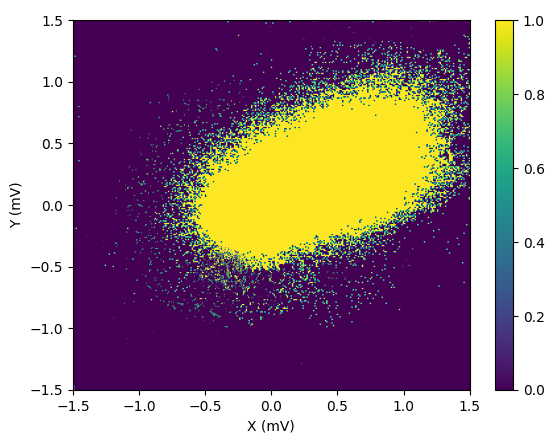
\includegraphics[width=0.65\textwidth]{immagini/hists2.png}
    \captionsetup{justification=centering}
    \caption{Rappresentazione della matrice contenente la somma delle distribuzioni bidimensionali relative ad ogni battito di tutti gli ECG, in seguito alla semplificazione del dataset.}
    \label{fig:hists2}
\end{figure}

Si può dunque notare un miglioramento significativo rispetto alla figura \ref{fig:hists} riportata nella sezione ``Entropia'' (Cap. \ref{chap:materiali} Sez. \ref{sec:entropia}), ottenuto proprio grazie alla semplificazione dei dati del dataset in seguito all'applicazione dell'algoritmo di clustering, confermandone quindi ancor di più l'efficacia e la validità.

\section{Risultati prodotti dalle reti pre-clustering}
\label{sec:network_risultati}

I risultati illustrati di seguito mostrano invece come purtoppo non sia stato possibile ottenere ciò che inizialmente si sperava, nonostante le molte reti neurali implementate e testate. Vengono dunque riportati in termini di figure e relative spiegazioni, relativi a tutte e tre le CNN riportate nella sezione ``Rete neurale convoluzionale'' (Cap. \ref{chap:materiali} Sez. \ref{sec:network}).


\subsection{Prima CNN}
\label{subsec:prima_risultati}

La seguente figura \ref{fig:prima_cnn_primo_plot} illustra la differenze tra le due curve di \textit{train} e \textit{val losses} che rappresentano rispettivamente la misura dell'errore della CNN durante l'addestramento sui dati di addestramento stessi, e la valutazione dell'errore della CNN sui dati di validazione, che invece sono dati separati sui quali la CNN non ha mai avuto modo di operare prima. Di solito, la curva di \textit{train loss} diminuisce costantemente durante l'addestramento poiché la CNN impara dai dati di addestramento. Tuttavia, la curva di \textit{val loss} può comportarsi in modo diverso: se la \textit{val loss} inizia ad aumentare mentre la \textit{train loss} continua a diminuire, è un segno di \textit{overfitting}, il che significa che la CNN sta iniziando ad apprendere il rumore nei dati di addestramento invece di generalizzare correttamente. In generale, le curve di \textit{train} e \textit{val losses} possono guidare la scelta della CNN migliore. L'obiettivo quindi è trovare un equilibrio tra la minimizzazione dell'errore sui dati di addestramento (\textit{train loss} bassa) ed il mantenenimento di un buon livello di generalizzazione sui dati di validazione (\textit{val loss} bassa):

\begin{figure}[H]
    \centering
    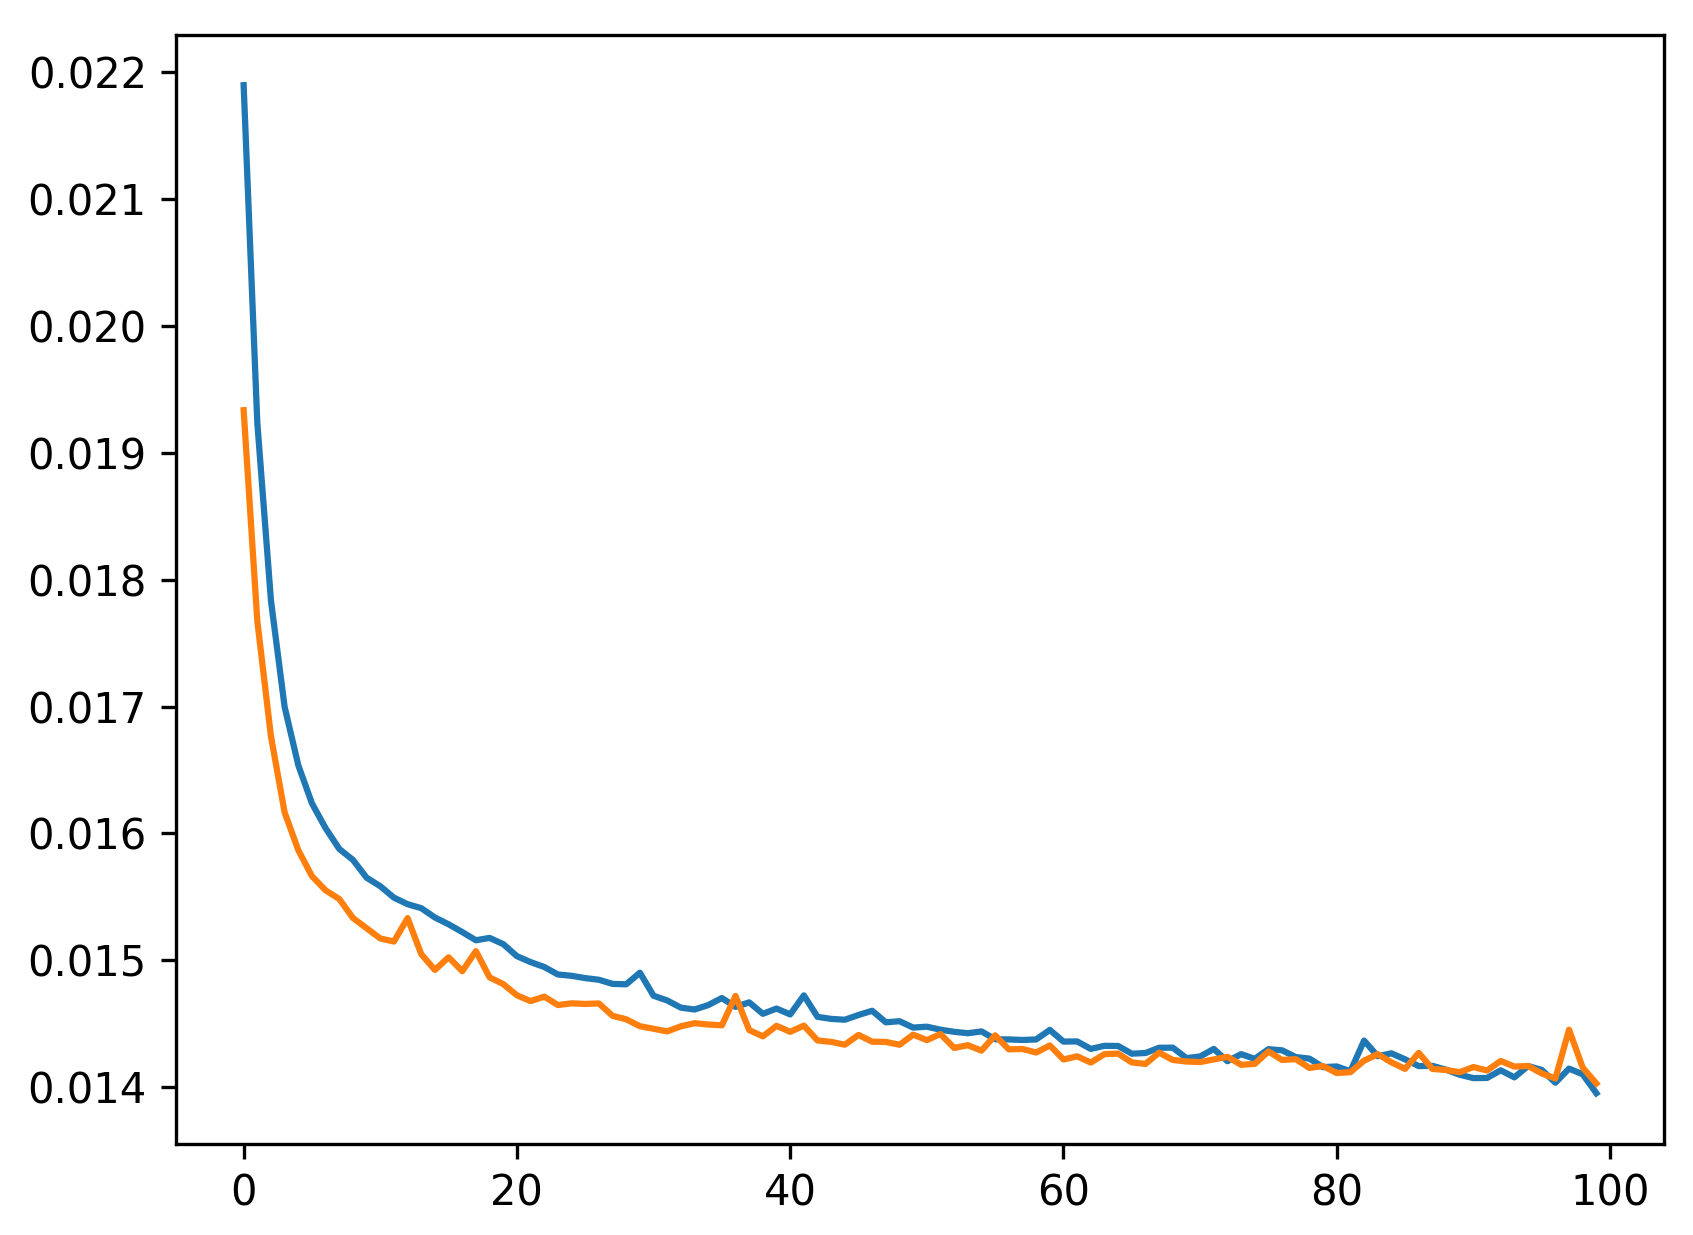
\includegraphics[width=0.65\textwidth]{immagini/prima_cnn_primo_plot.png}
    \captionsetup{justification=centering}
    \caption{Differenze tra le curve di \textit{val loss} (in blu) e \textit{train loss} (in arancione) riferite alla prima CNN implementata e testata.}
    \label{fig:prima_cnn_primo_plot}
\end{figure}

Nonostante le due curve di \textit{train loss} e \textit{val loss} fossero risultate entrambe molto positive poiché entrambe in diminuzione, i \textit{plot} ottenuti una volta completati i test non hanno portato i risultati inizialmente sperati, come si può dedurre dalla seguente figura \ref{fig:prima_cnn_secondo_plot}, che mostra come purtroppo i due grafici non si sovrappongono quasi mai:

\begin{figure}[H]
    \centering
    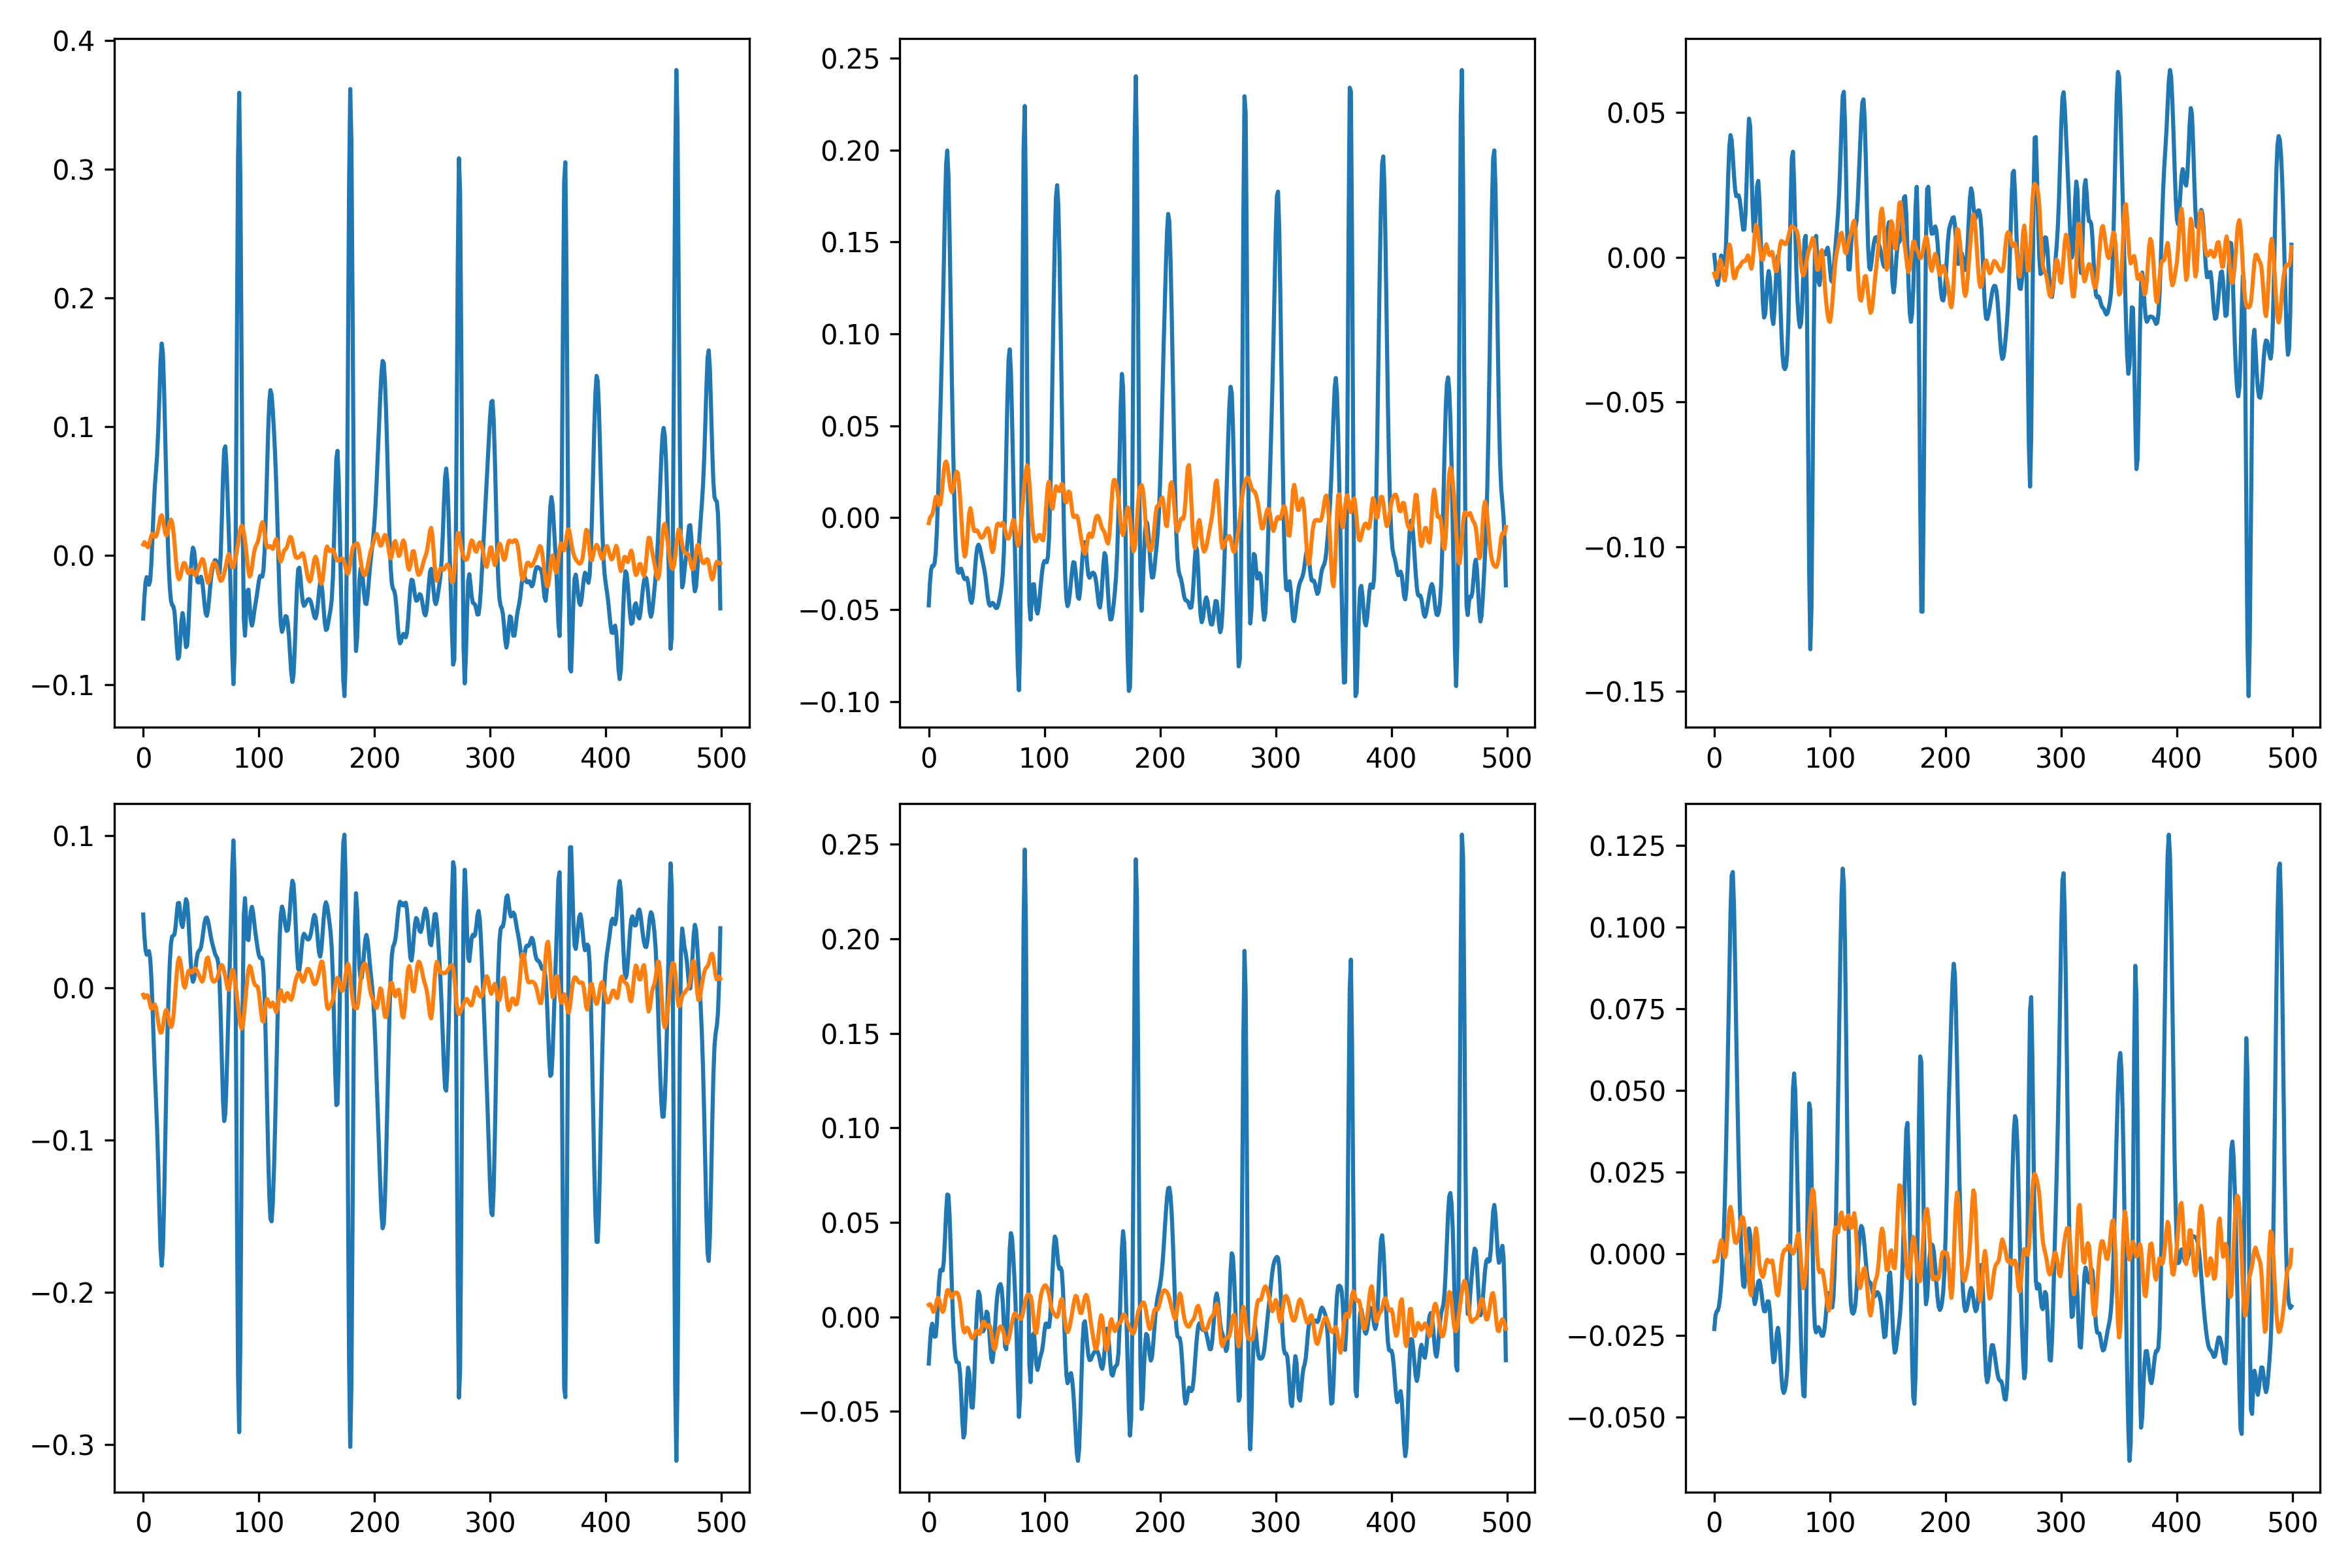
\includegraphics[width=0.85\textwidth]{immagini/prima_cnn_secondo_plot.png}
    \captionsetup{justification=centering}
    \caption{Risultati ottenuti dai test effettuati con la prima CNN implementata e testata.}
    \label{fig:prima_cnn_secondo_plot}
\end{figure}


\subsection{Seconda CNN}
\label{subsec:seconda_risultati}

Come sopra, la seguente figura \ref{fig:seconda_cnn_primo_plot} illustra la differenze tra le due curve di \textit{train} e \textit{val losses} riferite alla CNN immediatamente sopra riporata. Si può notare come, nonostante un incremento di complessità non indifferente della CNN, la curva di \textit{val loss} non sia in diminuzione per tutto il periodo di tempo dell'addestramento, ma soltanto per un primo intervallo di tempo, per poi essere di poco in aumento fino a stabilizzarsi verso la fine attorno ad un certo valore. Ciò dimostra come un incremento della complessità della CNN non implichi necessariamente un miglioramento dei risultati ottenuti dai test, ed anzi spesso ne provochi un grave deterioramento come in questo caso:

\begin{figure}[H]
    \centering
    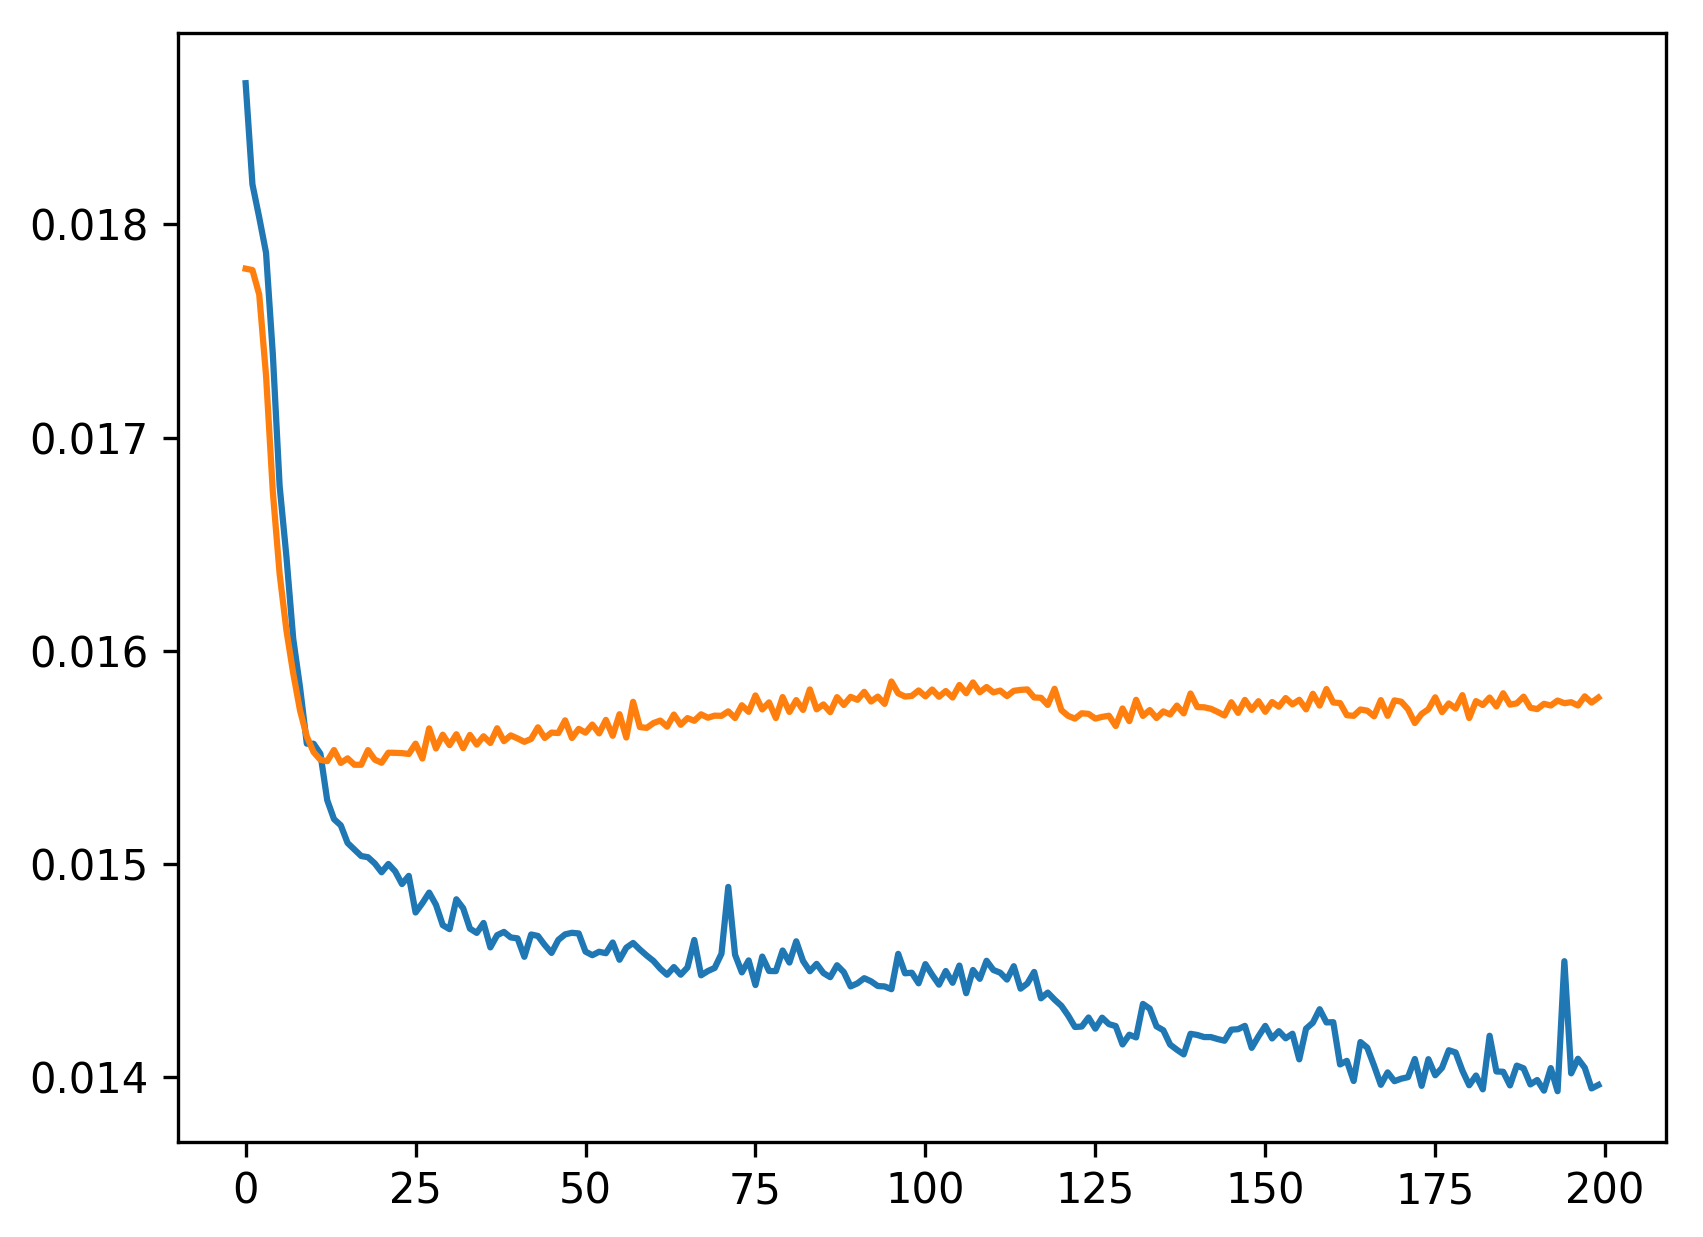
\includegraphics[width=0.65\textwidth]{immagini/seconda_cnn_primo_plot.png}
    \captionsetup{justification=centering}
    \caption{Differenze tra le curve di \textit{val loss} (in blu) e \textit{train loss} (in arancione) riferite alla seconda CNN implementata e testata.}
    \label{fig:seconda_cnn_primo_plot}
\end{figure}

In questo caso, nonostante le due curve di \textit{train} e \textit{val losses} fossero risultate molto peggiori in termini di risultati rispetto alle curve della prima CNN sopra riportate, si può invece notare dalle seguenti figure \ref{fig:seconda_cnn_secondo_plot_0} e \ref{fig:seconda_cnn_secondo_plot_1} come i \textit{plot} ottenuti una volta terminati i test abbiano portato risultati molto più vicini a ciò che ci si aspetterebbe rispetto ai \textit{plot} ottenuti dai test della prima CNN, nonostante ancora una volta non siano comunque soddisfacenti in termini di risultati, il che ha dunque portato a modificare nuovamente la CNN alla ricerca di risultati migliori:

\begin{figure}[H]
    \centering
    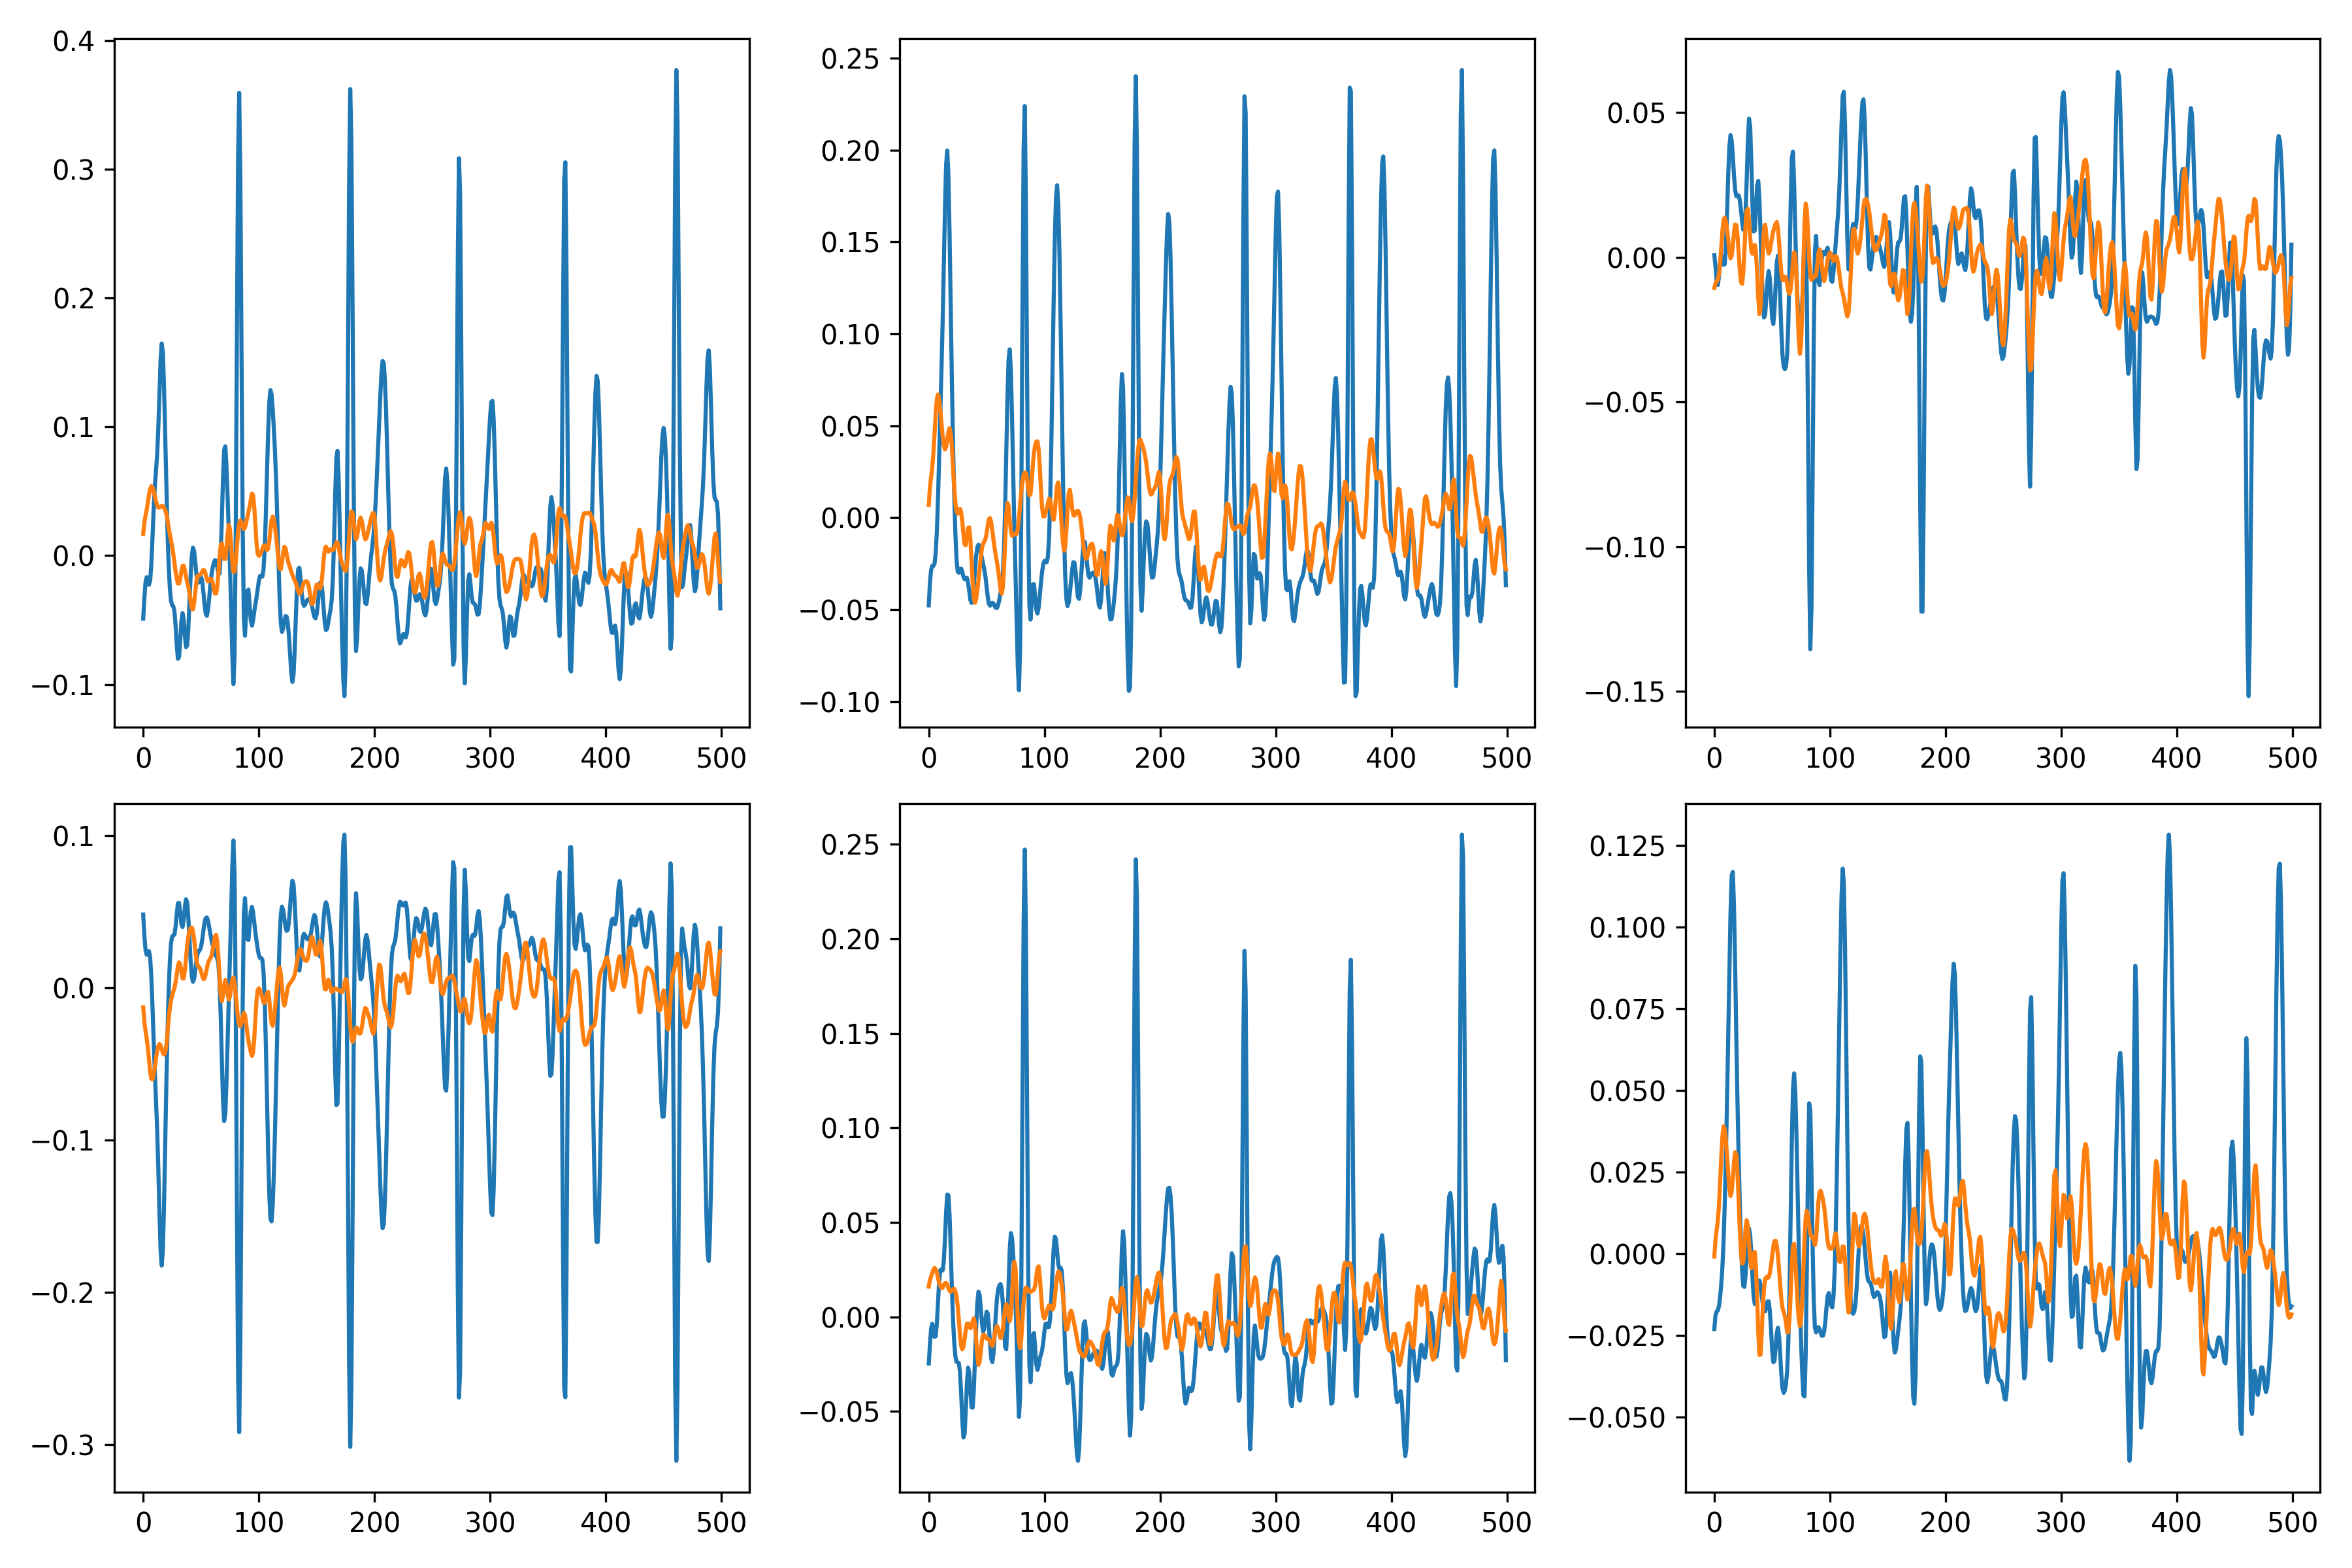
\includegraphics[width=0.85\textwidth]{immagini/seconda_cnn_secondo_plot_0.png}
    \captionsetup{justification=centering}
    \caption{Risultati ottenuti dai test effettuati con la seconda CNN implementata e testata.}
    \label{fig:seconda_cnn_secondo_plot_0}
\end{figure}
\begin{figure}[H]
    \centering
    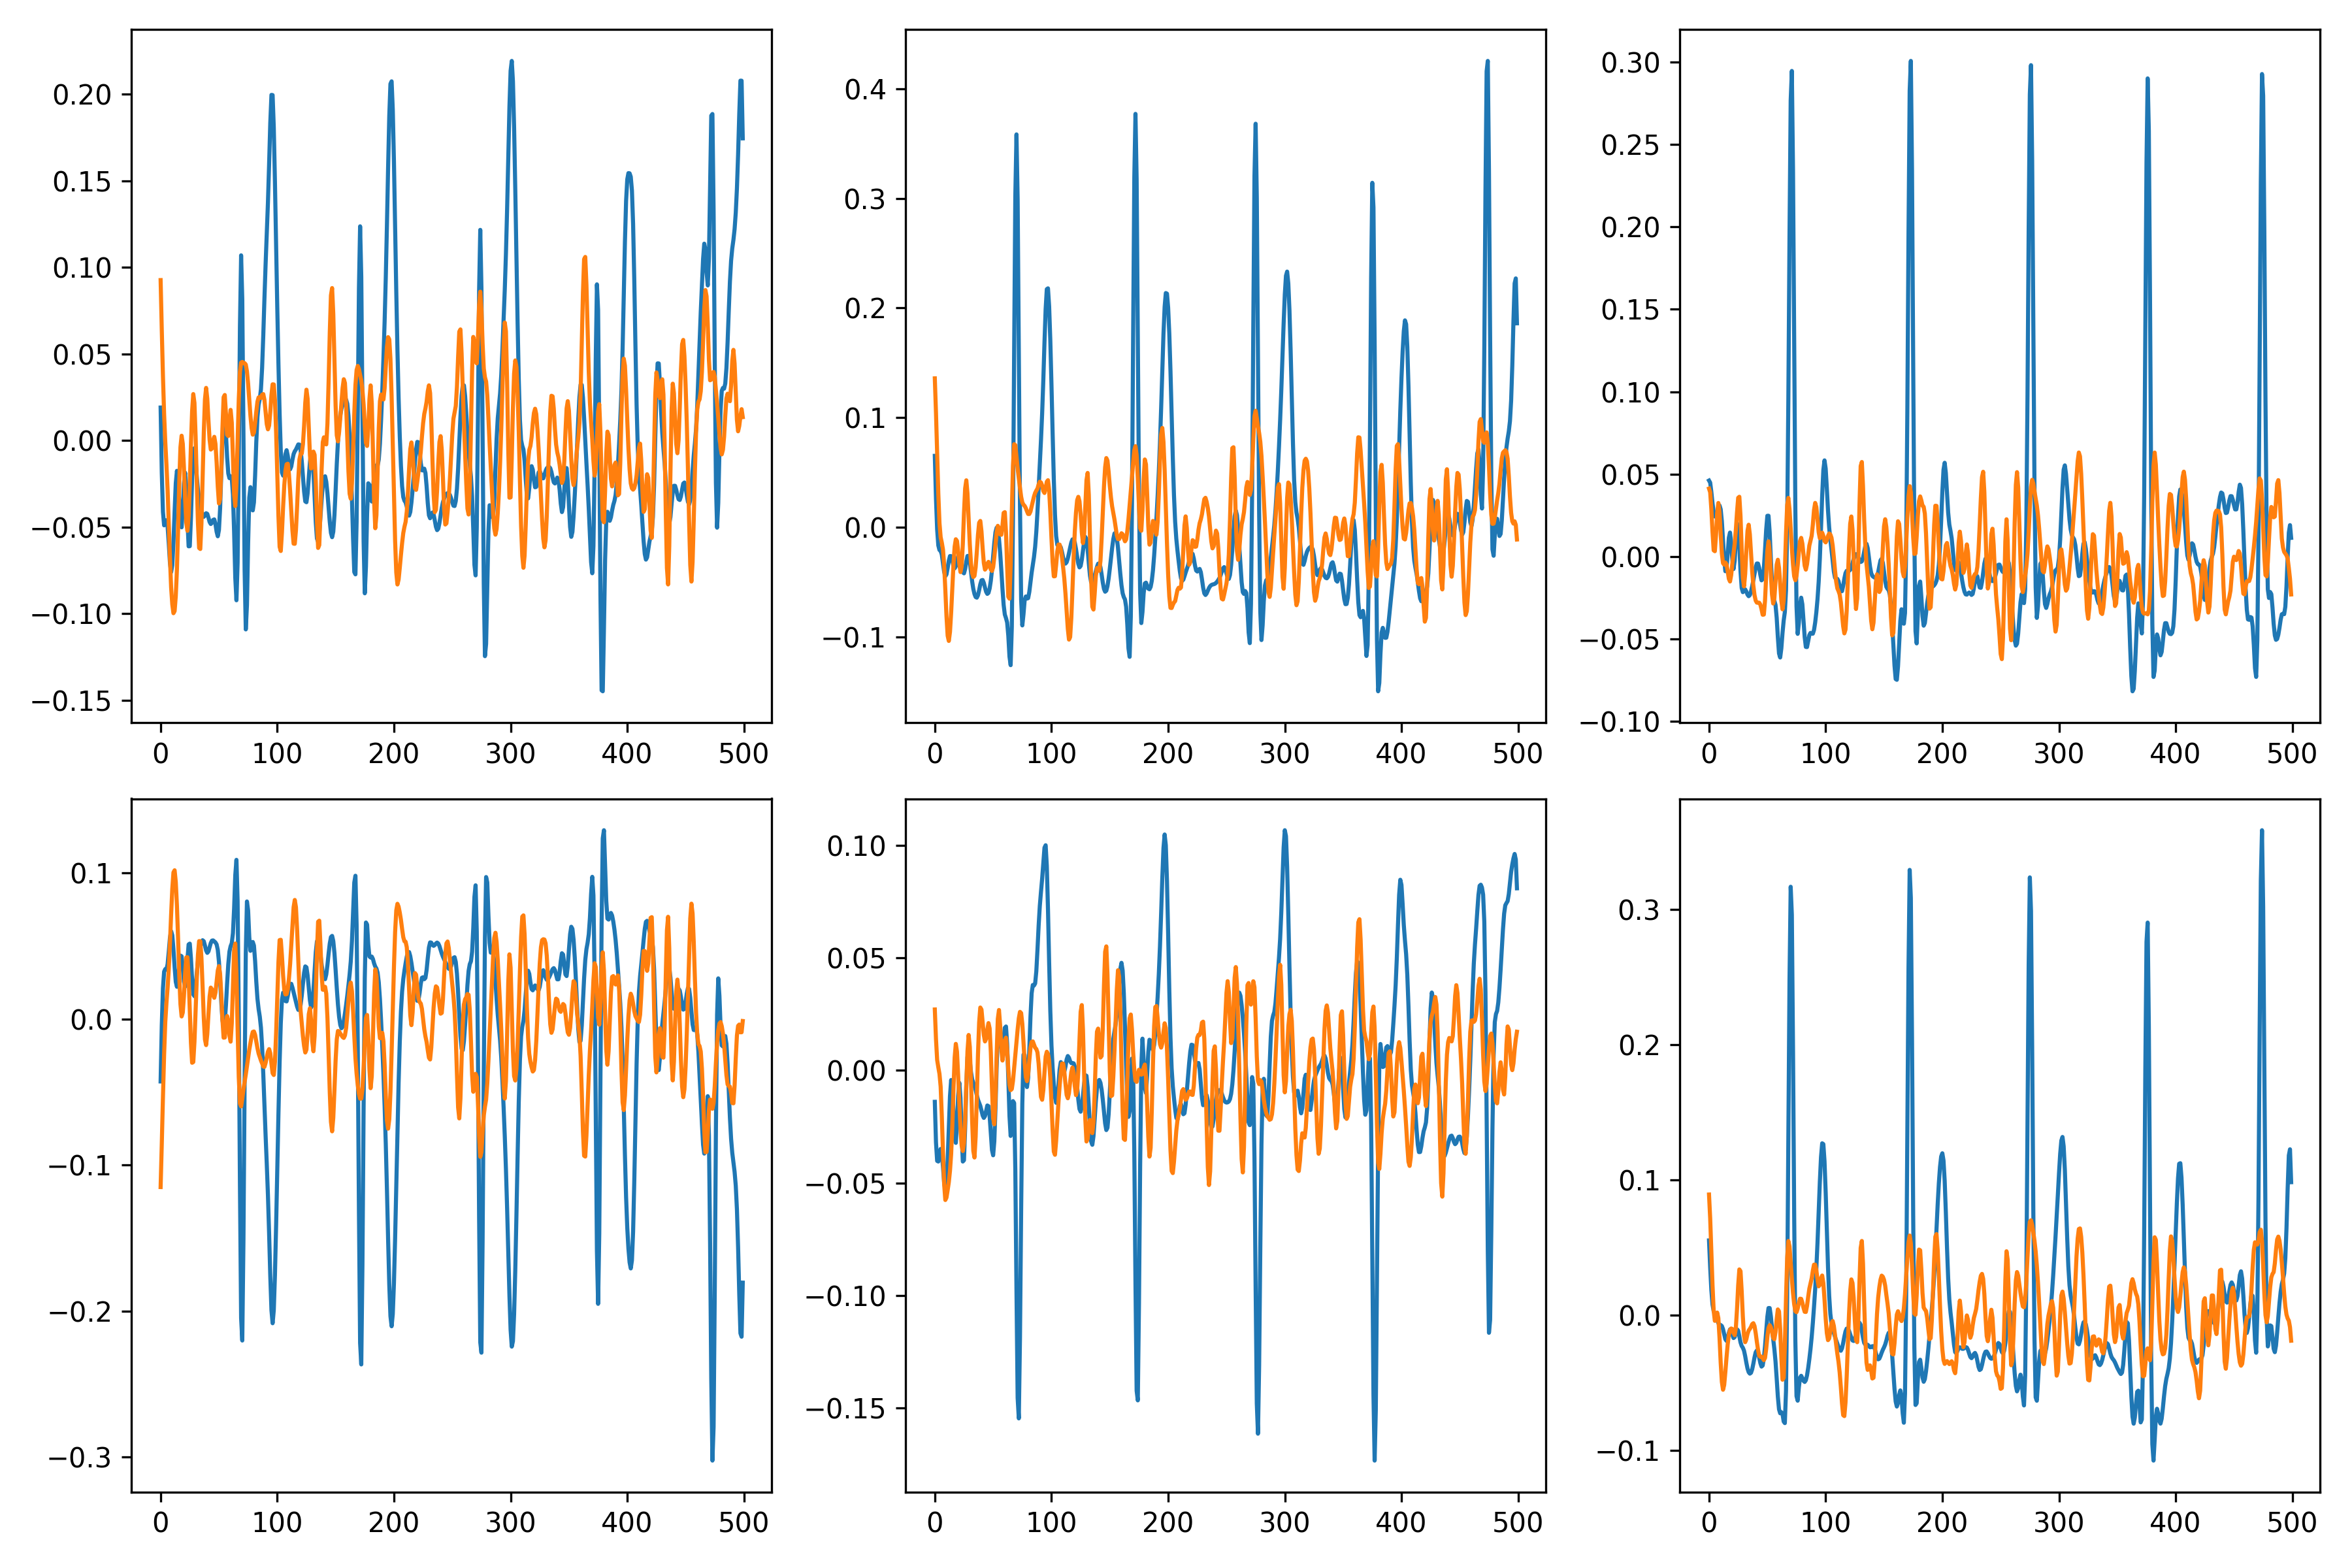
\includegraphics[width=0.85\textwidth]{immagini/seconda_cnn_secondo_plot_1.png}
    \captionsetup{justification=centering}
    \caption{Risultati ottenuti dai test effettuati con la seconda CNN implementata e testata.}
    \label{fig:seconda_cnn_secondo_plot_1}
\end{figure}


\subsection{Terza CNN}
\label{subsec:terza_risultati}

Infine, di seguito viene riportata l'ultima figura \ref{fig:terza_cnn_primo_plot} che illustra la differenze tra le due curve di \textit{train} e \textit{val losses} riferite alla CNN immediatamente sopra riporata. In questo caso entrambe le curve sono in diminuzione in un primo intervallo temporale, fino a che non si stabilizzano rimanendo quasi del tutto al medesimo valore fino al termine dei test, anche se si nota un aumento molto ripido seguito immediatamente da un'ulteriore diminuzione altrettanto ripida verso la conclusione dei test sull'asse temporale delle ascisse, da parte della curva di \textit{train loss}:

\begin{figure}[H]
    \centering
    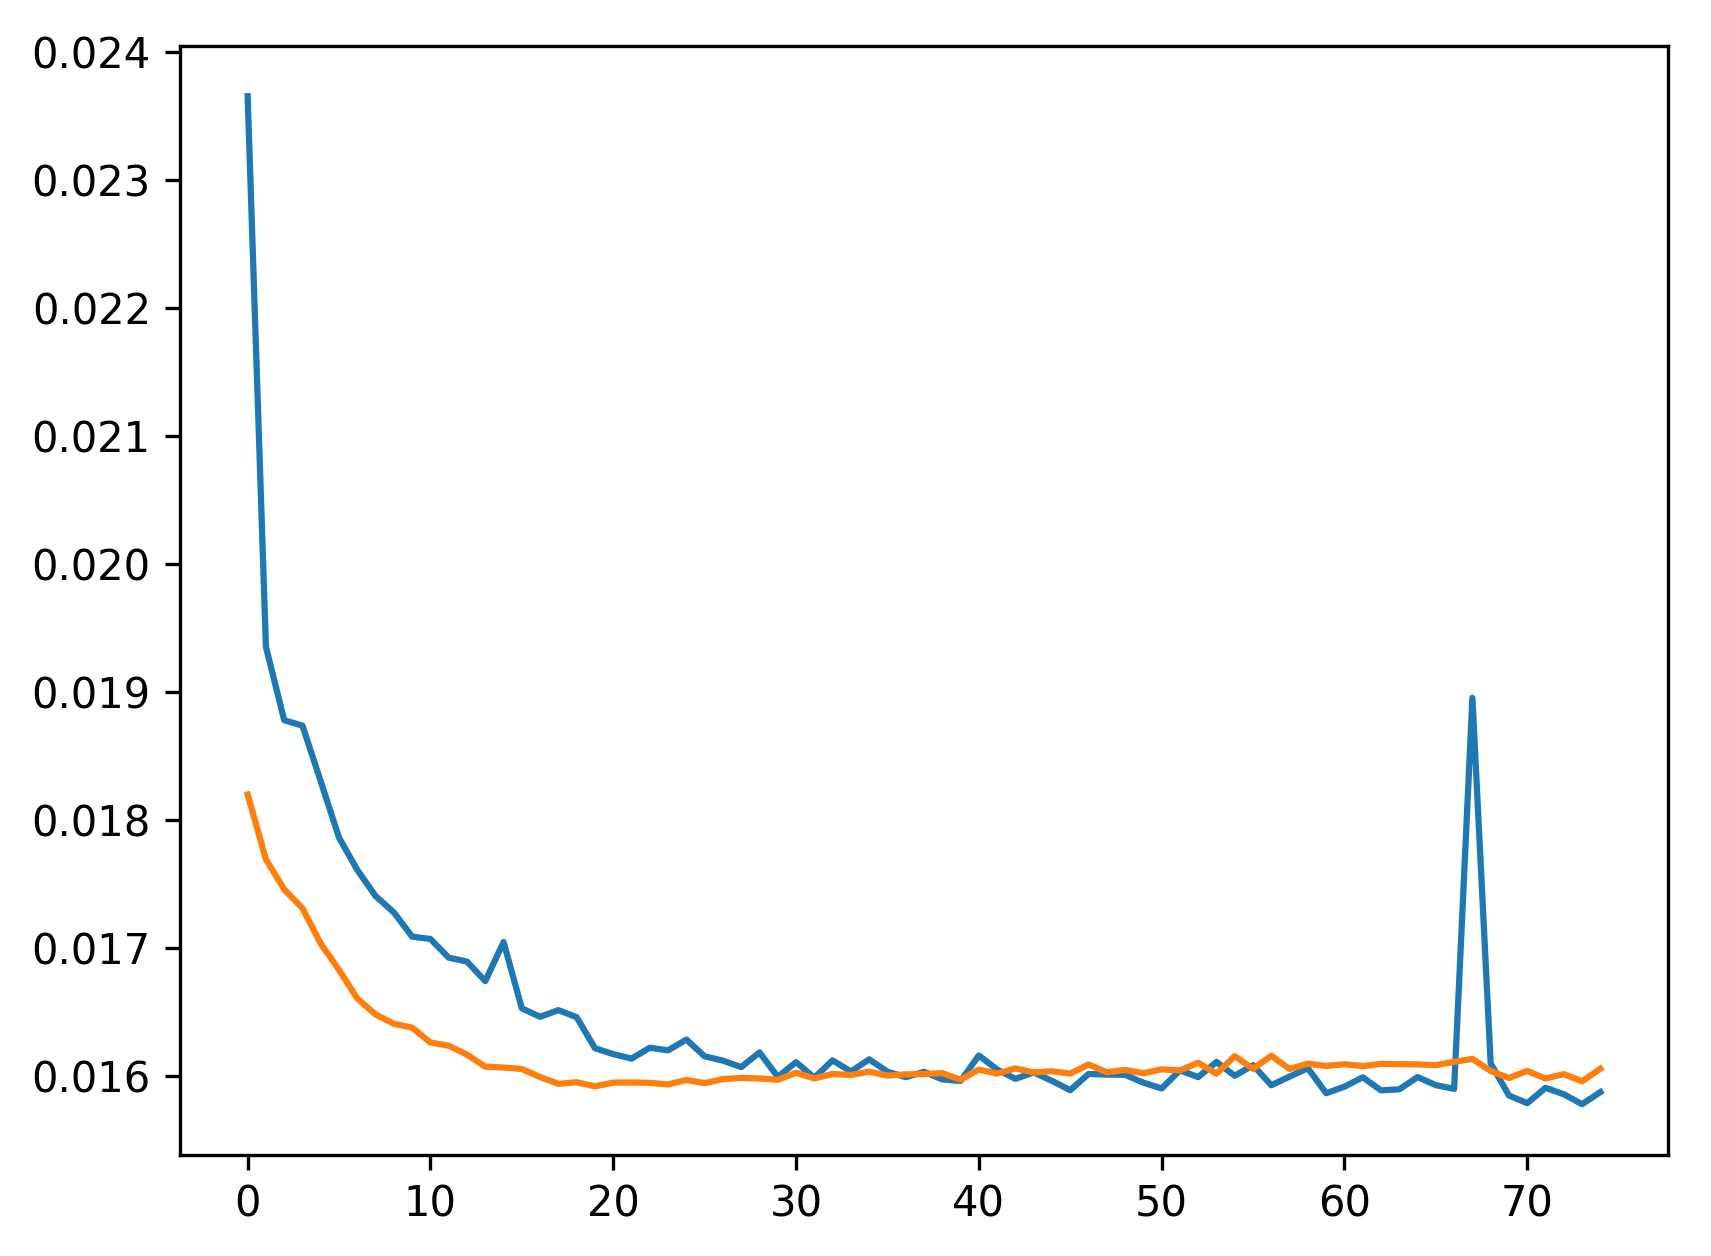
\includegraphics[width=0.65\textwidth]{immagini/terza_cnn_primo_plot.png}
    \captionsetup{justification=centering}
    \caption{Differenze tra le curve di \textit{val loss} (in blu) e \textit{train loss} (in arancione) riferite alla terza CNN implementata e testata.}
    \label{fig:terza_cnn_primo_plot}
\end{figure}

Dunque avendo visionato le due curve di \textit{train} e \textit{val losses}, si può notare dalle seguenti figure \ref{fig:terza_cnn_secondo_plot_0} e \ref{fig:terza_cnn_secondo_plot_1} come i \textit{plot} ottenuti una volta conclusi i test abbiano portato a risultati ancora una volta molto vicini a ciò che ci si aspetterebbe, essendo le linee sovrapposte in molteplici punti, nonostante purtroppo ancora una volta non siano comunque completamente soddisfacenti in termini di risultati:

\begin{figure}[H]
    \centering
    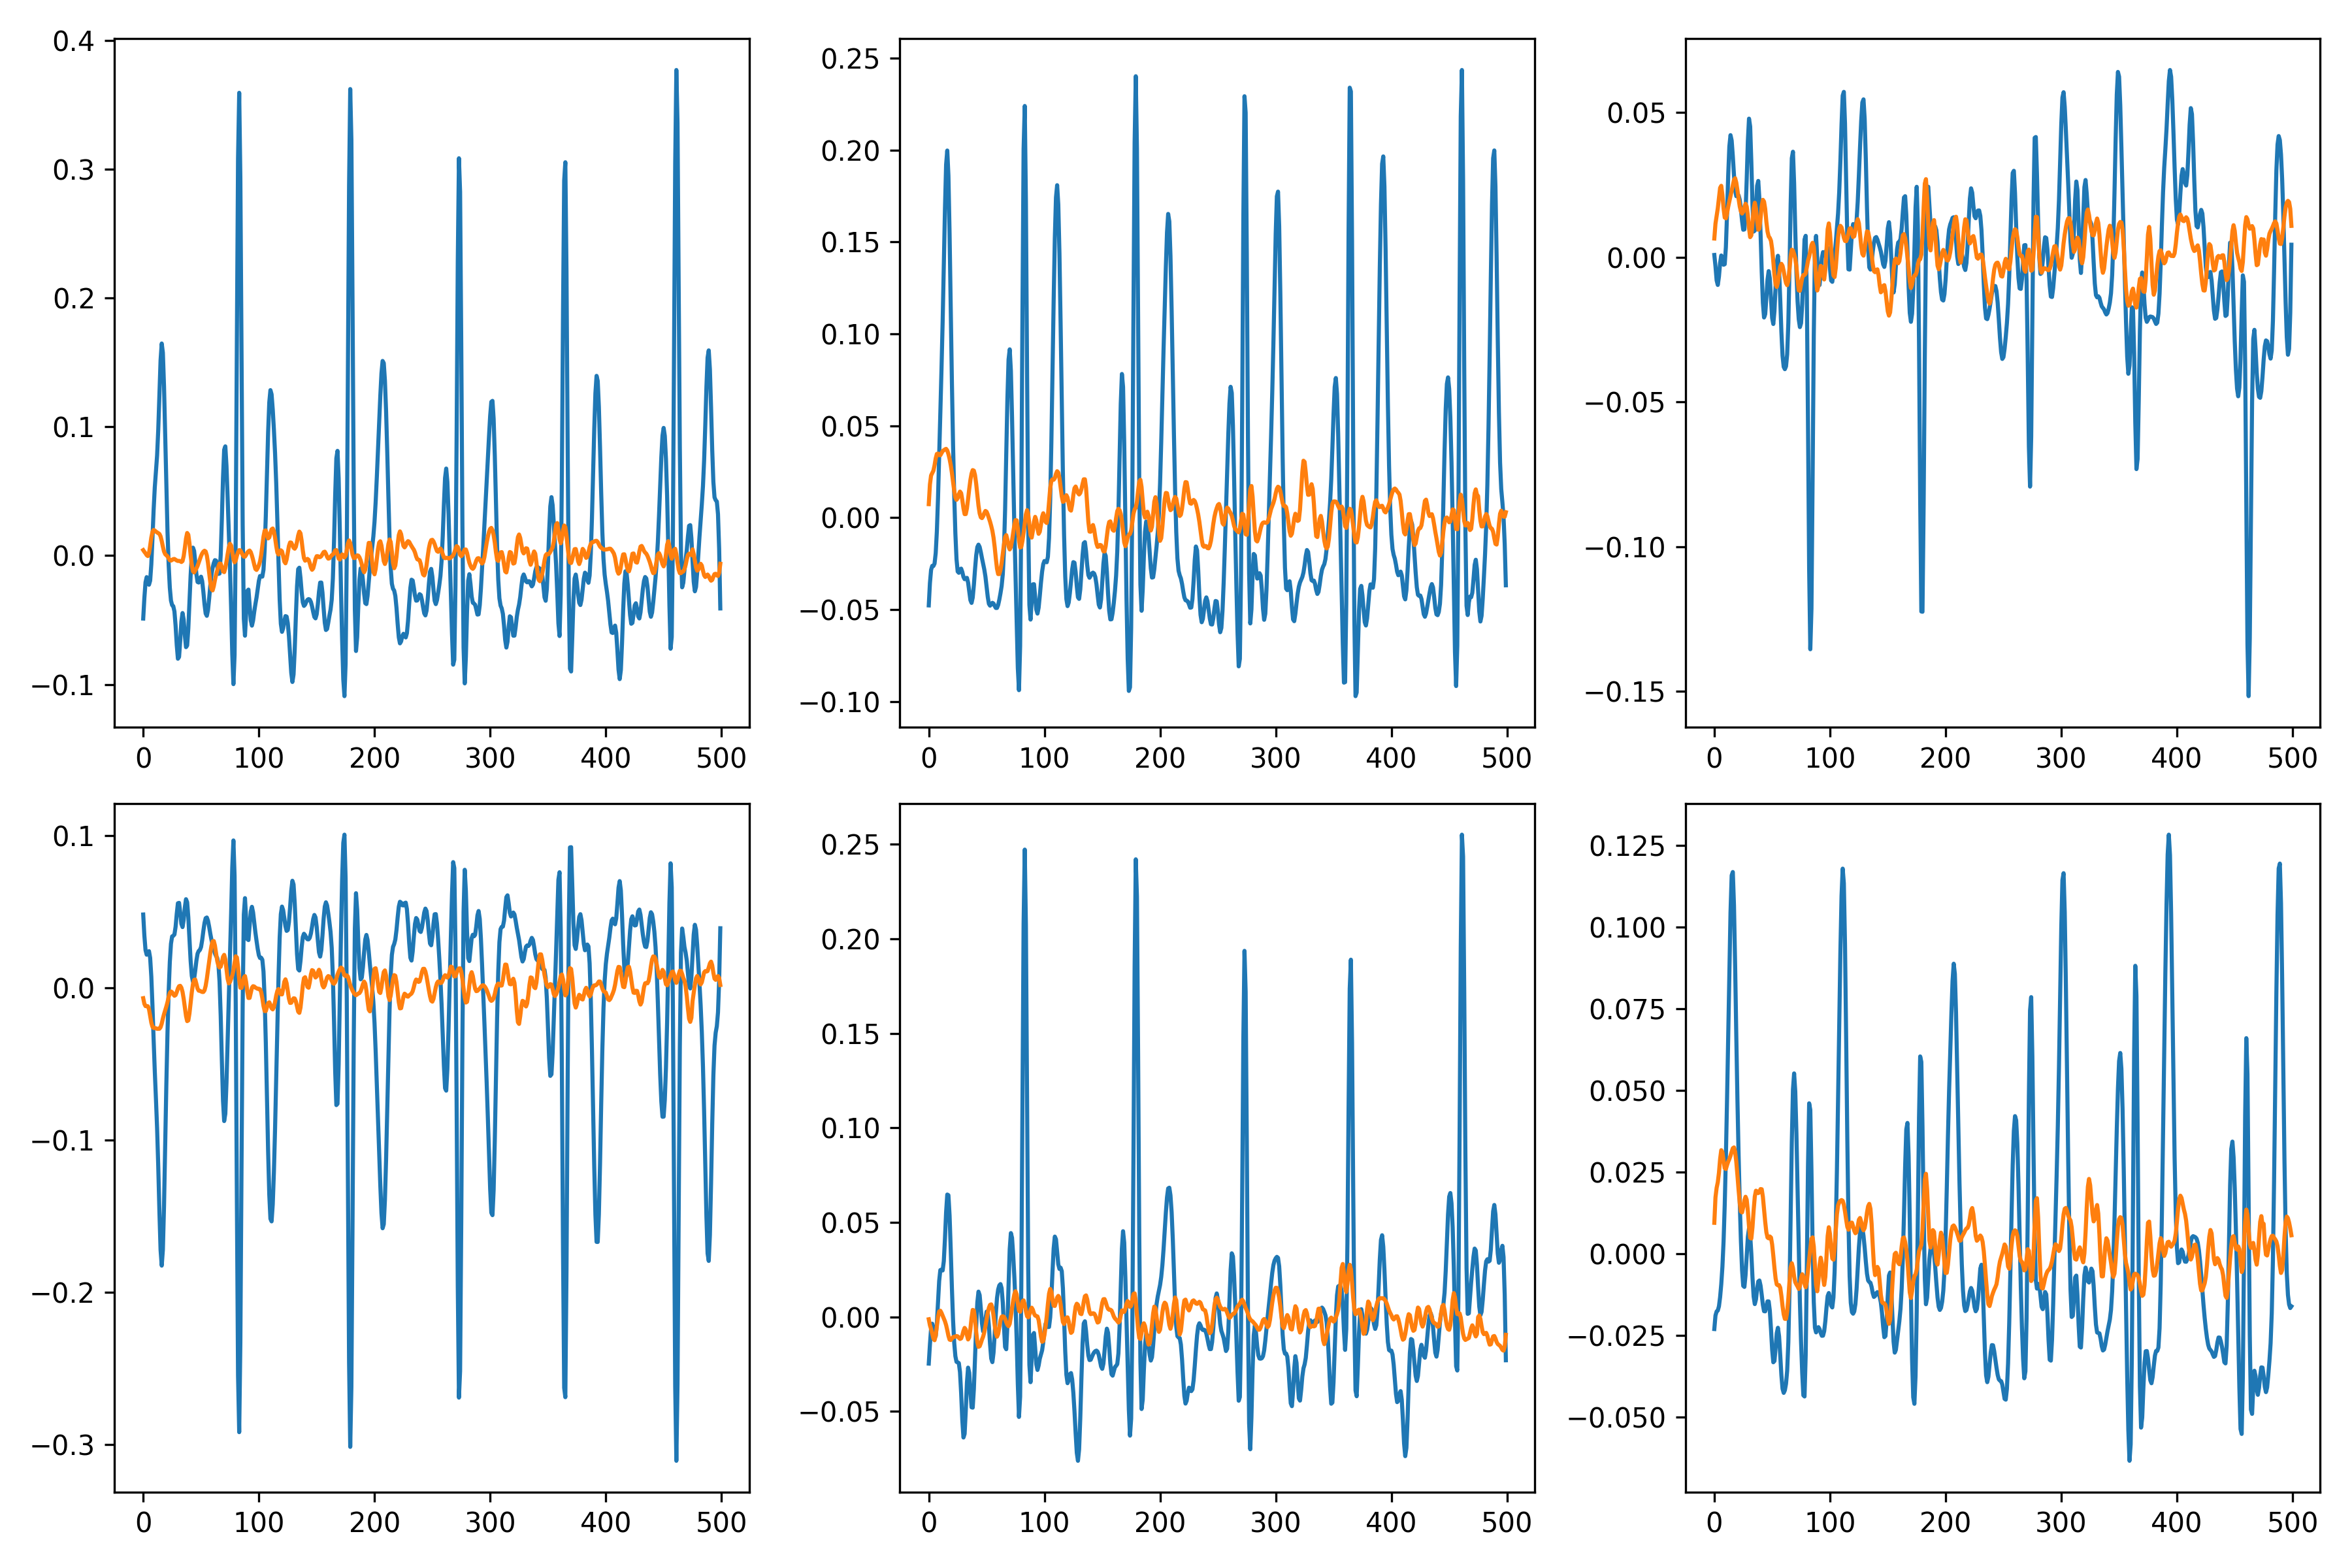
\includegraphics[width=0.85\textwidth]{immagini/terza_cnn_secondo_plot_0.png}
    \captionsetup{justification=centering}
    \caption{Risultati ottenuti dai test effettuati con la terza CNN implementata e testata.}
    \label{fig:terza_cnn_secondo_plot_0}
\end{figure}
\begin{figure}[H]
    \centering
    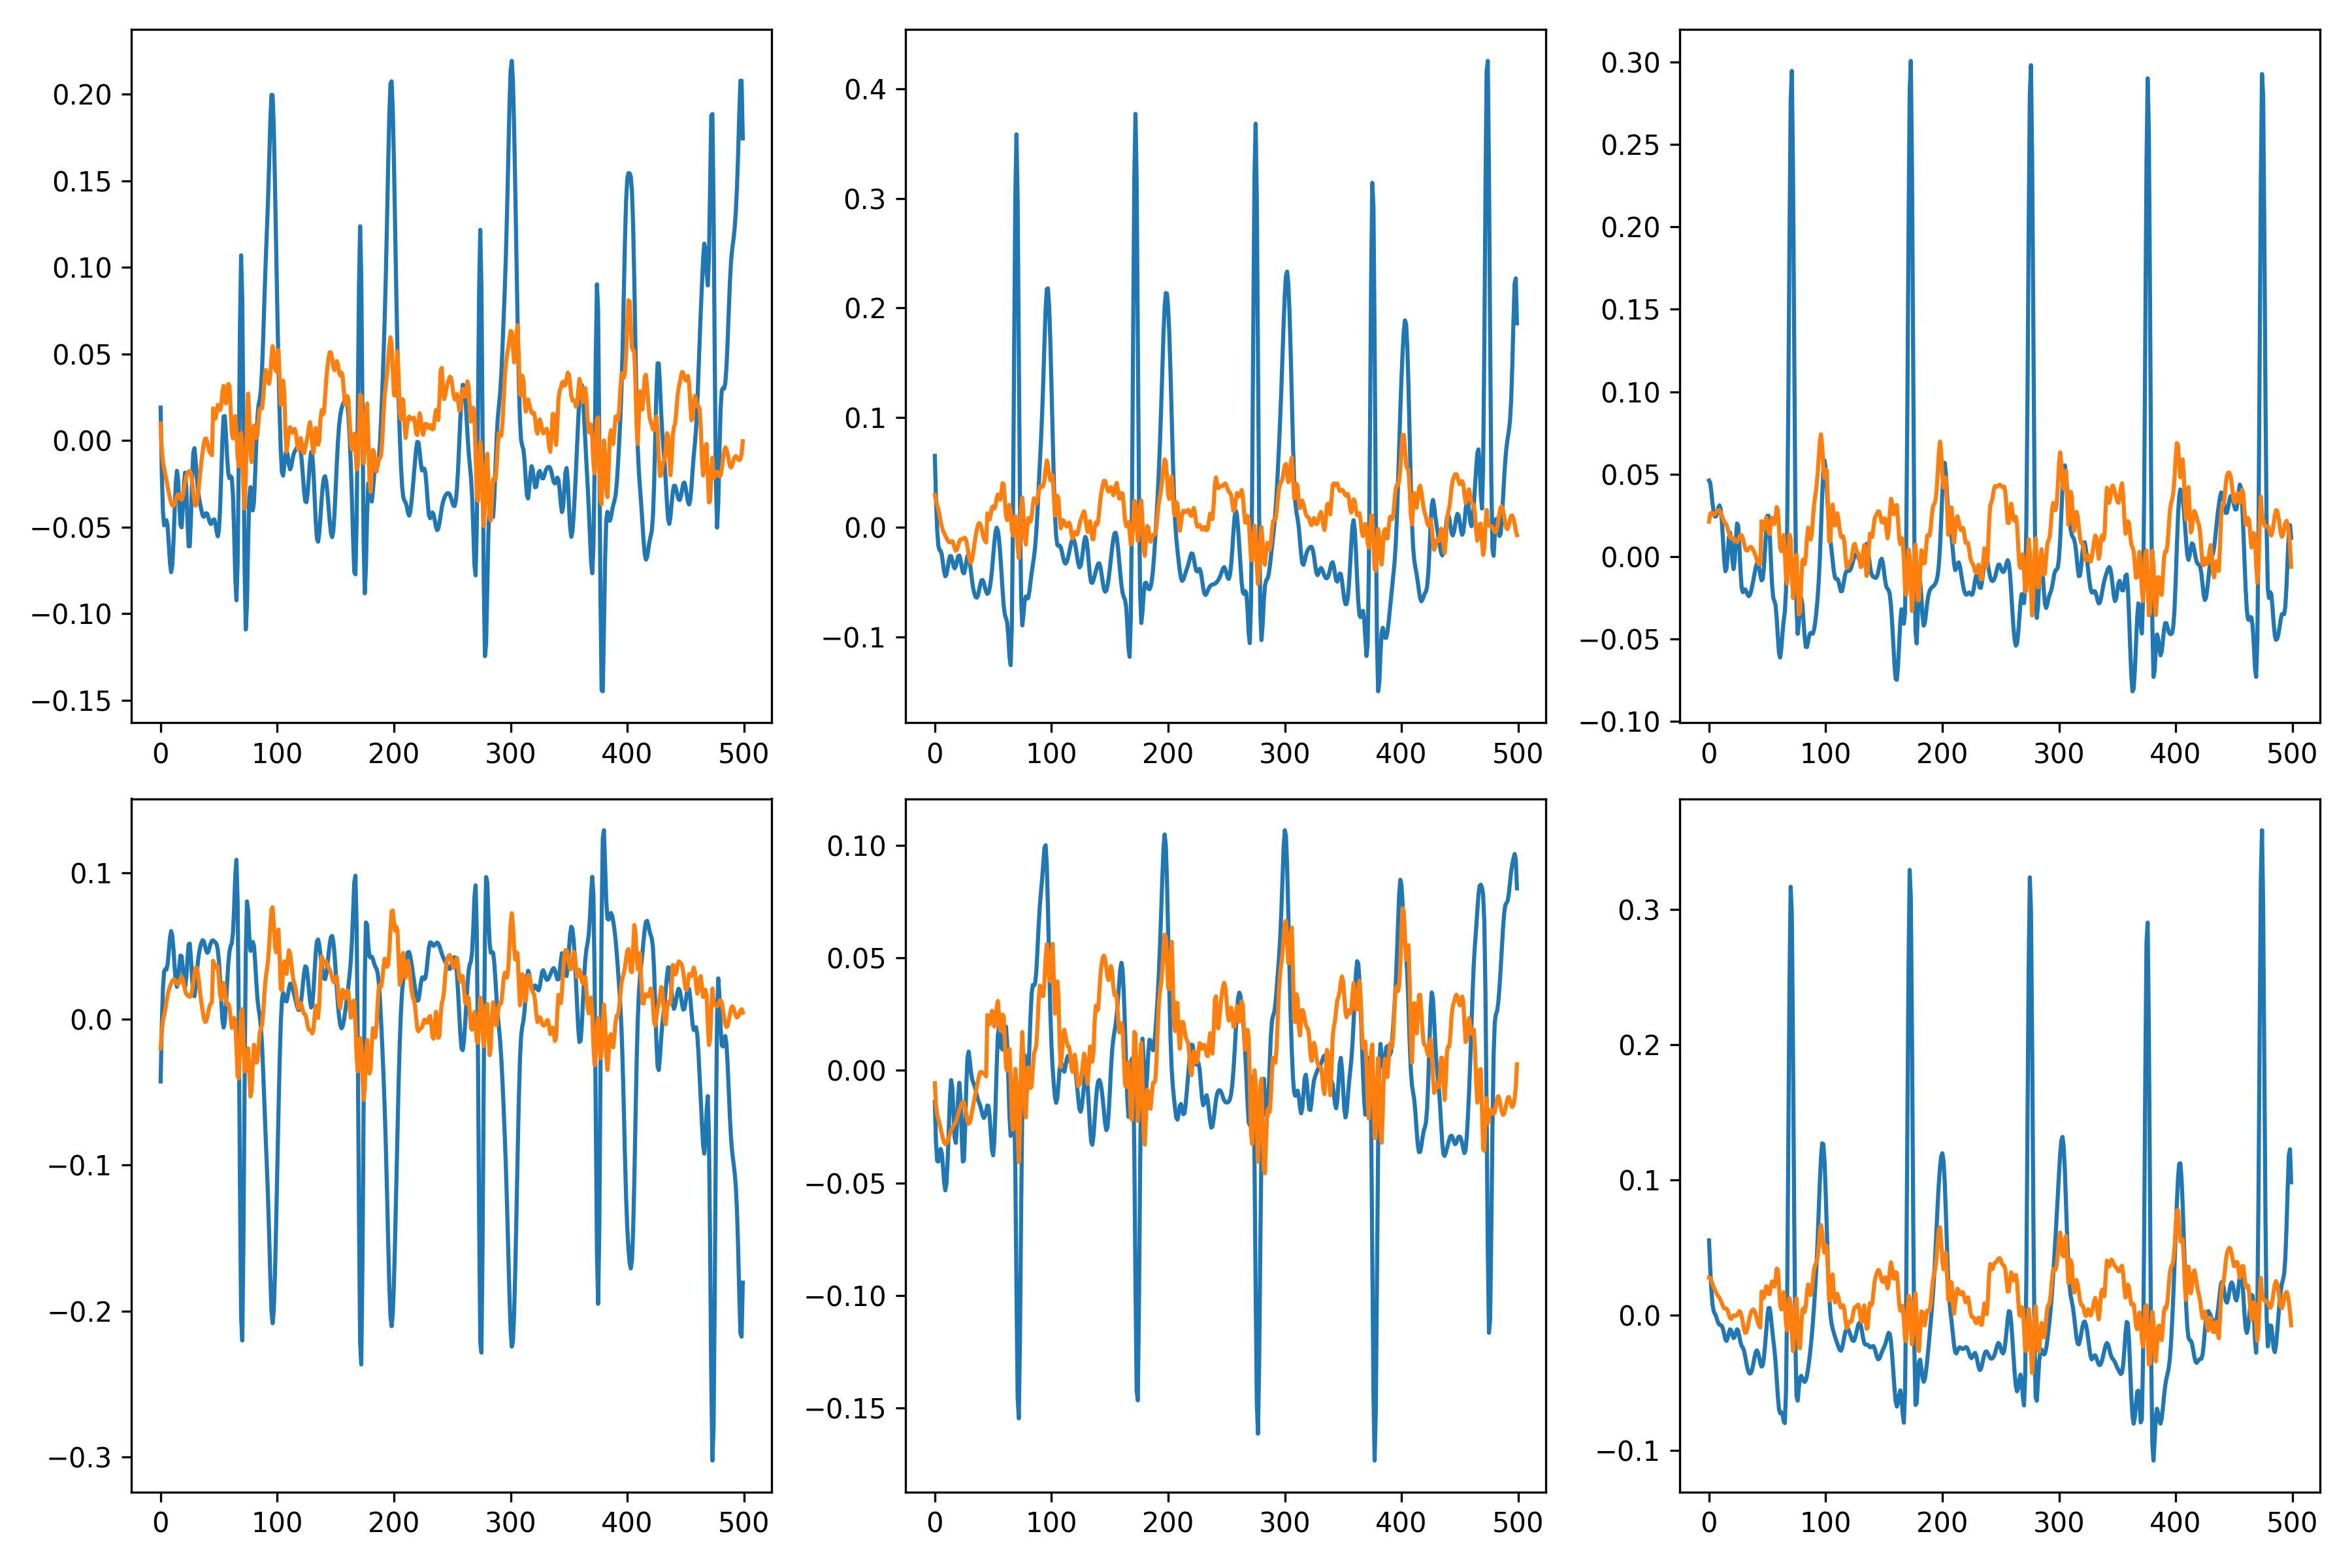
\includegraphics[width=0.85\textwidth]{immagini/terza_cnn_secondo_plot_1.png}
    \captionsetup{justification=centering}
    \caption{Risultati ottenuti dai test effettuati con la terza CNN implementata e testata.}
    \label{fig:terza_cnn_secondo_plot_1}
\end{figure}

\section{Risultati prodotti dalle reti post-clustering}
\label{sec:clustering_risultati}

Nonostante in teoria l'applicazione dell'algoritmo di clustering avrebbe dovuto migliorare in maniera considerevole i risultati prodotti dai test delle varie reti, come si può osservare dalle figure \ref{fig:prima_cnn_risultati_secondo_plot_0},  \ref{fig:prima_cnn_risultati_secondo_plot_1}, \ref{fig:seconda_cnn_risultati_secondo_plot_0} e \ref{fig:seconda_cnn_risultati_secondo_plot_1} riportate di seguito, ancora una volta questi non si sono rivelati completamente soddisfacenti, nonostante rispetto ai risultati precedenti siano comunque migliori e per cui si può dunque denotare un progresso non indifferente dato dalla semplificazione del dataset:

\begin{figure}[H]
    \centering
    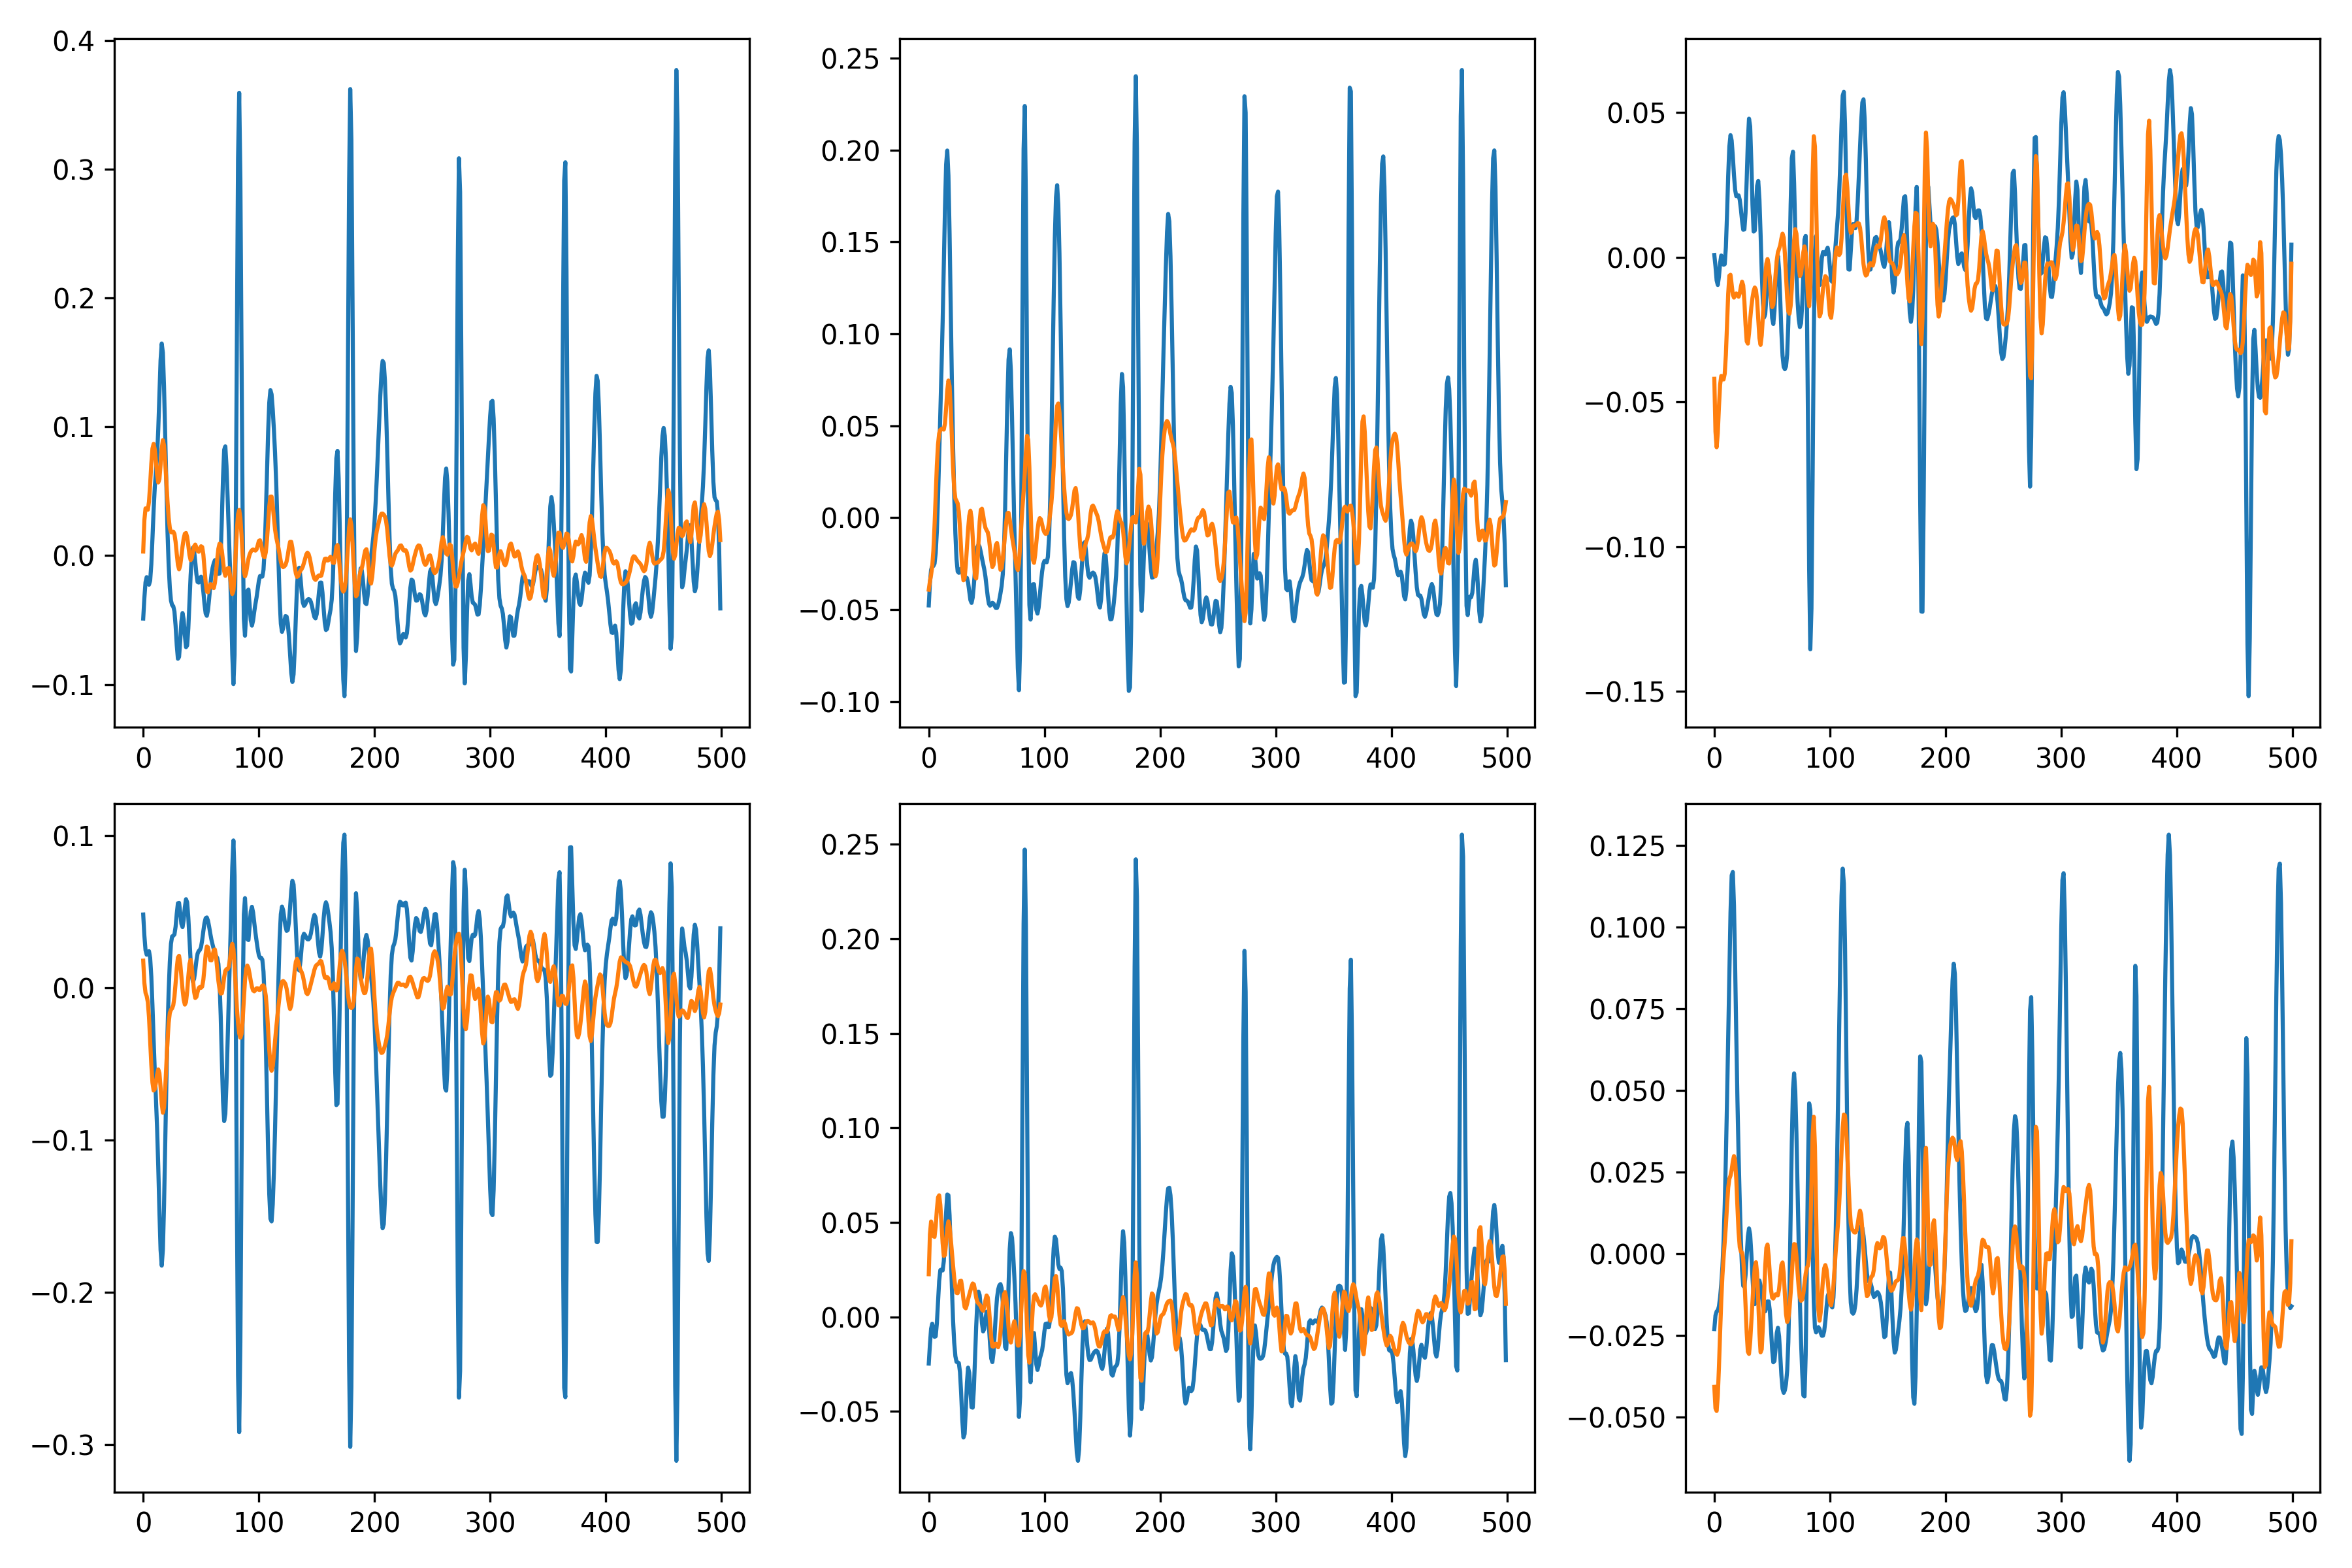
\includegraphics[width=0.85\textwidth]{immagini/prima_cnn_risultati_secondo_plot_0.png}
    \captionsetup{justification=centering}
    \caption{Risultati ottenuti dai test effettuati in seguito alla semplificazione del dataset.}
    \label{fig:prima_cnn_risultati_secondo_plot_0}
\end{figure}
\begin{figure}[H]
    \centering
    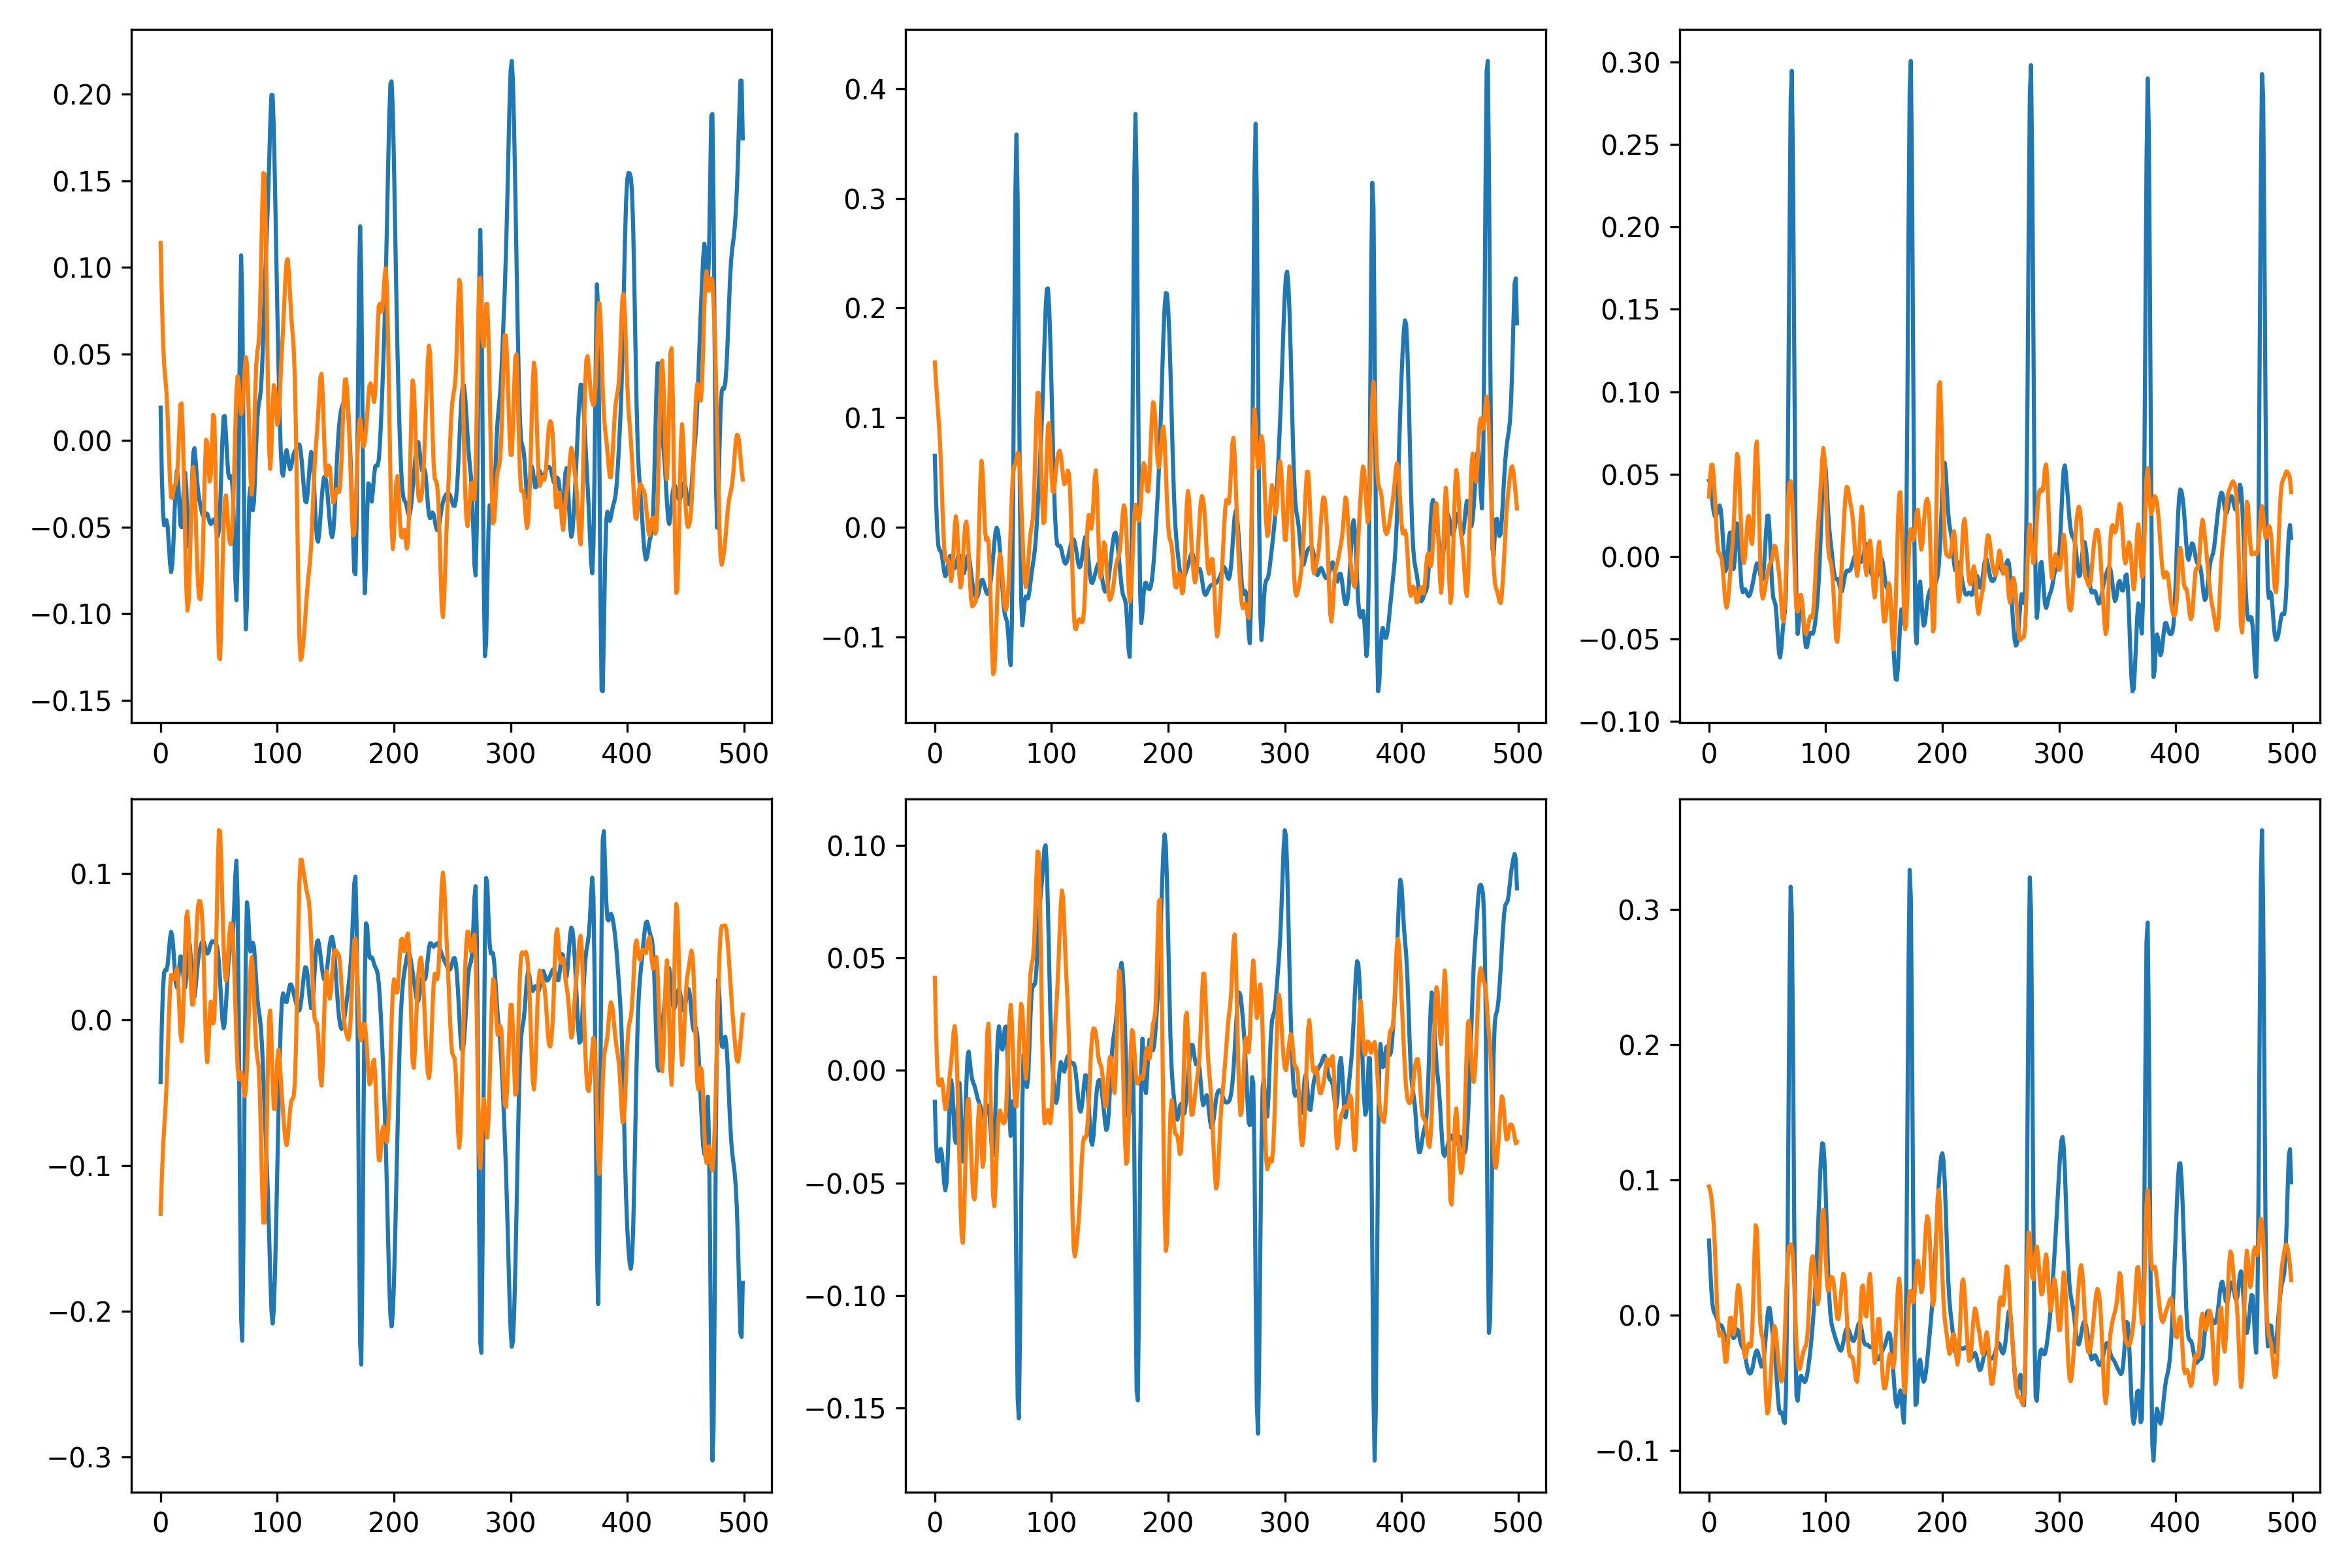
\includegraphics[width=0.85\textwidth]{immagini/prima_cnn_risultati_secondo_plot_1.png}
    \captionsetup{justification=centering}
    \caption{Risultati ottenuti dai test effettuati in seguito alla semplificazione del dataset.}
    \label{fig:prima_cnn_risultati_secondo_plot_1}
\end{figure}
\begin{figure}[H]
    \centering
    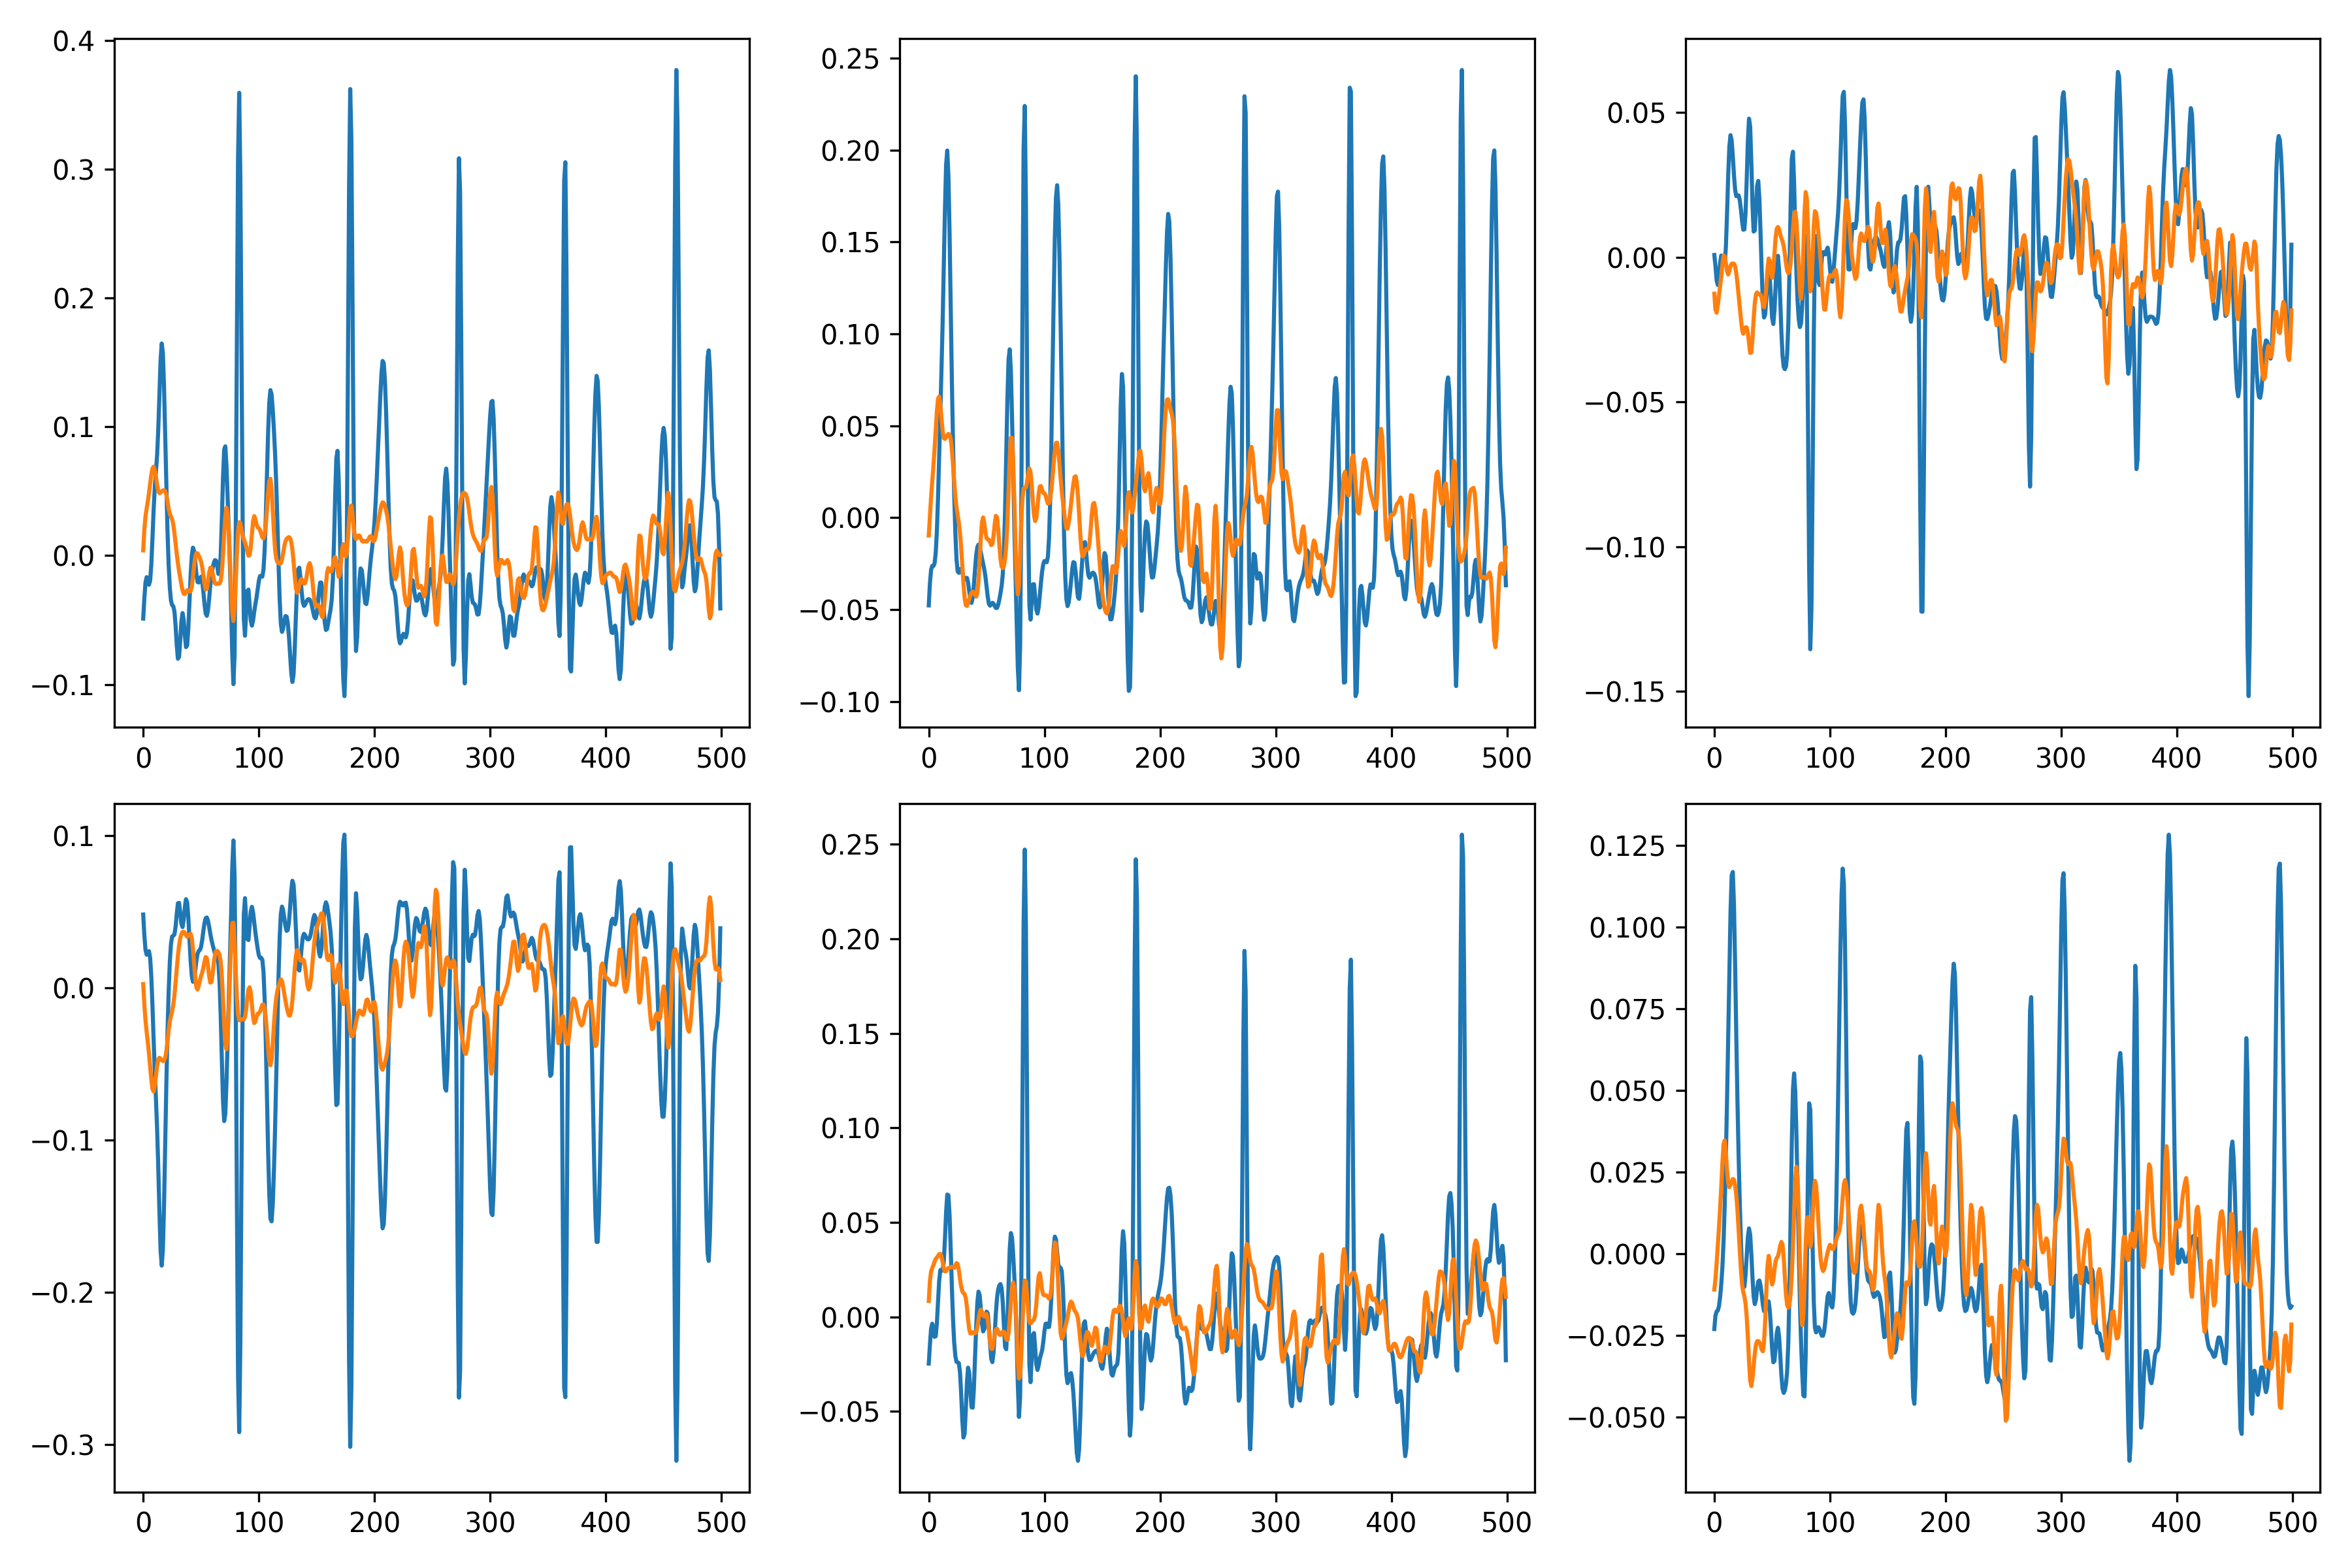
\includegraphics[width=0.85\textwidth]{immagini/seconda_cnn_risultati_secondo_plot_0.png}
    \captionsetup{justification=centering}
    \caption{Risultati ottenuti dai test effettuati in seguito alla semplificazione del dataset.}
    \label{fig:seconda_cnn_risultati_secondo_plot_0}
\end{figure}
\begin{figure}[H]
    \centering
    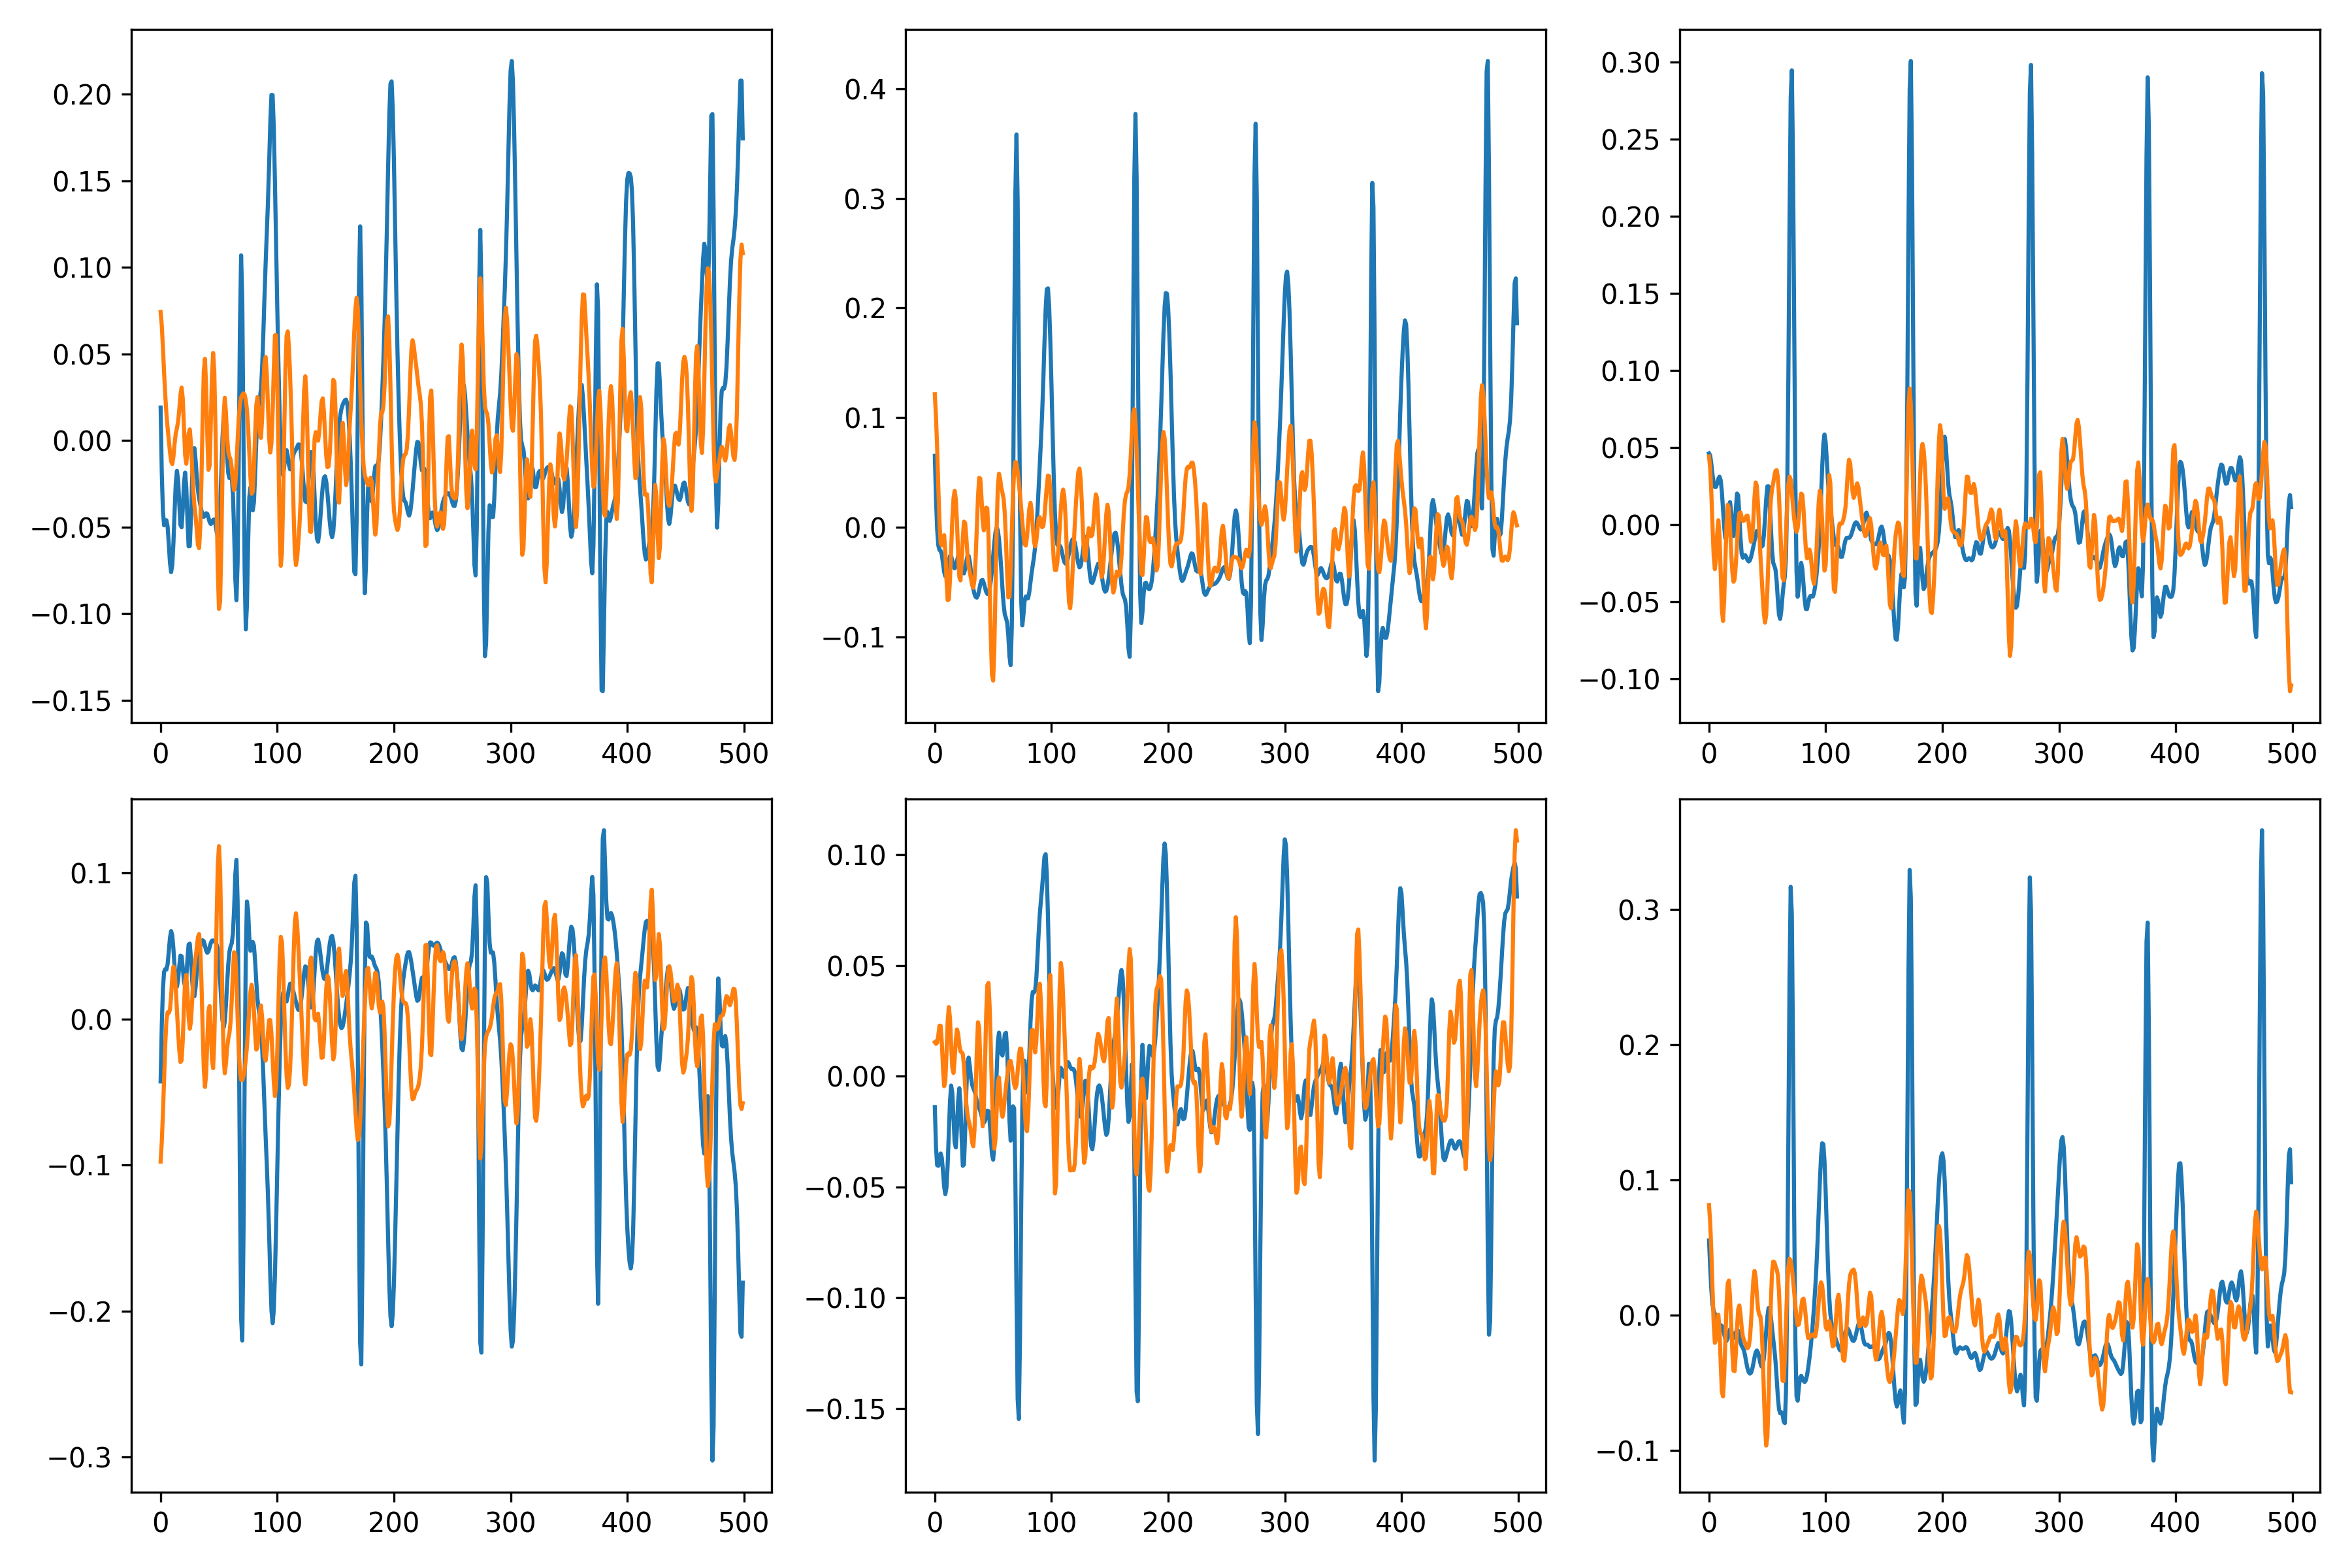
\includegraphics[width=0.85\textwidth]{immagini/seconda_cnn_risultati_secondo_plot_1.png}
    \captionsetup{justification=centering}
    \caption{Risultati ottenuti dai test effettuati in seguito alla semplificazione del dataset.}
    \label{fig:seconda_cnn_risultati_secondo_plot_1}
\end{figure}

\section{Discussione}
\label{sec:discussione}

Come precedentemente detto più volte, purtroppo i risultati ottenuti durante i mesi di test della ricerca non sono stati soddisfacenti e non hanno incontrato le aspettative e le previsioni inizialmente auspicate. Tuttavia, è importante sottolineare che, nell'utilizzo del \textit{deep learning}, non è mai scontato raggiungere immediatamente risultati ottimali. Questa situazione non è unica nel campo del \textit{deep learning}: spesso è necessario eseguire numerosi test e sperimentazioni per trovare la configurazione ottimale che porti ai risultati desiderati.

Nonostante ciò, è stato invece ottenuto un risultato di entropia coerente e significativo rispetto alle aspettative. L'entropia misurata riflette in modo efficace il grado dei dati ed offre un'adeguata misura quantitativa della complessità del sistema studiato. Questo risultato conferma la validità dell'approccio metodologico adottato e fornisce ulteriori prove della robustezza delle analisi effettuate.

Infine, per quanto concerne le tre CNN riportate nella sezione ``Rete neurale convoluzionale'' (Cap. \ref{chap:materiali} Sez. \ref{sec:network}), il fatto di non aver ottenuto da nessuna di esse, comprese inoltre le CNN non presenti e non riportate, dei risultati accettabili, non rappresenta comunque un problema: questa è una caratteristica intrinseca del \textit{deep learning}, in cui il processo di addestramento delle reti neurali può essere influenzato da numerosi fattori, tra cui la complessità del problema, la dimensione e la qualità del dataset, la scelta dell'architettura della rete neurale e dei parametri di addestramento. Durante il periodo di ricerca, sono state implementate e testate numerose e diverse architetture di reti neurali e sono state esplorate varie configurazioni di iperparametri al fine di migliorarne le prestazioni. Tuttavia, nonostante gli sforzi e l'approccio sistematico seguito, i risultati ottenuti non hanno soddisfatto completamente le aspettative. Ciò che è risultato particolarmente singolare è la distanza, in termini di complessità, tra tutte le CNN, ed in particolare tra le tre sopra citate, che ha portato a domandarsi come mai nessuna tra queste, ``semplice'', ``intermedia'', e più ``articolata'', abbia portato dei veri e netti miglioramenti in termini di risultati.

Questo è stato ancor più enfatizzato a seguito dell'applicazione dell'algoritmo di clustering, poiché nonostante la scelta di operare solo con ECG tra loro simili tramite la riduzione della complessità, tutte le reti testate non hanno comunque prodotto i risultati auspicati.

Per concludere, il processo di ricerca e sperimentazione è intrinsecamente caratterizzato da prove ed errori, e il successo non è garantito in anticipo. In sintesi, è comunque fondamentale considerare i risultati come parte integrante del processo di ricerca stesso: difatti questa esperienza ha fornito preziose intuizioni, ha contribuito a migliorare la comprensione del problema in esame ed ha aperto la strada ad ulteriori ricerche e sviluppi futuri per quanto concerne questo problema.

\chapter{Conclusioni}
\label{chap:conclusioni}

Elettrocardiografia e \textit{deep learning} sono, al giorno d'oggi, un binomio sempre più attuale e sempre più soggetto ad essere utilizzato nella pratica per migliorare la precisione e l'efficienza nella diagnosi e nella classificazione delle condizioni cardiache.

L'altra faccia della medaglia riguarda invece la mancanza di set di dati adeguati per l'addestramento delle reti, nonché la mancanza di precise ed adeguate procedure di valutazione in grado di garantire la similarità di diversi algoritmi. Infatti, uno dei principali aspetti nell'applicazione del \textit{deep learning} all'analisi degli ECG è la disponibilità di dataset di addestramento ampi e di alta qualità: la raccolta e l'annotazione di questi dataset rappresentano ancora una sfida significativa che richiede un notevole sforzo umano e una collaborazione tra i medici ed i ricercatori.

Nonostante queste sfide, i risultati ottenuti finora sono estremamente promettenti: la combinazione di competenze mediche e conoscenze di \textit{deep learning} sta aprendo nuove prospettive, e l'utilizzo del \textit{deep learning} nell'analisi degli ECG rappresenta un campo di ricerca in rapida evoluzione che sicuramente avrà un ruolo sempre più di maggior rilievo nella pratica clinica cardiologica.

Gli ECG standard sono costituiti da 12 derivazioni usate per registrare i potenziali elettrici degli atri e dei ventricoli del cuore. In questa tipologia di ECG, quattro elettrodi vengono posizionati sugli arti del paziente e sei sulla superficie del torace, e dunque il potenziale elettrico complessivo del cuore viene misurato in dodici differenze tra punti, comunemente chiamate ``derivazioni'', e registrato per un periodo di tempo stabilito a priori, solitamente pari a dieci secondi. Dunque la corretta interpretazione dell'ECG è possibile con un tracciato a 12 derivazioni di ottima qualità ed è consigliabile seguire un approccio sistematico che consenta di procedere secondo un ordine prestabilito.

L'elettrocardiografia permette la rilevazione di moltissime condizioni cardiache, ma viene anche usata per monitorare in maniera continuativa i pazienti cardiaci, registrando l'attività elettrica del cuore e consentendo così una valutazione dettagliata.

In relazione agli ECG a 12 derivazioni sono di fondamentale importanza i segnali di Frank, che rappresentano una metodologia di acquisizione elettrocardiografica che fornisce informazioni dettagliate sulla distribuzione spaziale dell'attività elettrica del cuore. A differenza degli ECG standard a 12 derivazioni, i segnali di Frank permettono di acquisire una mappa più completa dell'attività elettrica cardiaca, consentendo una diversa valutazione della morfologia degli impulsi elettrici, nonché delle anomalie e dei disturbi cardiaci.

L'obiettivo della ricerca è stato quello di ricostruire, a partire da un ECG, il segnale che idealmente lo susseguirebbe nel tempo. Poiché nelle cliniche si utilizzano ancora moltissimo gli ECG cartacei che hanno una durata pari a dieci secondi, dei quali i primi cinque mostrano i primi 6 \textit{lead} dell'ECG mentre i restanti cinque mostrano i restanti 6 \textit{lead} dell'ECG, l'obiettivo è stato quello di ricostruire i \textit{lead} che non vengono osservati, e cioè i primi 6 nei secondi cinque secondi, ed i secondi 6 nei primi cinque secondi.

Il dataset utilizzato durante la ricerca è stato individuato in \textit{PTB-XL}, un dataset esteso di ECG sviluppato in Germania e contenente registrazioni di segnali ad alta risoluzione, sia a 12 derivazioni che a 15 derivazioni. Il dataset contiene sia ECG di pazienti sani che ECG di pazienti affetti da anomalie cardiache, per un totale di 21799 ECG a 12 derivazioni provenienti da 18869 pazienti, con una durata di 10 secondi ciascuno. Inoltre, il dataset è integrato da metadati dettagliati sulla demografia, sulle caratteristiche di infarto, sulla probabilità delle dichiarazioni diagnostiche e sulle proprietà segnalate. Durante il processo di pubblicazione nel 2019, il dataset è stato ottimizzato con particolare attenzione all'usabilità ed all'accessibilità per la comunità di \textit{deep learning}, in modo tale che i dati che possano essere facilmente elaborati da software standard.

Tuttavia, poiché il dataset include anche ECG di pazienti affetti da anomalie cardiache, è stato dapprima necessario effettuare un filtraggio dei segnali per operare esclusivamente con gli ECG di pazienti sani.

Durante la ricerca sono emersi molti problemi inizialmente inaspettati, ed è stato dunque necessario applicarsi per trovare il modo di ottenere i risultati sperati: uno di questi è stato applicare il calcolo dell'entropia, che fornisce una base per prese di decisione, ottimizzazione e comprensione del problema da risolvere.

Per effettuare poi la vera e propria ricostruzione degli ECG sono state introdotte diverse e numerose reti di tipologia \textit{convolutional neural network}, implementate, testate ed adattate più volte in cerca di buoni risultati. In particolare, sono state implementate reti riassumibili e raggruppabili in tre distinte tipologie: reti semplici formate solamente da un insieme di layer convoluzionali, reti formate da questo stesso insieme di layer unito ad una componente esterna introdotta per affrontare il problema del degrado delle performance, ed infine reti molto più articolate formate da più componenti intrecciate ed operanti all'unisono. Purtroppo nessuna di queste tipologie ha portato i risultati auspicati, verificati tramite l'osservazione dei risultati e tramite la funzione \texttt{MSE}, abbreviazione di \textit{Mean Squared Error}. Tuttavia, è stato molto utile implementare e testare reti così diverse in termini di complessità, che è dunque sempre stata incrementale, per osservare alla fine come i risultati si sono evoluti e sono cambiati nel tempo nel corso dei test.

Tuttavia, dopo aver verificato ancora una volta gli insoddisfacenti risultati da parte di tutte le CNN implementate, l'idea è stata quella di semplificare il più possibile i dati sui quali effettuare l'addestramento, adottando dunque l'algoritmo di clustering \textit{K-means}, per raggruppare gli ECG con caratteristiche simili in diversi \textit{cluster}. In tal modo, idealmente le CNN dovrebbero produrre risultati migliori, vista la similarità tra i segnali, mantenendone comunque un cospicuo numero totale, fondamentale per il corretto addestramento delle reti.

Attraverso un'approfondita analisi svolta durante l'intero periodo di ricerca, sono stati ottenuti risultati significativi che contribuiscono a comprendere quanto sia complicato e per nulla scontato ottenere risultati soddisfacenti nel solo tempo dedicato al lavoro di tesi, potendo svolgere un numero finito di test che non sempre risultano fortuiti in termini di risultati. Tuttavia, è importante notare come questa ricerca presenti alcune limitazioni, come quelle di natura temporale e quelle legate al dataset utilizzato, legate alla bontà dei dati ed alla dimensione estesa, che ha richiesto diverso tempo per l'esecuzione e per i test. Nonostante ciò, questo lavoro rappresenta un passo in avanti per la ricostruzione dei segnali elettrocardiografici ed offre spunti interessanti per future indagini e ricerche. Si può quindi dire con assoluta certezza che questa ricerca ha espresso in modo molto marcato l'importanza dell'utilizzo dell'IA e del \textit{deep learning}, e fornisce una base solida per ulteriori esplorazioni in un campo che è, giorno dopo giorno, in continua e rapida evoluzione.

\afterpage{\blankpage}

\bibliographystyle{unsrt}
\bibliography{bibliografia}
\addcontentsline{toc}{chapter}{Bibliografia}

\afterpage{\blankpage}

\end{document}
